\documentclass[11pt]{article}

% Paquete para configurar márgenes y espaciado
\usepackage[a4paper, margin=2.5cm]{geometry}

% Paquete para el manejo de idiomas y codificación de fuentes
\usepackage[spanish]{babel}
\usepackage[utf8]{inputenc}
\usepackage[T1]{fontenc}

% Configuración de fuentes
\usepackage{mathptmx} % Times New Roman
\renewcommand{\rmdefault}{ptm}

% Configuración de títulos
\usepackage{titlesec}
\titleformat*{\section}{\fontsize{16}{18}\bfseries}
\titleformat*{\subsection}{\fontsize{14}{16}\bfseries}
\titleformat*{\subsubsection}{\fontsize{14}{16}\bfseries}

% Configuracion de bibliografia
\usepackage{fvextra}
\usepackage[autostyle,spanish=spanish]{csquotes}

\usepackage[backend=biber,refsegment=section,defernumbers=true]{biblatex}
\addbibresource{resources/bibliography.bib} 
\addbibresource{resources/repos.bib} 

% Configuración de interlineado
\usepackage{setspace}
\onehalfspacing

% Configuración de encabezado y pie de página
\usepackage{fancyhdr}
\pagestyle{fancy}
\fancyhf{}
\chead{Análisis de lenguajes para sistemas concurrentes}
\rfoot{\thepage}
\lfoot{Civini, Foppiano, Mastricchio, Zulaica}

% Configuracion para que las imagenes no floten a otras secciones / sub-secciones

\usepackage{placeins}

\let\Oldsection\section
\renewcommand{\section}{\FloatBarrier\Oldsection}

\let\Oldsubsection\subsection
\renewcommand{\subsection}{\FloatBarrier\Oldsubsection}

\let\Oldsubsubsection\subsubsection
\renewcommand{\subsubsection}{\FloatBarrier\Oldsubsubsection}

% Configuración de espacio antes y después de los párrafos
\setlength{\parskip}{0pt}
\setlength{\parindent}{2em}
\setlength{\headheight}{13.6pt}

\usepackage{graphicx}


\usepackage{amsmath}

\PassOptionsToPackage{hyphens}{url}
\usepackage[colorlinks = true,
            linkcolor = blue,
            urlcolor  = blue,
            citecolor = blue,
            anchorcolor = blue]{hyperref}
\usepackage[table,xcdraw,dvipsnames]{xcolor}
\usepackage{svg}


\usepackage[newfloat]{minted}
\usepackage{cleveref}

\usemintedstyle{default}
\definecolor{bg}{RGB}{248,248,248}
% \definecolor{bg}{HTML}{282828}
\usepackage{listings}
\lstset{
  basicstyle=\ttfamily,
  columns=fullflexible,
  breaklines=true,
  postbreak=\mbox{{$\hookrightarrow$}\space},
}

\usepackage{algorithm}
\usepackage{algpseudocode}
\renewcommand*\Call[2]{\textproc{#1}(#2)}

\usepackage{caption}

\newenvironment{code}{\captionsetup{type=listing}}{}
\SetupFloatingEnvironment{listing}{name=Código}

\usepackage{float}

\newcommand{\badMetric}[1]{{\color{BrickRed}#1}}

\newcommand{\goodMetric}[1]{{\textbf{#1}}}

\usepackage{multirow}

\providecommand{\row}[1]{\parbox{150pt}{\setlength{\baselineskip}{0.2\baselineskip}\strut#1\strut}}

\usepackage{multicol}

\renewcommand{\arraystretch}{1.4}

\usepackage{plantuml}
\usepackage{amsfonts} 
\usepackage{subcaption}

% Set figure/code/table numbering per section
\counterwithin{figure}{section}
\counterwithin{table}{section}
\counterwithin{listing}{section}

\newcommand{\ipcap}[2]{\caption{Métricas de #1 para el caso de uso de Procesamiento de Imágenes, corridas en #2}}
\newcommand{\gscap}[2]{\caption{Métricas de #1 para el caso de uso de Grid Search, corridas en #2}}

\newcommand{\mail}[1]{\href{mailto:#1}{\nolinkurl{#1}}}

\newcommand{\english}[1]{\textit{#1}}
\newcommand{\technical}[1]{\textit{#1}}

\usepackage{numprint}
\npthousandsep{.}




\setpythontexlistingenv{pythontexlisting}
\begin{document}

% Carátula temporal
\begin{titlepage}

\begin{center}
	\begin{minipage}{2.5cm}
	\begin{center}
		
\includegraphics[width=\textwidth]{cover/uba_logo.png}
		
	\end{center}
\end{minipage}\hfill
\begin{minipage}{8cm}
	
\end{minipage}\hfill
\begin{minipage}{4cm}
	\begin{center}
		
\includegraphics[width=\textwidth]{cover/fiuba_logo.png}
	\end{center}
\end{minipage}

\vspace{1cm}

\begin{center}
	{\Huge \textbf{Universidad de Buenos Aires}}\\[0.5cm]
    {\huge Facultad de Ingeniería}
\end{center}
 


\textsc{\Large }\\[1.5cm]
{\huge Trabajo Profesional de Ingeniería en Informática}\\[0.5cm]

\vspace{1cm}

% Title
\rule{\linewidth}{0.3mm} \\[0.4cm]
{ \Huge \bfseries Análisis de lenguajes para sistemas concurrentes \\[0.4cm] }
\rule{\linewidth}{0.3mm} \\[2cm]


\begin{table}[H]
\centering
\begin{tabular}{|l|c|l|}
\hline
\rowcolor[HTML]{EFEFEF} 
Apellido, Nombre & Padrón & Correo Electrónico \\ \hline
Civini, Armando Tomás & 104350 & \mail{acivini@fi.uba.ar} \\ \hline
Foppiano, Elián Daniel & 105836 & \mail{efoppiano@fi.uba.ar} \\ \hline
Mastricchio, Facundo Rodrigo & 100874 & \mail{fmastricchio@fi.uba.ar} \\ \hline
Zulaica Rivera, Nicolás Ezequiel & 105774 & \mail{nzulaica@fi.uba.ar} \\ \hline
\end{tabular}
\end{table}

\vfill

% Bottom of the page
{\textbf{\large Junio 2024}}

\end{center}
\end{titlepage}

\tableofcontents
\newpage

\section{Resumen}


Este trabajo tiene como objetivo evaluar distintos lenguajes de programación y sus entornos, en aplicaciones de sistemas concurrentes. Para lograrlo, se compararon estos lenguajes en cuatro dominios de aplicación: sistemas distribuidos, criptografía, redes neuronales y protocolos de comunicación, con los cuales se buscó resaltar distintos aspectos y desafíos de la concurrencia.

Los resultados de la evaluación permitieron analizar aspectos cuantificables, como el rendimiento de los lenguajes, así como aspectos cualitativos, como la facilidad de uso y el tiempo de desarrollo. Esto nos permitió concluir cuáles herramientas son más adecuadas según el caso de uso y las necesidades específicas de cada aplicación.

\subsection{Palabras clave}

Concurrencia, \english{benchmarks}, lenguajes de programación, entornos de desarrollo, sistemas distribuidos, criptografía, redes neuronales, servidor http, comparación, optimización.

\section{Abstract}

This work aims to evaluate various programming languages and their environments, in applications involving concurrent systems. To achieve it, these languages were compared across four application domains: distributed systems, cryptography, neural networks and communication protocols. The goal was to highlight different aspects and challenges of concurrency within each domain.

The evaluation results enabled the analysis of quantifiable aspects such as language performance, as well as qualitative aspects like ease of use and development time. This allowed us to conclude which tools are most suitable depending on the use case and specific application needs.

\subsection{Keywords}

Concurrency, benchmarks, programming languages, environments, distributed systems, criptography, neural networks, http server, comparisons, optimization.

\newpage

\section{Introducción}

En los últimos años, han surgido nuevos lenguajes de programación y ecosistemas que ofrecen diferentes niveles de abstracción, mecanismos, herramientas y posibilidades para modelar problemas de manera más eficiente. Estos lenguajes y ecosistemas, a menudo no explorados, están empezando a cobrar reconocimiento.

Se presenta un conjunto de dominios de aplicación para el análisis: sistemas distribuidos (particularmente para el procesamiento de datos), algoritmos criptográficos, redes neuronales (dentro del contexto de la ciencia de datos) y protocolos de comunicación (enfocándonos en servidores).

Para cada una de estas áreas, se busca proporcionar una base de métricas y análisis que sea útil para la toma de decisiones a la hora de elegir el ecosistema más adecuado.

Este trabajo propone explorar tanto los ecosistemas más utilizados como aquellos que están ganando popularidad o son aún poco conocidos, aplicándolos a diversos casos de uso con un énfasis especial en sus características concurrentes. La evaluación se realizará desde un punto de vista objetivo, utilizando métricas obtenidas mediante \english{benchmarking}, así como desde un punto de vista subjetivo, comparando aspectos como la facilidad de aprendizaje y uso.

\newpage

\section{Contexto}

\subsection{Estado del arte}

En la actualidad, la concurrencia es un tema central en el desarrollo de software. Gracias a ella, es posible reducir la latencia de aplicaciones que interactúan con el usuario, el disco, la red y dispositivos de IoT, entre otros. Además, mejora la \english{performance} de tareas de procesamiento intensivo en ambientes \english{multi-core} (CPU) y \english{many-core} (GPU).

Sin embargo, desarrollar una aplicación concurrente presenta múltiples desafíos, como la dificultad para realizar \textit{debugging} y \textit{testing}, la pérdida de determinismo y la aparición de nuevos tipos de errores propios de este ambiente.

Estos desafíos han favorecido el surgimiento de muchas tecnologías, incluyendo el desarrollo de lenguajes de programación con la concurrencia como uno de sus objetivos principales \cite{rust:ex:fearless_concurrency} \cite{go:ex:concurrency_patterns}, \textit{frameworks} de \textit{benchmarking}, e incluso nuevos modelos de computación concurrente con sus respectivas implementaciones \cite{state_of_the_art:reactors}. También se han desarrollado versiones concurrentes de diversos algoritmos para favorecer el paralelismo \cite{state_of_the_art:huffman_gpu}.

A día de hoy, muchos trabajos se centran en comparar diferentes algoritmos implementados en el mismo ecosistema \cite{state_of_the_art:crypto_benchmarks} \cite{state_of_the_art:nn_benchmarks}, así como en realizar comparaciones prestaciones entre lenguajes para problemas básicos \cite{state_of_the_art:lang_benchmarks}.

\subsection{Oportunidad de mejora}

Nuestra propuesta es comparar diferentes lenguajes y ecosistemas, en contraste con estudios centrados en ecosistemas particulares.
Desarrollando diversas aplicaciones y casos de uso de la vida real en la industria, agregando complejidades que se pueden ver omitidas en los problemas básicos.
Poniendo un enfoque sobre las herramientas que utilizamos, evaluando tanto el impacto sobre el producto final así como en el proceso de desarrollo.

\subsection{Entornos de despliegue} \label{sec:deploy_envs}

Se obtuvo acceso a dos supercomputadoras de la Universidad de Córdoba (Facultad de Matemática, Astronomía, Física y Computación - FaMAF y del Centro de Cómputo de Alto Desempeño - CCAD), gracias a la colaboración de Rosa Wachenchauzer y Nicolás Wolovick. De aquí en adelante, llamaremos \textbf{FaMAF-1} y \textbf{FaMAF-2} a cada una de ellas:

\begin{itemize}
    \item \textbf{FaMAF-1}: cuenta con procesador AMD EPYC 7643, 128 GB de memoria RAM, disco SSD de 894 GB, GPU NVIDIA TITAN Xp.
    \item \textbf{FaMAF-2}: cuenta con procesador E5-2680v4, 128 GB de memoria RAM, disco SSD de 223 GB, GPU NVIDIA GeForce RTX 3070
\end{itemize}

Además, para el despliegue de todos los sistemas y aplicaciones, se utilizó Docker \cite{com:docker} para virtualizar el entorno mediante contenedores.

\newpage

\section{Introducción de lenguajes}

Esta sección se introducen brevemente los distintos lenguajes estudiados y sus características en cuanto a la concurrencia.

\subsection{C++}

Es un lenguaje imperativo multiparadigma, compilado, y de tipado estático. Es estándar en la industria, versátil y poderoso. Su primera versión fue lanzada en el año 1983, lo cual lo hace uno de los más antiguos de los seleccionados. Los aspectos generales de su diseño son el rendimiento, la eficiencia y la flexibilidad de uso.

La biblioteca estándar provee mecanismos de sincronización propios del paradigma de estado mutable compartido: semáforos, \english{condition variables} \footnote{\lstinline{std::condition_variable} es una primitiva de sincronización utilizada para bloquear uno o más subprocesos hasta que otro subproceso modifica una variable compartida (la condición) y lo notifica.}, entre otros. También soporta programación asincrónica mediante la función \lstinline{std::async}.

\subsection{Scala}

Es un lenguaje que combina la programación orientada a objetos con la funcional. Está diseñado para ser expresivo, proveyendo abstracciones de alto nivel que aumentan la productividad y simplifican el código; escalable, adaptándose a entornos concurrentes y distribuidos, priorizando la interoperabilidad; y seguro, incluyendo chequeos estáticos y estructuras \english{thread-safe} \cite{com:scala}.

Se ejecuta sobre la JVM (\technical{Java Virtual Machine}), pudiendo hacer uso de muchos recursos del ecosistema de Java. Implementa \english{Futures} como unidad para tareas concurrentes.

\subsection{Go}

Un lenguaje moderno que toma prestadas ideas de otros. Busca construir sistemas simples, seguros y escalables; siendo fácil de aprender y proveyendo herramientas nativas para la concurrencia \cite{com:go}.

Corre sobre un \english{runtime} que se encarga del manejo de memoria. Provee una abstracción nativa para la concurrencia, \technical{gorutinas}, y canales para su comunicación.

\subsection{Julia}

Es un lenguaje orientado a la ciencia de datos y al cómputo de alto rendimiento. Busca ser dinámico, flexible y eficiente \cite{com:julia}. Fue diseñado para combinar la simplicidad de los lenguajes de alto nivel con la velocidad de los lenguajes de bajo nivel.

Corre sobre un \english{runtime} propio y soporta concurrencia basada en tareas, permitiendo la ejecución paralela de bloques de código. Además, provee herramientas nativas para cómputo distribuido.

\subsection{Elixir}

Un lenguaje funcional basado en el paradigma de actores. Pensado para el desarrollo de aplicaciones escalables y mantenibles \cite{com:elixir}.

Se ejecuta sobre la máquina virtual de Erlang, conocida por el desarrollo de sistemas distribuidos de baja latencia y tolerantes a fallas. El modelo de actores es concurrente por naturaleza.

\subsection{Rust}

Rust es un lenguaje de programación de sistemas que se destaca por su rendimiento, fiabilidad y productividad \cite{com:rust}. Diseñado para ser seguro y eficiente, busca eliminar los problemas comunes asociados con la gestión manual de memoria, como los errores de segmentación y las fugas de memoria, mediante un sistema de gestión de memoria basado en la propiedad y el préstamo (\english{ownership}).
Este sistema se basa en limitar el acceso a memoria, asegurando que los datos no sean accedidos de manera insegura por múltiples hilos al mismo tiempo. Además, proporciona abstracciones como canales para la comunicación entre hilos y \english{Futures} para la programación asincrónica, permitiendo la escritura de código concurrente seguro y eficiente. El compilador de Rust realiza chequeos estáticos rigurosos para prevenir condiciones de carrera y otros errores comunes.

\subsection{Zig}

Zig es un lenguaje de programación de propósito general que provee un conjunto de herramientas para crear y mantener \english{software} robusto, óptimo y reutilizable \cite{com:zig}. Se enfoca en ofrecer control directo sobre la gestión de memoria y la ejecución del programa.

Es un lenguaje que aún se encuentra en una etapa temprana de desarrollo, siendo volátil en cuanto a las características que provee. Dependiendo de la versión que se use, provee herramientas para ejecución asincrónica.

\subsection{Python}

Python es un lenguaje de programación interpretado, de alto nivel y propósito general que se destaca por su simplicidad, legibilidad y productividad \cite{com:python}. Es ampliamente utilizado en diversas áreas como desarrollo web, ciencia de datos, automatización, y más.

A pesar de que su \english{Global Interpreter Lock} (GIL) limita la ejecución simultánea de múltiples hilos en un solo proceso, Python proporciona alternativas como la biblioteca \lstinline{multiprocessing} para la ejecución paralela de procesos independientes. Además, con la introducción de \lstinline{asyncio}, soporta programación asincrónica, permitiendo la gestión eficiente de tareas concurrentes mediante corrutinas y otros mecanismos de control de flujo asincrónico.

\subsection{Java}

Java es un lenguaje de programación orientado a objetos, de propósito general, y ampliamente utilizado en la industria por su portabilidad, robustez y escalabilidad. Diseñado para ser independiente de la plataforma mediante su entorno virtualizado (JVM).

Ofrece un conjunto completo de herramientas y bibliotecas para el desarrollo de aplicaciones concurrentes. La biblioteca estándar incluye primitivas de sincronización como \lstinline{synchronized}, \lstinline{wait} y \lstinline{notify}, así como clases avanzadas de concurrencia en el paquete \lstinline{java.util.concurrent}. Además, soporta la programación asincrónica y concurrente a través de \english{Futures}, \english{executors} y \english{streams} paralelos.

\subsection{Ruby}

Ruby es un lenguaje de programación interpretado, dinámico y de propósito general que pone el foco en la simplicidad y la productividad \cite{com:ruby}. Es principalmente utilizado para desarrollo web, en conjunto con el \english{framework} Ruby on Rails, conocido por su filosofía de convención sobre configuración.

Ruby on Rails brinda concurrencia de manera automática, utilizando un paradigma multihilo para el manejo de peticiones al servidor. Además, mediante el uso de bibliotecas se puede agregar la ejecución asincrónica de tareas y colas de trabajo.

\subsection{JavaScript}

JavaScript es un lenguaje de programación interpretado, dinámico y de propósito general. Se destaca por su flexibilidad y facilidad de uso. Es el estándar para desarrollo web, siendo utilizado tanto para las interfaces de cliente como para los servidores.

Utiliza un modelo de concurrencia basado en un bucle de eventos (\english{event loop}) y la programación asíncrona, lo que permite manejar múltiples tareas simultáneamente sin bloquear la ejecución del código. Esto se logra mediante el uso de \lstinline{callbacks}, promesas y la sintaxis \lstinline{async}/\lstinline{await}. Además, según el entorno, proporciona \english{worker threads} o \english{web workers} como abstracciones similares a los hilos, pensadas para operaciones de cómputo intensivo.

\newpage %FIXME: Al final, ver donde ponemos de estos

\section{Introducción a dominios de aplicación}

Para poder comparar los lenguajes previamente introducidos, resulta imperativo definir los diferentes contextos en los cuales se realizará el análisis, debido a la gran variedad de aplicaciones de la concurrencia en la actualidad. Con este propósito, se eligieron los siguientes dominios de aplicación: sistemas distribuidos, criptografía, redes neuronales en la ciencia de datos, y protocolos de comunicación.

En los sistemas distribuidos, nos enfocamos en el procesamiento de datos. El objetivo de estos sistemas es manejar grandes volúmenes de datos y proporcionar servicios escalables y resilientes mediante la ejecución simultánea de múltiples procesos en diferentes nodos de una red.

La criptografía es un dominio que se puede ver beneficiado por el cómputo paralelo. Siendo que la encriptación y desencriptación suelen ser parte del camino crítico de cualquier comunicación y aplicación a través de la red, aumentar la velocidad con la que se realizan estas tareas puede resultar muy beneficioso.

En el campo de la ciencia de datos, las redes neuronales requieren el manejo de grandes cantidades de datos y la ejecución de operaciones altamente paralelizables. Por esta razón, en la actualidad, este proceso está migrando de las CPU a las GPU e incluso a las TPU\footnote{TPU: \english{Tensor Processing Units} son circuitos integrados específicos de aplicación creados por Google, usados para acelerar la carga de trabajo en usos de machine learning}.

Estudiamos protocolos de comunicación en arquitecturas cliente-servidor, los cuales dependen de la concurrencia para gestionar múltiples conexiones simultáneas. Es interesante notar que en algunos de estos casos, debido a la gran cantidad de operaciones bloqueantes de entrada/salida, se puede obtener una clara mejora sin la necesidad de paralelismo.

Para cada uno de estos dominios, se seleccionó un conjunto de lenguajes diferente, justificando su pertinencia en la comparación, siendo que no todos los lenguajes son apropiados para todos los casos de uso. 

\section{Dominio de aplicación: Sistemas distribuidos}\label{sec:sis_dist}

Definimos un sistema distribuido como una colección de computadoras independientes, que se comunican para cumplir un objetivo común.

Este tipo de sistemas es de gran relevancia en la actualidad, donde los volúmenes de datos son cada vez mayores \cite{sis_dist:data_volume}, mientras que el costo de cómputo paralelo es cada vez menor \cite{sis_dist:compute_price}.

Los desafíos que enfrenta un sistema distribuido son diversos:

\begin{itemize}
    \item Comunicación: en muchos casos, los procesos solo pueden intercambiar información a través de Internet. Por lo tanto, la comunicación se da a través de paquetes TCP/UDP y, en consecuencia, toda la información debe serializarse y adaptarse a ese modelo.

    \item Sincronización: los procesos deben estar debidamente coordinados para poder cumplir satisfactoriamente sus objetivos. Para esto se desarrollaron numerosos algoritmos: de consenso (Paxos \cite{sis_dist:paxos}, Raft \cite{sis_dist:raft}) y de elección de líder (Bully \cite{sis_dist:bully}).
    \item Tolerancia a fallas: al aumentar el número de componentes involucrados en un sistema distribuido, la probabilidad de que al menos uno falle aumenta \cite{sis_dist:growth_fail}.
    Esta propiedad pone en evidencia la necesidad de los sistemas distribuidos de manejar, de una u otra forma, los errores. Una de las técnicas más utilizadas es la tolerancia a fallas, que se define como el método para mantener los sistemas interconectados, manteniendo su fiabilidad y disponibilidad \cite{sis_dist:fault_tol}.
\end{itemize}

La elección de un lenguaje de programación puede atenuar o amplificar estos retos, por lo que un análisis de los mismos puede resultar muy beneficioso. Algunos lenguajes, como C, fueron creados en un contexto histórico previo a los sistemas distribuidos. Como consecuencia, las herramientas que proveen pueden resultar primitivas para la tarea. Otros más modernos, como Julia, se diseñaron poniendo el foco en la computación distribuida.

Para este tipo de sistemas nos interesa evaluar el modelo de concurrencia \english{multi-computing}. En este, los componentes son computadoras comunicadas a través de la red.

\newpage

\subsection{Casos de uso}

Dentro del área de estudio, desarrollamos dos casos de uso, poniendo el foco en sistemas de procesamiento de datos.

\subsubsection{Grid Search Distribuido}

La optimización de funciones es un problema clásico con infinidad de aplicaciones. Cuando algo puede modelarse con una función, generalmente estamos interesados en obtener los valores máximos y mínimos que toma, junto con los valores de \english{input} que los generan. La búsqueda en grilla es un método que permite obtenerlos. Se trata de un mecanismo de fuerza bruta, y como tal se utiliza poco. Sin embargo, resulta interesante para realizar pruebas de sistemas distribuidos con uso intensivo de procesamiento. Uno de los casos de aplicación es el ajuste de parámetros en el contexto de aprendizaje automático.

Teniendo una función que recibe \textit{n} parámetros numéricos, podemos definir un rango (es decir, un valor mínimo y uno máximo) y un paso (que será la distancia entre los puntos) para cada parámetro y definir una grilla de puntos en \textit{n} dimensiones.
Cada dimensión de la grilla corresponde a un parámetro y cada punto es una configuración definida de los valores de esos parámetros.
La función se evalúa en cada punto de dicha grilla.

Se plantea un sistema distribuido para la evaluación de una función arbitraria en un rango determinado de parámetros que se ejecutará en nodos trabajadores.

Se utiliza una arquitectura común para cada desarrollo, compuesta por un nodo \english{manager} que define y divide el trabajo, así como un conjunto de trabajadores (\english{workers}) para procesarlo. La comunicación de estos será entre colas, o mecanismos similares (ver Figura~\ref{fig:sis_dist:grid_search_arch}).

\begin{figure}[h]
    \centering
    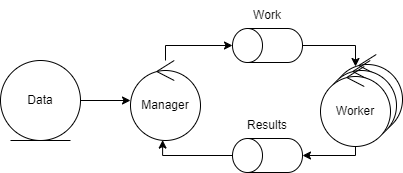
\includegraphics[scale=0.5]{resources/distributed_systems/grid_search_arch.png}
    \caption{Arquitectura de Grid Search}
    \label{fig:sis_dist:grid_search_arch}
\end{figure}

\newpage

\subsubsection{Pipeline Procesamiento de Imágenes} \label{sec:ip_desc}

En los últimos años, las redes neuronales profundas ganaron mucha popularidad gracias a su capacidad para resolver problemas complejos \cite{sis_dist:dnn}. Un conjunto de redes muy prometedor es el de las redes neuronales convolucionales, ampliamente utilizadas para el análisis de imágenes \cite{sis_dist:cnn}. Estas redes, por lo general, requieren valores de entrada normalizados, es decir, imágenes en un determinado formato, tamaño, etcétera. Como los \english{datasets} pueden llegar a ser muy grandes, puede ser beneficioso implementar este proceso de manera distribuida, a través de un \english{pipeline} de procesamiento.

Se plantea un sistema donde cada etapa realiza una transformación específica:
\begin{itemize}
    \item Formato: conversión al formato PNG \cite{sis_dist:png}.
    \item Resolución: reducción a una resolución de 100x100 píxeles.
    \item Tamaño: recortado del cuadrado central de 30x30 píxeles.
\end{itemize}

En la Figura \ref{fig:sis_dist:ip_example} se puede observar un ejemplo de cada una de estas etapas.

\begin{figure}[h]
    \centering
    \begin{subfigure}[b]{0.3\textwidth}
        \centering
        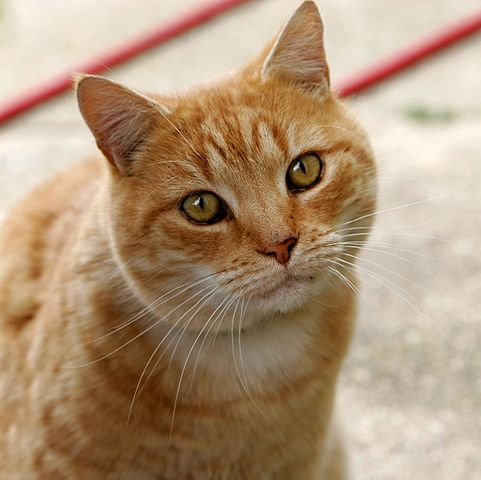
\includegraphics[width=\textwidth]{resources/distributed_systems/pipeline_images/input.jpg}
        \caption{Original}
    \end{subfigure}
    \hspace{10mm}
    \begin{subfigure}[b]{0.3\textwidth}
        \centering
        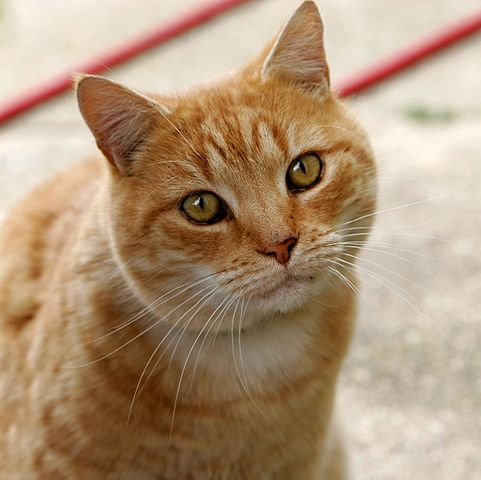
\includegraphics[width=\textwidth]{resources/distributed_systems/pipeline_images/formatted.png}
        \caption{Convertida a PNG}
    \end{subfigure}
    
    \begin{subfigure}[b]{0.3\textwidth}
        \centering
        
\includegraphics[width=\textwidth]{resources/distributed_systems/pipeline_images/scaled.png}
        \caption{Escalada a 100x100 píxeles}
    \end{subfigure}
    \hspace{10mm}
    \begin{subfigure}[b]{0.3\textwidth}
        \centering
        
\includegraphics[width=\textwidth]{resources/distributed_systems/pipeline_images/cropped.png}
        \caption{Recortada a 30x30 píxeles}
    \end{subfigure}
    \caption{Ejemplo de transformaciones del \english{pipeline} de procesamiento de imágenes}
    \label{fig:sis_dist:ip_example}
\end{figure}

La arquitectura está compuesta por un nodo \english{manager} y etapas de trabajadores para cada transformación. El trabajo es distribuido mediante colas, o herramientas similares. Las imágenes son accedidas mediante un sistema de archivos compartido (ver Figura~\ref{fig:sis_dist:image_processing_arch}).

\begin{figure}[h]
    \centering
    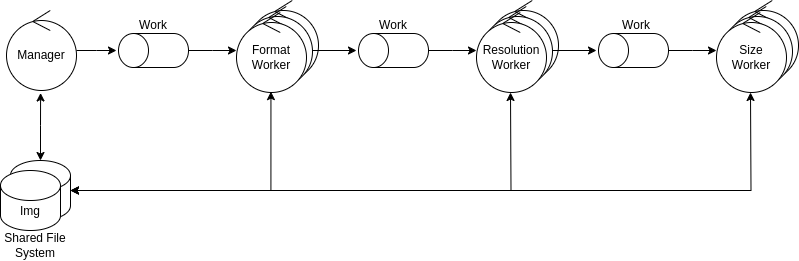
\includegraphics[scale=0.5]{resources/distributed_systems/image_processing_arch.png}
    \caption{Arquitectura de Procesamiento de Imágenes}
    \label{fig:sis_dist:image_processing_arch}
\end{figure}

\newpage

\subsection{Despliegue}

En esta sección se especifican los detalles de despliegue. Esto incluye los entornos de ejecución y datos utilizados.

\subsubsection{Entornos}

Debido a que FaMAF-1 se encontraba en uso durante el período de pruebas, los casos fueron ejecutados solamente en FaMAF-2. De esta manera, nos aseguramos de que las métricas tengan la menor interferencia posible con la ejecución de otros procesos.

Además, se realizaron ejecuciones complementarias en \english{Google Cloud Platform} (GCP), a modo de obtener mediciones comparativas en diferentes entornos. En particular, se utilizaron dos tipos de máquinas virtuales: el primero cuenta con un procesador Intel Cascade Lake o Ice Lake (sujeto a disponibilidad), dos vCPU (un único \english{hardware thread}), 8 GB de memoria RAM y disco SSD local; el segundo cuenta con un procesador Intel Skylake, Broadwell, Haswell, Sandy Bridge, o Ivy Bridge, 1 vCPU (un único \english{hardware thread}), $3.75$ GB de memoria RAM y disco SSD local\footnote{Para más información, el ambiente completo se encuentra detallado en formato de archivos de Terraform, disponible en \url{https://github.com/tpf-concurrent-benchmarks/gcp_deployment}}.

\subsubsection{Dataset}

Para la evaluación del Grid Search, se ejecutará la función Griewank \cite{sis_dist:griewank} dentro del rango \break
[-600; 600; $0.2$]\^{}3, es decir, el rango que va de -600 a 600 con paso de $0.2$ en 3 parámetros. Cada paquete (o \english{batch}) tiene un máximo de \numprint{10800000} números. El objetivo será buscar la configuración de parámetros que devuelven el mínimo resultado.

Para la evaluación del procesamiento de imágenes se utiliza el \english{dataset} BIRDS 525 SPECIES \cite{sis_dist:birds_dataset}. Con el fin de aumentar el tiempo de procesamiento total y, en consecuencia, mejorar la calidad de las métricas, se aplicaron una serie de transformaciones que duplicaron el tamaño del \english{dataset}\footnote{El script utilizado puede encontrarse en: \url{https://github.com/tpf-concurrent-benchmarks/various/blob/main/image_processing/image_multiplicator.py}. No se utilizaron las rotaciones.}, más específicamente, espejado vertical y horizontal de las imágenes.

\newpage

\subsection{Implementación}

En esta sección se desarrollan los detalles de implementación para cada lenguaje. Se incluyen diagramas con fin de explicar las particularidades de cada arquitectura, así como secciones de código que sean útiles para transmitir las características relevantes de los lenguajes y sus \english{frameworks}.

\subsubsection{C++}

Se seleccionó este lenguaje como \english{baseline} de comparación con otros lenguajes, ya que es un lenguaje clásico y de uso general que se utiliza en varias soluciones distribuidas \cite{cpp:ex:ray-io} \cite{cpp:ex:red-panda}.

Para la comunicación de procesos se utilizó ZMQ \cite{cpp:lib:zmq}, el cual provee colas de mensajería ligeras y adecuadas para este trabajo.

En cuanto a la implementación, se aprovecharon al máximo las capacidades que ofrece C++ al ser un lenguaje de programación de bajo nivel, como por ejemplo, la capacidad de asignar memoria manualmente, crear estructuras de datos compactas y eficientes y el uso de \english{templates}.

Adicionalmente, gracias a que ZMQ no hace uso de una instancia dedicada de \english{middleware} (es decir, no hay un nodo mediador centralizado) también se redujo mucho el costo adicional en comunicación.

En el caso del procesamiento de imágenes, al haber utilizado ZMQ, nos requirió crear procesos que actúan como un \english{broker}, como se puede ver en la Figura \ref{fig:cpp:image_processing_arch}. Es decir, procesos que actúan como intermediarios que permiten recibir mensajes de N procesos, y al mismo tiempo, enviar mensajes a N procesos bajo algún algoritmo (por ejemplo, \english{round-robin}).

\begin{figure}[ht]
    \centering
    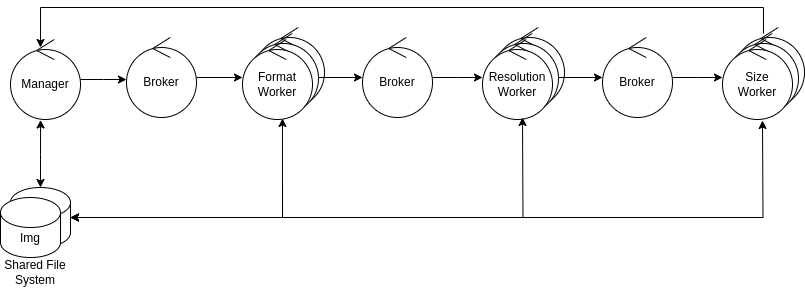
\includegraphics[scale=0.4]{resources/distributed_systems/cpp/image_processing_arch.png}
    \caption{Arquitectura de Procesamiento de Imágenes en C++}
    \label{fig:cpp:image_processing_arch}
\end{figure}

Estos procesos \english{broker} se limitan a recibir los mensajes de una etapa de \english{workers} y enviarlos a la siguiente, como podemos ver en el Código~\ref{code:cpp:broker}.

\begin{listing}[ht]
\begin{minted}[bgcolor=bg, breaklines]{c++}
int main()
{
    Protocol protocol(getPushPort(), getPullPort());
    bool shouldStop = false;

    while (!shouldStop)
    {
        std::string message = protocol.receive();
        if (message == Constants::STOP_MESSAGE)
        {
            shouldStop = true;
            continue;
        }
        protocol.send(message);
    }
    protocol.close();
}
\end{minted}
\caption{Función principal de un \english{broker} genérico en C++}
\label{code:cpp:broker}
\end{listing}

Por otro lado, el funcionamiento de los trabajadores es independiente de quién recibe los mensajes, pues la lógica de comunicación está abstraída de su función y es configurada por separado. Podemos ver el funcionamiento de uno de los \english{workers} en el Código~\ref{code:cpp:format_worker}.

\begin{listing}[ht]
\begin{minted}[bgcolor=bg, breaklines]{c++}
while (!shouldStop)
{
    std::string message = protocol.receive();
    if (message == Constants::STOP_MESSAGE)
    {
        shouldStop = true;
    }
    else
    {
        std::string imageName = message.substr(message.find_last_of('/') + 1);
        std::string newImageName = imageName.substr(0, imageName.find_last_of('.')) + ".png";

        std::chrono::milliseconds start_time_ms = std::chrono::duration_cast<std::chrono::milliseconds>(
            std::chrono::system_clock::now().time_since_epoch());

        change_format(message, "../../shared_vol/formatted/" + newImageName);

        std::chrono::milliseconds end_time_ms = std::chrono::duration_cast<std::chrono::milliseconds>(
            std::chrono::system_clock::now().time_since_epoch());
        std::chrono::milliseconds completion_time = end_time_ms - start_time_ms;
        statsdClient.timing("work_time", completion_time.count(), 1);
        statsdClient.increment("results_produced");

        protocol.send("../../shared_vol/formatted/" + newImageName);
    }
}
\end{minted}
\caption{Extracto de la función principal de un \english{format worker} en C++}
\label{code:cpp:format_worker}
\end{listing}

Adicionalmente, se debió implementar polling sobre dos tipos \english{sockets} en simultáneo (ver Código~\ref{code:cpp:polling}). Se utiliza un \english{socket push-pull} para el envío equitativo de tareas. Y se utiliza un \english{socket pub-sub} para los mensajes al finalizar el procesamiento.

\begin{listing}[ht]
\begin{minted}[bgcolor=bg, breaklines]{c++}
std::string Protocol::receive()
{
    zmq::pollitem_t items[] = {
            {receiver_, 0, ZMQ_POLLIN, 0},
            {end_work_, 0, ZMQ_POLLIN, 0}};
    zmq::poll(&items[0], 2, -1);

    if (items[0].revents & ZMQ_POLLIN)
    {
        zmq::message_t message;
        const zmq::recv_result_t &anOptional = receiver_.recv(message);
        if (!anOptional.has_value())
        {
            return "Error message";
        }
        return std::string(static_cast<char *>(message.data()), message.size());
    }
    else if (items[1].revents & ZMQ_POLLIN)
    {
        zmq::message_t message;
        const zmq::recv_result_t &anOptional = end_work_.recv(message);
        if (!anOptional.has_value())
        {
            return "Error message";
        }
        return std::string(static_cast<char *>(message.data()), message.size());
    }
    else
    {
        return "Error message";
    }
}
\end{minted}
\caption{Extracto de la función principal de un \english{format worker} en C++}
\label{code:cpp:polling}
\end{listing}

\subsubsection{Scala}

Se seleccionó este lenguaje porque es utilizado para el desarrollo de herramientas de procesamiento distribuido populares, como Apache Spark \cite{scala:ex:spark}; reflejando el estándar de la industria para esta área.

Se utilizó RabbitMQ \cite{scala:lib:rabbit} como \english{middleware} para la distribución de trabajo, el cual requiere un \english{broker} centralizado en el cual se definirán las colas de comunicación. Podemos ver en la Figura~\ref{fig:scala:image_processing_arch} la arquitectura del \english{pipeline} de imágenes, donde se aprecia que los componentes se encuentran conectados únicamente con el \english{broker} de RabbitMQ. El flujo de datos y la arquitectura es igual a los definidos en la Figura~\ref{fig:sis_dist:image_processing_arch}, pero el manejo de todas las colas es mediante este \english{broker}.

\begin{figure}[ht]
    \centering
    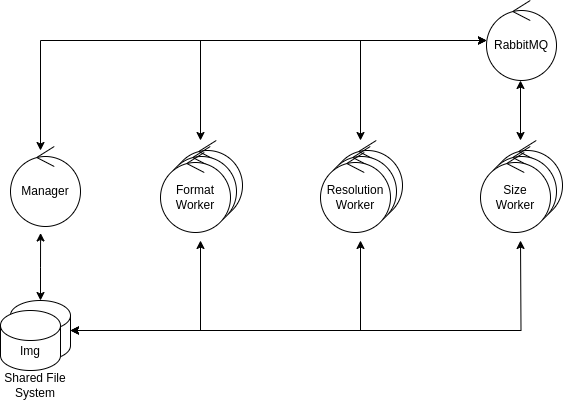
\includegraphics[scale=0.4]{resources/distributed_systems/scala/image_processing_arch.png}
    \caption{Arquitectura de Procesamiento de Imágenes en Scala}
    \label{fig:scala:image_processing_arch}
\end{figure}

Se intentó utilizar Akka \cite{scala:lib:akka}, un \english{framework} popular para sistemas distribuidos basado en actores, pero su uso resultó ser dificultoso y se descartó en pos de mantener el cronograma.

Se aprovecharon ampliamente las herramientas del lenguaje para evaluación perezosa\footnote{Evaluación perezosa: Estrategia de evaluación de una función o método, que implica retrasar la evaluación hasta el momento en que el resultado es requerido.} de iteradores. En el Código~\ref{code:scala:split} se puede observar el método que genera las particiones de trabajo de manera perezosa para la búsqueda en grilla.

\begin{listing}[ht]
\begin{minted}[bgcolor=bg, breaklines]{scala}
def split(maxChunkSize: Int, precision: Option[Int] = None): Iterator[Work] = {
    val minBatches = Math.ceil(size.toDouble / maxChunkSize)
    val partitionsPerInterval = calcPartitionsPerInterval(minBatches.toInt)

    val listOfIterator = for (intervalPos <- intervals.indices) yield {
        val iterator = intervals(intervalPos).split(partitionsPerInterval(intervalPos), precision)
        CircularIterator(iterator, partitionsPerInterval(intervalPos), precision)
    }
    WorkPlan(listOfIterator.toList,aggregator).iterator
}
\end{minted}
\caption{Fragmento de métodos relacionados a la división de trabajo en Scala, correspondientes al caso de uso de Grid Search}
\label{code:scala:split}
\end{listing}

Otra herramienta que se aprovechó fue el uso de \english{Traits}\footnote{\english{Trait}: Conjunto de métodos que puede implementar una clase para definir su comportamiento.}, que permiten abstraer lógica común. En el Código~\ref{code:scala:basic_transformer} es posible apreciar la definición del \english{Trait} \lstinline{BasicTransformer} que encapsula la lógica de comunicación que utilizan todos los \english{workers} del \english{pipeline} de procesamiento de imágenes. Es interesante destacar que, gracias al nivel de abstracción del \english{Trait}, también fue posible utilizarlo en el caso de uso de Grid Search.

\begin{listing}[h]
\begin{minted}[bgcolor=bg, breaklines]{scala}
trait BasicTransformer {
    val inputQueue: String
    val outputQueue: String
    val endEvent: String
    type InputType
    type OutputType
    implicit val reader: Reader[InputType]
    implicit val writer: Writer[OutputType]

    def transform(input: InputType): Option[OutputType]

    private def setUpConsumer(middleware: MessageQueue): Unit = {
        middleware.setConsumer(inputQueue, input => {
            val convertedInput = read[InputType](input)

            val output = transform(convertedInput)
            output.foreach(o => {
                val outputString = default.write(o)
                middleware.produce(outputQueue, outputString.getBytes("UTF-8"))
            })
            true
        })
    }

    def start(middleware: MessageQueue): Unit = {
        setUpConsumer(middleware)
        val stopPromise = Promise[Unit]()

        middleware.subscribe(endEvent, end => {
            println(s"Received end: ${new String(end, "UTF-8")}")
            stopPromise.success(())
            true
        })
        println("Starting to consume")
        middleware.startConsuming(Some(stopPromise.future))
        middleware.close()
    }
}
\end{minted}
\caption{\english{Trait} utilizado para encapsular la lógica de comunicación común a los nodos trabajadores, utilizado en ambos casos de uso}
\label{code:scala:basic_transformer}
\end{listing}

En el Código~\ref{code:scala:resolution_worker} podemos ver la implementación del \english{resolution worker}, donde solo es necesaria la función de transformación de imagen y la lógica de comunicación, sincronización y \english{logging} están abstraídas.

\begin{listing}[h]
\begin{minted}[bgcolor=bg, breaklines]{scala}
case class ResolutionWorker(inputQueue: String,
                            outputQueue: String,
                            endEvent: String,
                            targetWidth: Int,
                            targetHeight: Int) extends BasicTransformer {
    override type InputType = FileName
    override type OutputType = FileName

    override implicit val reader: default.Reader[InputType] = fileNameRW
    override implicit val writer: default.Writer[OutputType] = fileNameRW

    override def transform(input: InputType): Option[OutputType] = {
        val sourcePath = input.path
        val sourceName = input.name
        val sourceFileName = s"$sourcePath/$sourceName"

        val targetPath = "./shared/scaled"
        val targetFileName = s"$targetPath/$sourceName"

        try {
            ImageUtils.scale(sourceFileName, targetFileName, targetWidth, targetHeight, ImageFormat.Png())
            Some(FileName(targetPath, sourceName))
        } catch {
            case e: java.io.FileNotFoundException =>
                println(s"Input file $sourceFileName not found - skipping")
                None
        }
    }
}
\end{minted}
\caption{Implementación de \english{resolution worker} en Scala}
\label{code:scala:resolution_worker}
\end{listing}

\subsubsection{Go}

Si bien sus aplicaciones en sistemas distribuidos son aún jóvenes, Go está tomando popularidad en este ámbito, y han surgido proyectos interesantes en los últimos tiempos \cite{go:ex:awesome-go}. Esto lo convierte en un buen lenguaje para comparar.

Para la comunicación entre sistemas se utilizó NATS \cite{go:lib:nats}, un \english{middleware} orientado a los mensajes desarrollado en Go. Al igual que RabbitMQ, hace uso de una instancia intermedia para la entrega de mensajes que provee persistencia, tolerancia a fallas y balanceo de carga. Podemos ver la adaptación de la arquitectura del \english{pipeline} de procesamiento de imágenes en la Figura~\ref{fig:go:image_processing_arch}.

\begin{figure}[ht]
    \centering
    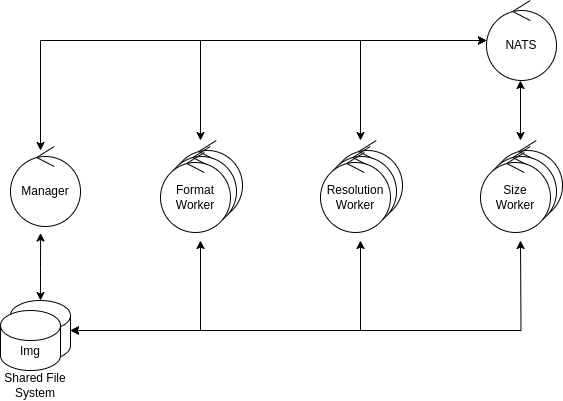
\includegraphics[scale=0.4]{resources/distributed_systems/go/image_processing_arch.png}
    \caption{Arquitectura de Procesamiento de Imágenes en Go}
    \label{fig:go:image_processing_arch}
\end{figure}

Se empleó el modelo de publicador y suscriptor provisto por el \english{middleware}, en el cual los trabajadores se suscriben a una cola para recibir el trabajo. Es posible observar, en el Código~\ref{code:go:size_worker}, la lógica principal del \english{size worker} en el \english{pipeline} de imágenes, donde se realiza la suscripción a la cola de entrada y la definición de la función \english{callback} que será ejecutada al recibir un mensaje.

\begin{listing}[ht]
\begin{minted}[bgcolor=bg, breaklines]{go}
func subscribeForWork(conn *nats.Conn, workerConfig config.Config, statsdClient statsd.Statter) {
	_, err := conn.QueueSubscribe(workerConfig.Queues.Input, "workers_group", func(msg *nats.Msg) {
		imagePath := string(msg.Data)
		newImagePath := createOutputDir(imagePath)

		startTime := time.Now()

		image_processing.CropCentered(imagePath, newImagePath, workerConfig.Worker.TargetWidth, workerConfig.Worker.TargetHeight)

		endTime := time.Now()
		elapseTime := endTime.Sub(startTime).Milliseconds()
		err := statsdClient.Timing("work_time", elapseTime, 1.0)
		if err != nil {
			log.Fatalf("Error sending metric to statsd: %s", err)
		}

		err = statsdClient.Inc("results_produced", 1, 1.0)
		if err != nil {
			log.Fatalf("Error sending metric to statsd: %s", err)
		}

		err = conn.Publish(workerConfig.Queues.Output, []byte(common.JobDoneMessage))
		if err != nil {
			log.Fatalf("Error publishing to queue: %s", err)
		}
	})
	if err != nil {
		log.Fatalf("Error subscribing to queue: %s", err)
	}
}
\end{minted}
\caption{Fragmento de \english{size worker} en Go}
\label{code:go:size_worker}
\end{listing}

Se usaron \english{structs} para representar los datos y se siguió el paradigma imperativo procedural para implementar el comportamiento. En el Código~\ref{code:go:grid_search} se aprecia la implementación principal de los \english{workers} de Grid Search, donde la información es almacenada en el \english{struct} \lstinline{GridSearch}, cuyo metodo \lstinline{Search} iterará la grilla y acumulará los resultados al ejecutar la función.

\begin{listing}[ht]
\begin{minted}[bgcolor=bg, breaklines]{go}
type GridSearch struct {
	params      *Params
	result      float64
	totalInputs uint64
	accumType   string
	input       [Size]float64
}

func (gs *GridSearch) Search(callback func([Size]float64) float64) {
	accumulator := NewAccumulator(gs.accumType)

	for i := int64(0); i < gs.params.getTotalIterations(); i++ {
		params := gs.params.getCurrent()
		result := callback(params)
		accumulator.Accumulate(result, params)
		gs.params.next()
	}
	gs.result = accumulator.GetResult()
	gs.input = accumulator.GetInput()
}
\end{minted}
\caption{Lógica principal de \english{worker} de Grid Search en Go}
\label{code:go:grid_search}
\end{listing}


\subsubsection{Julia}

Se seleccionó este lenguaje debido a que posee una biblioteca nativa para procesamiento distribuido \cite{jl:lib:distributed}, lo cual sugiere la idoneidad del lenguaje en este dominio de aplicación.

El uso de esta biblioteca permite definir una arquitectura maestro-esclavo, donde los trabajadores se registran con el \english{manager}, quien se encarga de distribuir y coordinar los procesos. En la Figura~\ref{fig:jl:image_processing_arch} se muestra la adaptación de la arquitectura del \english{pipeline} de procesamiento de imágenes. Como se puede ver, la comunicación entre procesos se da por medio del \english{manager}.

\begin{figure}[ht]
    \centering
    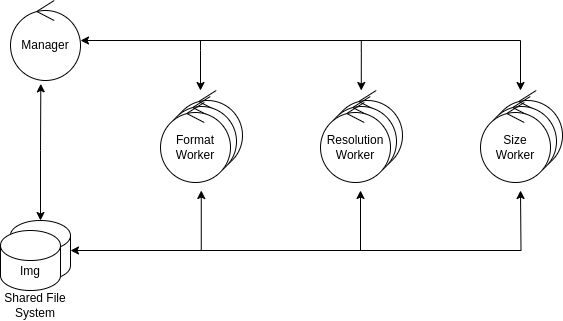
\includegraphics[scale=0.4]{resources/distributed_systems/jl/image_processing_arch.png}
    \caption{Arquitectura de Procesamiento de Imágenes en Julia}
    \label{fig:jl:image_processing_arch}
\end{figure}

En específico, para la implementación de Grid Search se empleó la capacidad nativa de ejecutar un \lstinline{map} en un conjunto (\english{pool}) de trabajadores. La biblioteca brinda un elevado nivel de abstracción, pues estos trabajadores pueden encontrarse en la misma computadora o no. En el Código~\ref{code:jl:pmap} se observa el empleo de la función \lstinline{pmap}, que ejecuta una función en un conjunto de trabajadores; y el decorador \lstinline{@everywhere}, que permite especificar las secciones de código que se definirán en todos los contextos. Esto último se requiere debido a que los nodos trabajadores pueden inicializarse sin conocer el código con anticipación. El nodo \english{manager} le comunicará a los trabajadores aquellas secciones de código marcadas con el decorador.

\begin{listing}[ht]
\begin{minted}[bgcolor=bg, breaklines]{julia}
@everywhere function evaluate_for_partition(sub_work_partition)
    map(sub_work_partition) do sub_work
        res = StatsLogger.runAndMeasure("work_time") do
            Works.evaluate_for!(sub_work, VALUES, RESULTS)
        end
        StatsLogger.increment("results_produced")
        return res
    end
end

function distribute_work(sub_works_parts, pool)
    @showprogress pmap(pool, sub_works_parts) do sub_work_partition
        evaluate_for_partition(sub_work_partition)
    end
end
\end{minted}
\caption{Distribución de tareas de Grid Search en Julia}
\label{code:jl:pmap}
\end{listing}

Para el caso de procesamiento de imágenes se emplearon canales remotos como colas de tareas. Éstos se encuentran definidos en el nodo \english{manager}, que cumple la función \english{broker}. En el Código~\ref{code:jl:channels} se muestra la definición de estos canales, y en el Código~\ref{code:jl:pipeline} la definición del \english{pipeline}. 
De esta manera, tanto la arquitectura, como los canales de comunicación y la funcionalidad de los trabajadores, están definidos por código en el nodo \english{manager}.

\begin{listing}[ht]
\begin{minted}[bgcolor=bg, breaklines]{julia}
format_channel = RemoteChannel(()->Channel{String}(32))
resolution_channel = RemoteChannel(()->Channel{String}(32))
size_channel = RemoteChannel(()->Channel{String}(32))
result_channel = RemoteChannel(()->Channel{String}(32))

close_channels = () -> for chan in [format_channel, resolution_channel, size_channel, result_channel]
    close(chan)
end
get_channels() = format_channel, resolution_channel, size_channel, result_channel, close_channels
\end{minted}
\caption{Creación de canales remotos en Julia}
\label{code:jl:channels}
\end{listing}

\begin{listing}[ht]
\begin{minted}[bgcolor=bg, breaklines]{julia}
function start_worker_stage( workers::Array, handler::Function, in_channel::RemoteChannel, out_channel::RemoteChannel, type="worker" )
    for (i, p) in enumerate(workers)
        remote_do( worker_loop, p, handler, in_channel, out_channel, string(type, ".", i-1) )
    end
end

function start_pipeline()
    println("Starting workers")
    format_channel, resolution_channel, size_channel, result_channel = get_channels()
    format_workers, resolution_workers, size_workers = get_workers()

    # Start Format workers
    start_worker_stage( format_workers, format_handler, format_channel, resolution_channel, "format" )
    
    # Start Resolution workers
    start_worker_stage( resolution_workers, resolution_handler, resolution_channel, size_channel, "resolution" )
    
    # Start Size workers
    start_worker_stage( size_workers, size_handler, size_channel, result_channel, "size" )

    return format_channel, result_channel
end
\end{minted}
\caption{Definición del \english{pipeline} de procesamiento de imágenes en Julia}
\label{code:jl:pipeline}
\end{listing}

\subsubsection{Elixir}

La máquina virtual de Erlang es muy utilizada para sistemas distribuidos \cite{elx:ex:companies} \cite{scala:lib:rabbit}. Elixir nos permite comparar ese entorno y su sistema de actores mediante una interfaz más moderna, lo cual nos llevó a seleccionar este lenguaje para comparar.

Se creó un \english{framework} de procesamiento distribuido basado en las herramientas de actores distribuidos nativas, debido a que no se encontraron herramientas externas que cumplieran con las especificaciones requeridas. Puede encontrarse la especificación del \english{framework} en los repositorios o en la documentación \cite{repos:docs}.

Se puede observar, en la Figura~\ref{fig:elx:image_processing_framework}, la definición de procesos del \english{pipeline} de procesamiento de imágenes utilizando el \english{framework} mencionado. Se definen cuatro tipos de nodo:
\begin{enumerate}
\item Fuente (\english{Source}): ingresa los datos al sistema, que serán posteriormente enviados a la primera etapa de trabajadores.
    \item Trabajador (\english{Worker}): realiza el procesamiento, recibiendo datos de una fuente y enviando los resultados a un sumidero.
    \item Mediador (\english{Broker}): puede cumplir la función origen y destino desde el punto de vista del trabajador, repartiendo tareas entre etapas de trabajadores.
    \item  Sumidero (\english{Sink}): recibe los resultados al final del \english{pipeline}
\end{enumerate}

\begin{figure}[ht]
    \centering
    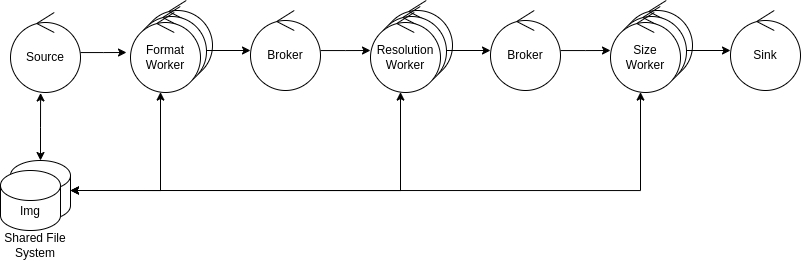
\includegraphics[scale=0.4]{resources/distributed_systems/elixir/image_processing_framework.png}
    \caption{Procesos de Procesamiento de Imágenes en Elixir}
    \label{fig:elx:image_processing_framework}
\end{figure}

Por otro lado, se puede ver en la Figura~\ref{fig:elx:image_processing_arch} el despliegue real del sistema, donde los procesos \english{source}, \english{sink} y \english{broker} son ejecutados dentro del nodo \english{manager}.

\begin{figure}[ht]
    \centering
    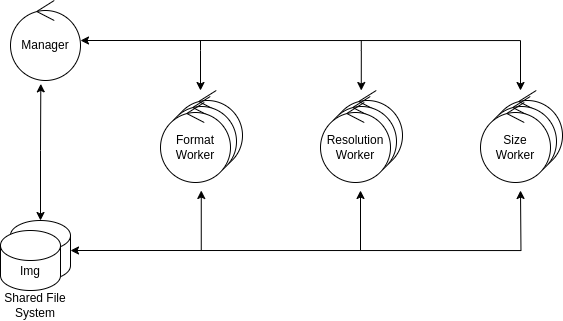
\includegraphics[scale=0.4]{resources/distributed_systems/elixir/image_processing_arch.png}
    \caption{Arquitectura de Procesamiento de Imágenes en Elixir}
    \label{fig:elx:image_processing_arch}
\end{figure}

Al igual que en Julia, el código está completamente definido sobre el nodo \english{manager}. Este es este quien asigna la funcionalidad de los trabajadores, además de proveerles el trabajo. Podemos observar la definición del sistema para Grid Search en el Código~\ref{code:elx:gs} y para el \english{pipeline} de imágenes en el Código~\ref{code:elx:ip}. El método \lstinline{start_link} es el que instancia a los actores locales del \english{source}, \english{sink} y \english{broker}; mientras que los trabajadores remotos son iniciados mediante \lstinline{start_remote_worker}.

\begin{listing}[ht]
\begin{minted}[bgcolor=bg, breaklines]{elixir}
def distributed_gs do
    config = ConfigReader.get_config("/app/lib/resources/data.json", :manager)
    IO.puts("Config read: #{inspect(config)}")
    data = Enum.at(config["data"], 0)
    data2 = Enum.at(config["data"], 1)
    data3 = Enum.at(config["data"], 2)
    interval = Interval.newInterval(Enum.at(data, 0), Enum.at(data, 1), Enum.at(data, 2))
    interval2 = Interval.newInterval(Enum.at(data2, 0), Enum.at(data2, 1), Enum.at(data2, 2))
    interval3 = Interval.newInterval(Enum.at(data3, 0), Enum.at(data3, 1), Enum.at(data3, 2))
    
    partition = Partition.newPartition([interval, interval2, interval3], 3, config["maxItemsPerBatch"])
    {:ok, source} = WorkSource.start_link(partition, config["agg"])
    IO.puts("Source pid: #{inspect(source)}")
    {:ok, sink} = WorkSink.start_link()
    IO.puts("Sink pid: #{inspect(sink)}")
    
    workers_replicas = String.to_integer(System.get_env("WORKER_REPLICAS"))
    
    workers =
        Enum.map(1..workers_replicas, fn num ->
            {:ok, pid} = start_remote_worker(GridSearchWorker, source, sink, num)
            GenServer.cast(pid, :start)
            pid
        end)
    
    cleanup(source, workers, [], sink)
end
\end{minted}
\caption{Definición del \english{pipeline} para Grid Search en Elixir}
\label{code:elx:gs}
\end{listing}

\begin{listing}[ht]
\begin{minted}[bgcolor=bg, breaklines]{elixir}
def distributed_ip do
    {:ok, source} = WorkSource.start_link("shared/input", 25)
    IO.puts "Source pid: #{inspect source}"
    {:ok, sink} = WorkSink.start_link()
    IO.puts "Sink pid: #{inspect sink}"
    {:ok, broker_1} = WorkBroker.start_link()
    IO.puts "Broker 1 pid: #{inspect broker_1}"
    {:ok, broker_2} = WorkBroker.start_link()
    IO.puts "Broker 2 pid: #{inspect broker_2}"
    
    
    format_workers_replicas = String.to_integer(System.get_env("FORMAT_WORKER_REPLICAS"))
    stage_1_workers = Enum.map(1..format_workers_replicas, fn num ->
        {:ok, pid} = start_remote_worker(FormatWorker, source, broker_1, num)
        GenServer.cast(pid, :start)
        pid
    end)
    
    resolution_workers_replicas = String.to_integer(System.get_env("RESOLUTION_WORKER_REPLICAS"))
    stage_2_workers = Enum.map(1..resolution_workers_replicas, fn num ->
        {:ok, pid} = start_remote_worker(ResolutionWorker, broker_1, broker_2, num)
        GenServer.cast(pid, :start)
        pid
    end)
    
    size_workers_replicas = String.to_integer(System.get_env("SIZE_WORKER_REPLICAS"))
    stage_3_workers = Enum.map(1..size_workers_replicas, fn num ->
        {:ok, pid} = start_remote_worker(SizeWorker, broker_2, sink, num)
        GenServer.cast(pid, :start)
        pid
    end)
    
    workers = stage_1_workers ++ stage_2_workers ++ stage_3_workers
    
    cleanup(source, workers, [broker_1, broker_2], sink)
end
\end{minted}
\caption{Método de inicialización de \english{workers} remotos del \english{pipeline} de procesamiento de imágenes en Elixir}
\label{code:elx:ip}
\end{listing}

El método \lstinline{start_remote_worker} (ver Código~\ref{code:elx:start_worker}) hace uso de las herramientas nativas del lenguaje para desplegar código en un nodo remoto. Debido a limitaciones del lenguaje, es necesario definir un método \english{proxy} para poder instanciar el actor deseado.

\begin{listing}[ht]
\begin{minted}[bgcolor=bg, breaklines]{elixir}
def start_worker_proxy(worker_type, source, sink) do
    {:ok, worker_pid} = MeasuredBatchedWorker.start_link(worker_type, source, sink)
    
    # Send worker_pid when asked for it
    receive do
        {:pid_req, ref} ->
            send ref, {:pid_res, worker_pid}
    end
    
    Utils.wait_for_process(worker_pid)
    {:ok, worker_pid}
end

def start_remote_worker(worker_type, source, sink, num) do
    remote = String.to_atom("worker@#{worker_type.name()}_worker_#{num}")
    IO.puts "Remote: #{inspect remote}"
    proxy_pid = Node.spawn_link(remote, DistributedPipeline, :start_worker_proxy, [worker_type, source, sink])
    IO.puts "Proxy pid: #{inspect proxy_pid}"
    
    # Request the pid of the worker from the proxy on the Node
    send proxy_pid, {:pid_req, self()}
    receive do
        {:pid_res, worker_pid} ->
            {:ok, worker_pid}
    end
end
\end{minted}
\caption{Definición del \english{pipeline} de procesamiento de imágenes en Elixir}
\label{code:elx:start_worker}
\end{listing}

El lenguaje, al ser completamente funcional, no permite la mutación de estructuras de datos, lo cual no fue muy compatible con el caso uso de Grid Search, donde se podía aprovechar la reutilización de estructuras.

\subsection{Métricas}

A continuación se realiza un análisis abreviado de las métricas efectuadas, para ambos casos de uso.
La totalidad de las métricas puede encontrarse en la sección~\ref{sec:anex:metrics} (\nameref{sec:anex:metrics}). Específicamente \ref{sec:anex:metrics:gs} (\nameref{sec:anex:metrics:gs}) y \ref{sec:anex:metrics:ip} (\nameref{sec:anex:metrics:ip}).

\subsubsection{Despliegue - Grid Search} \label{sec:gs_metrics}

En el Cuadro~\ref{tab:sis_dist:gs_metrics} se pueden observar los resultados correspondientes al primer caso de uso. El significado de cada una de las métricas es el siguiente:

\begin{itemize}
    \item \textbf{\english{Throughput} combinado}: tasa de datos procesados por unidad de tiempo.
    \item \textbf{Uso de memoria}: uso de memoria promedio de los procesos trabajadores.
    \item \textbf{Uso de red}: uso de red promedio de los procesos trabajadores.
\end{itemize}

Este resumen se encuentra expresado en valores relativos a C++. Esto quiere decir, por ejemplo, que el \english{Throughput} de Scala fue el 27\% del Throughput de C++.

\begin{table}[h]
\centering
\begin{tabular}{|l|l|l|l|l|l|}
\hline
\multicolumn{1}{|c|}{Métrica} & \multicolumn{1}{c|}{C++} & \multicolumn{1}{c|}{Scala} & \multicolumn{1}{c|}{Go} & \multicolumn{1}{c|}{Julia} & \multicolumn{1}{c|}{Elixir} \\ \hline
\english{Throughput} combinado           & 100\%                    & 27\%                       & 80\%                    & 55\%                       & 10\%                        \\ \hline
Uso de memoria                  & 100\%                    & \numprint{9175}\%                     & 175\%                   & \numprint{31744}\%                    & \numprint{2250}\%                      \\ \hline
Uso de red                 & 100\%                    & 60\%                       & 84\%                    & 59\%                       & 80\%                        \\ \hline
\end{tabular}
\caption{Resumen de métricas de Grid Search. Basado en mediciones para 8 nodos trabajadores, ejecutadas en FaMAF-2, relativas a C++ (Ver Cuadro \ref{tab:gs:8_workers_famaf2})}
\label{tab:sis_dist:gs_metrics}
\end{table}

Algunos datos interesantes que se pueden extraer de estos valores, son los siguientes:

\begin{itemize}
    \item C++ y Go son más veloces que el resto de lenguajes, y utilizan menos memoria: esto se debe, probablemente, a que se trata de los únicos lenguajes compilados que se analizaron.
    \item Julia utiliza mucha memoria para este caso (más de 1 GB por \english{Worker}): para evitar que el intérprete realice asignaciones de memoria innecesarias en ciertas secciones del código, se debió reservar una gran cantidad de memoria al inicio del programa y reutilizarla constantemente. Esto puede haber ocasionado un aumento sustancial del uso de memoria de Julia. Ver uso de memoria en tabla \ref{tab:jl:gs:famaf2} (\nameref{tab:jl:gs:famaf2}).
    \item Scala es más lento de lo esperado: si bien no se trata de un lenguaje compilado, la madurez del ecosistema Java parecía brindar la posibilidad de una implementación con un mejor desempeño. Scala provee un elevado nivel de expresividad, pero esto tuvo su costo en el \english{Throughput}.
\end{itemize}

\subsubsection{Despliegue - Procesamiento de Imágenes}

En el Cuadro \ref{tab:sis_dist:ip_metrics} se pueden observar los resultados correspondientes al segundo caso de uso. El significado de cada una de las métricas es el siguiente:

\begin{itemize}
    \item \textbf{\english{Throughput} combinado}: la tasa de datos procesados por unidad de tiempo.
    \item \textbf{Uso de memoria máximo}: uso de memoria de los procesos trabajadores de la etapa con mayor uso.
    \item \textbf{Uso de red máximo}: uso de red de los procesos trabajadores de la etapa con mayor uso.
    \item \textbf{Uso de CPU promedio}: uso de CPU promedio de todos los trabajadores.
\end{itemize}

Este resumen, al igual que el Cuadro \ref{tab:sis_dist:gs_metrics}, está expresado en valores relativos a C++.

\begin{table}[h]
\centering
\begin{tabular}{|l|l|l|l|l|l|}
\hline
\multicolumn{1}{|c|}{Métrica} & \multicolumn{1}{c|}{C++} & \multicolumn{1}{c|}{Scala} & \multicolumn{1}{c|}{Go} & \multicolumn{1}{c|}{Julia} & \multicolumn{1}{c|}{Elixir} \\ \hline
\english{Throughput} combinado           & 100\%                    & 56\%                       & 37\%                    & 298\%                      & 56\%                        \\ \hline
Uso de memoria máximo              & 100\%                    & \numprint{1300}\%                     & 173\%                   & 836\%                      & 209\%                       \\ \hline
Uso de red máximo             & 100\%                    & 76\%                       & 34\%                    & 515\%                      & 33\%                        \\ \hline
Uso de CPU promedio                 & 100\%                    & 82\%                       & 160\%                   & 157\%                      & 156\%                       \\ \hline
\end{tabular}
\caption{Resumen de métricas de Procesamiento de Imágenes. Basado en mediciones para 4 nodos trabajadores por etapa, ejecutadas en FaMAF-2, relativas a C++ (Ver Cuadro \ref{tab:ip:4_workers_famaf_2})}
\label{tab:sis_dist:ip_metrics}
\end{table}

De estos datos, es posible obtener algunas conclusiones preliminares:

\begin{itemize}
    \item El rendimiento de Julia es marcadamente mejor para este caso de uso: tanto el \english{Throughput} como el uso de CPU son más altos que casi todos los otros lenguajes.
    \item El rendimiento de Elixir es mejor en comparación con el anterior caso de uso: Esto es debido a que en este caso las variables inmutables no son la mayor limitación, por lo que la \english{performance} se vuelve comparable a otros lenguajes.
\end{itemize}

\subsubsection{Generales} \label{sec:general_metrics}

Se evaluaron, además, algunas métricas aplicables a ambos casos de uso, a saber:

\begin{itemize}
    \item Tiempo: tiempo que tomaron los desarrollos relativo al planificado (4 semanas cada uno).
    \item Espacio: espacio que ocupan las imágenes de Docker en relación a la imagen base (alpine \cite{metrics:apline}). Unificados dado que la diferencia entre tipo de nodo (\english{manager}/\english{worker}/\english{middleware}) y caso (Grid Search, Procesamiento de Imágenes) es despreciable\footnote{Julia es la excepción, siendo que no pudo ser ejecutada en la imagen de alpine y tiene una amplia diferencia de tamaño según el caso de uso.}
\end{itemize}

Los resultados se pueden observar en la tabla \ref{tab:sis_dist:general_metrics}, elaborada a partir de las tablas \ref{tab:gs:image_sizes} y \ref{tab:ip:image_sizes}.

\begin{table}
\centering
\begin{tabular}{|l|l|l|l|l|l|}
\hline
\multicolumn{1}{|c|}{Métrica} & \multicolumn{1}{c|}{C++} & \multicolumn{1}{c|}{Scala} & \multicolumn{1}{c|}{Go} & \multicolumn{1}{c|}{Julia} & \multicolumn{1}{c|}{Elixir} \\ \hline
Tiempo                        & 125\%                    & 100\%                      & 75\%                    & 50\%                       & 150\%                       \\ \hline
Espacio                       & x2.5                     & x26.2                      & x2                      & x100-x266                  & x11.4                       \\ \hline
\end{tabular}
\caption{Métricas generales correspondientes al área de Sistemas Distribuidos}
\label{tab:sis_dist:general_metrics}
\end{table}

\subsection{Experiencias}

Se realizó una evaluación subjetiva de los lenguajes de programación según nuestra experiencia desarrollando con ellos.

\subsubsection{Comparación} \label{sec:subjective_comparison}

Los atributos que se tuvieron en cuenta a la hora de realizar la comparación entre lenguajes, son los siguientes:

\begin{itemize}
    \item \textbf{Expresividad}: capacidad de expresar soluciones a problemas complejos de forma adecuada, simple y concisa.
    \item \textbf{Simplicidad}: qué tan fácil es aprender, utilizar e interpretar el lenguaje.
    \item \textbf{Manejo de memoria}: herramientas que proveen el lenguaje para manejar memoria, su simplicidad de uso y la capacidad de administrarla.
    \item \textbf{Manejo de errores}: herramientas que provee el lenguaje para manejar errores, su simplicidad de uso, la expresividad de los errores.
    \item \textbf{Manejo de concurrencia}: herramientas que provee el lenguaje para aplicar concurrencia, su simplicidad de uso y efectividad.
    \item \textbf{Manejo de bibliotecas}: sistema de bibliotecas y módulos que provee el lenguaje. Eficacia de su gestor de paquetes (si tiene). Disponibilidad y calidad de recursos.
\end{itemize}

Para cada atributo y lenguaje se asignó un puntaje de 1 a 5, donde 1 significa que el lenguaje destaca muy negativamente en ese atributo, y 5 significa que el lenguaje destaca muy positivamente. Los resultados se observan en el Cuadro \ref{tab:sis_dist:experiences}

\begin{table}[h]
\centering
\begin{tabular}{|l|c|c|c|c|c|}
\hline
\multicolumn{1}{|c|}{Atributo} & C++ & Scala & Go & Julia & Elixir \\ \hline
Expresividad & \badMetric{2} & \goodMetric{4} & 3 & \goodMetric{4} & \badMetric{1} \\ \hline
Simplicidad & 3 & \goodMetric{4} & \goodMetric{5} & 3 & \badMetric{2} \\ \hline
Memoria & \goodMetric{4} & 3 & \goodMetric{4} & 3 & 3 \\ \hline
Errores & \badMetric{2} & 3 & 3 & 3 & \badMetric{1} \\ \hline
Concurrencia & \badMetric{2} & \goodMetric{5} & \goodMetric{5} & \goodMetric{5} & \goodMetric{5} \\ \hline
Bibliotecas & \badMetric{1} & \goodMetric{4} & \goodMetric{5} & \goodMetric{4} & \badMetric{2} \\ \hline
\end{tabular}
\caption{Resumen de la comparación de atributos para el área de Sistemas Distribuidos}
\label{tab:sis_dist:experiences}
\end{table}

\subsubsection{C++}

El desarrollo de este caso no fue sencillo, ya que el control adicional que ofrece C++ sobre el programa incrementa significativamente la complejidad de la programación, lo que resultó en un mayor tiempo de desarrollo de este caso en comparación con otras. Conceptos como RAII (\textit{Resource Acquisition Is Initialization}) \cite{cpp:doc:raii} y el pasaje por movimiento nos permitieron mejorar el rendimiento de nuestra aplicación, pero no son herramientas intuitivas para aquellos que no están familiarizados con el lenguaje, lo que requirió un tiempo adicional para su aprendizaje.

Además, la depuración de errores resultó ser más desafiante debido a la dificultad para interpretar los mensajes de error y a la posibilidad de generar errores elusivos relacionados con la gestión de memoria. Fue necesario recurrir a herramientas como \textit{Valgrind} \cite{cpp:lib:valgrind} para asistir en la depuración de este tipo de errores.

Otra característica ambivalente de este lenguaje es el desempeño de sus compiladores, los cuales, aunque producen código muy eficiente y compacto, requieren un tiempo considerable para completar la compilación. Este tiempo de compilación prolongado dificulta el desarrollo, ya que cada vez que se desea probar un avance, se pierde tiempo esperando a que el código fuente se compile.

En cuanto al entorno de desarrollo, C++ se beneficia, gracias a su antigüedad, de una amplia variedad de bibliotecas y herramientas que suelen facilitar las tareas de programación. Estas bibliotecas, además, suelen estar altamente optimizadas, ya que muchas de ellas se han convertido en estándares de la industria. No obstante, la ausencia de un método estandarizado de gestión de paquetes complica la instalación de estas herramientas y genera una pérdida de tiempo que no se experimenta en otros lenguajes.

Un método común para instalar una biblioteca en un proyecto consiste en simplemente copiar un archivo que contiene todo el código fuente de la biblioteca dentro del repositorio. Es evidente cómo este enfoque puede generar problemas, ya que gestionar las versiones y actualizaciones de la biblioteca se vuelve impracticable, y además, cada vez que se desea compilar el programa entero, se incrementa el tiempo de compilación debido a la inclusión de la biblioteca.

Existen otros métodos de gestión de paquetes que intentan resolver este problema, como CMake, el cual utilizamos inicialmente. Sin embargo, descubrimos que no todas las bibliotecas eran compatibles con este método, por lo que en algunos casos tuvimos que recurrir al método de copia manual mencionado anteriormente.


\subsubsection{Scala}

% Powered by ChatGPT - Confirmation needed

Scala es un lenguaje accesible y fácil de aprender, con una documentación extensa y abstracciones de alto nivel que simplifican el desarrollo. Una ventaja notable es que la experiencia previa en Java se transfiere fácilmente a Scala. Sin embargo, Scala puede ser bastante verboso y requerir una cantidad significativa de código \english{boilerplate}, lo que puede reducir su legibilidad.

En el desarrollo de Grid Search, las herramientas de evaluación perezosa fueron esenciales, simplificando enormemente el proceso, mientras que el uso de \textit{traits} facilitó la creación de componentes genéricos.

Contar con este primer proyecto de referencia simplificó el desarrollo del \english{pipeline} de procesamiento de imágenes, ya que se reutilizó gran parte del código de comunicación con RabbitMQ.

Inicialmente, la presencia de un recolector de basura simplifica el desarrollo, ya que no es necesario gestionar manualmente la memoria. Sin embargo, la pérdida de control sobre la gestión de la memoria puede representar un problema, ya que los programas por defecto no limitan su consumo de memoria.

Además, cabe destacar la excelente integración del lenguaje con los entornos de desarrollo integrados (IDE) y el acceso a bibliotecas compatibles con la JVM, lo que proporciona una gran versatilidad.

En cuanto a sistemas distribuidos, el lenguaje base no se destaca por proporcionar características especialmente relevantes ni presenta inconvenientes significativos. Se podría decir que el uso de la JVM implica un \textit{trade-off} entre el \textit{overhead} y la portabilidad y facilidad de uso.

Esta falta de herramientas específicas al caso de uso podría verse suplementada por bibliotecas como Akka \cite{scala:lib:akka}, que se utilizó para implementar Spark \cite{scala:ex:spark}, o Netty \cite{scala:lib:netty}, que reemplaza a Akka en nuevas versiones de Spark. Desafortunadamente, al intentar utilizar Akka, nos encontramos con ciertos inconvenientes que nos llevaron a descartar su uso:
\begin{itemize}
    \item \textbf{Complejidad}: se requiere utilizar un modelo de actores, así como realizar varias configuraciones. La biblioteca no soporta cómputo distribuido por defecto, sino que depende de otra biblioteca (Akka Cluster), que requiere un agregado de configuraciones y complejidad de uso.
    \item \textbf{Falta de funcionalidad}: éstas bibliotecas tampoco proveen herramientas simples para el tipo de comunicación que necesitamos, con lo cual sería necesario implementarlas.
    \item \textbf{Incapacidad de ejecución en contenedores}: no fuimos capaces de ejecutar Akka Cluster con Docker, esto incluye el ejemplo oficial, así como pruebas mínimas propias.
    \item \textbf{Tiempo}: la suma de los inconvenientes anteriores nos llevó a la conclusión de que la implementación utilizando estas herramientas se excedería del tiempo programado, especialmente siendo que no fue posible implementar ningún tipo de \english{MVP} distribuido dentro de la primera semana.
\end{itemize}

\subsubsection{Go}

Al desarrollar con Go, predomina la sensación de familiaridad de la sintaxis. Resulta muy sencillo comenzar a escribir código, incluso para aquellos que nunca han utilizado el lenguaje. Habiendo desarrollado inicialmente esta aplicación en C++, adaptar el código del algoritmo de Grid Search a Go fue sumamente fácil, dado que la sintaxis se transfiere de manera sencilla. Además, la presencia de un recolector de basura elimina los problemas asociados con la gestión de memoria que encontramos en C++.

Por otro lado, su entorno de desarrollo también nos sorprendió positivamente. En primer lugar, la compilación del código es extremadamente rápida, lo que reduce significativamente las fricciones durante el desarrollo.

Adicionalmente, Go cuenta con un gestor de paquetes muy eficaz que es compatible con todas las bibliotecas necesarias. Este gestor utiliza GitHub \cite{com:github}, facilitando así el acceso tanto a la documentación como al código de estas bibliotecas. Además, Go incorpora un sistema de pruebas integrado en su biblioteca estándar, lo que nos permitió probar nuestro código fuente fácilmente y detectar errores que, de otro modo, habrían pasado desapercibidos.

\subsubsection{Julia}

Julia es un lenguaje que presenta algunas particularidades en su aprendizaje; aunque es simple en su base, posee detalles específicos que lo hacen único, como su sistema de tipos y la indeterminación respecto a si la memoria se reserva en \english{heap} o en \english{stack}.

Por un lado, el desarrollo en Julia tomó la mitad del tiempo esperado, demostrando que es un lenguaje que se aprende y desarrolla rápidamente. Sin embargo, una gran parte de ese tiempo se dedicó a optimizaciones de rendimiento, lo cual resultó ser un proceso en ocasiones bastante críptico.

Inicialmente, la implementación fue increíblemente lenta: el tiempo de ejecución total excedía las 24 horas, pero se optimizó gradualmente mediante diversos mecanismos, reduciendo el tiempo de ejecución al orden de los 60 minutos.

El desarrollo y el código resultante fueron muy simples; el lenguaje es altamente expresivo y rico en herramientas. Esto se hizo más evidente en el segundo desarrollo, cuando ya estábamos más familiarizados con el lenguaje.

Julia no proporciona herramientas para la evaluación perezosa, por lo que fue necesario buscar alternativas utilizando iteradores, cuyo desarrollo tiene una complejidad media.

Las funcionalidades del modulo \lstinline{Distributed}, que forma parte de la biblioteca estándar, simplificaron enormemente el aspecto distribuido del sistema. Por ejemplo, provee ‘Canales Distribuidos’ de manera nativa, lo que no sólo simplifica la comunicación, sino que también elimina la preocupación por problemas como la diferencia de velocidad entre productores y consumidores. También, destaca en Grid Search la funcionalidad de \lstinline{pmap} distribuido, que trivializa la coordinación del trabajo.

\subsubsection{Elixir}

Elixir es comparativamente más complejo de aprender y desarrollar debido a su naturaleza altamente funcional y basada en actores; no obstante, es razonablemente expresivo.

La imposibilidad de mutar variables fue un obstáculo para la optimización, lo que resultó en un rendimiento deficiente. Normalmente, al desenvolver los intervalos, se pueden reutilizar ciertas matrices; sin embargo, dado que estas son inmutables, se requiere la asignación de nueva memoria.

Elixir no proporciona buenas herramientas para la evaluación perezosa, por lo que fue necesario implementar una solución basada en iteradores para Grid Search, lo cual resultó ser de complejidad moderada. Además, se observó una carencia en la documentación de ciertas partes del lenguaje, así como en los mensajes de error, que en algunos casos solo indicaban que un nodo remoto había fallado sin especificar el motivo.

Las herramientas para distribución son suficientes aunque básicas. El paradigma de actores se adapta bien al cómputo distribuido, permitiendo separar el modelado del sistema de actores y el despliegue de cada actor de manera independiente. Instanciar un actor en un nodo remoto es simple, pero no se proporcionan herramientas adicionales, como para la comunicación uno a muchos, que debieron ser implementadas manualmente.

Destaca la simplicidad del desarrollo para funcionalidades distribuidas que implican el pasaje de mensajes, específicamente en el desarrollo de un \textit{pipeline} distribuido genérico. Sin embargo, los desarrollos simples, normalmente procedurales, se ven dificultados por las características del lenguaje (por ejemplo: la ausencia de bucles, que obliga al uso de la recursividad).

Se notó una carencia en la calidad de los mensajes de error, que a veces resultaban inútiles. El acceso a bibliotecas externas también dejó que desear; algunas no pudieron ser instaladas a través del gestor de paquetes y otras tenían una documentación muy deficiente.

Elixir presentó muchos problemas de rendimiento, por lo cual, debido a nuestra falta de familiaridad con el lenguaje, le dimos una oportunidad adicional. Realizamos un estudio sobre cómo optimizar nuestro código utilizando, entre otras cosas, un \textit{profiler} para evaluar su rendimiento. Para más detalles, véase el anexo en la sección \ref{sec:anex:elixir_gs_optimization} (\nameref{sec:anex:elixir_gs_optimization}).

\subsection{Conclusiones}

A continuación, se presentan nuestras conclusiones, organizadas por lenguaje, en orden de preferencia para este caso de uso.

\subsubsection{Julia}

Su rendimiento, en comparación a los otros lenguajes analizados, es bueno. Sin embargo, varía sensiblemente según el caso de uso. Es fácil generar soluciones subóptimas, especialmente cuando involucran uso intensivo de memoria.

La experiencia de desarrollo es muy buena; es fácil de aprender y utilizar, lo cual se refleja en el tiempo de desarrollo, que fue la mitad del tiempo esperado. Sin embargo, presenta cierta complejidad en lo que respecta a la optimización, especialmente en el uso de memoria.

Provee una biblioteca nativa para el procesamiento distribuido, lo cual simplificó significativamente ese aspecto del desarrollo. Por esta razón, sumada al buen rendimiento y la positiva experiencia de desarrollo, consideramos este lenguaje el más sobresaliente dentro de lo que hemos evaluado.

\subsubsection{Go}

Su rendimiento es comparativamente bueno, aunque varía según el caso de uso.

La experiencia de desarrollo es muy buena; es fácil de aprender y utilizar, destacándose la facilidad para `traducir' código de otros lenguajes a Go. Algunas características que contribuyen a un mejor desarrollo son la rápida compilación, el eficaz gestor de paquetes y las funcionalidades de testeo integradas en la biblioteca estándar.

No provee ninguna herramienta particular pertinente al caso de uso.

La combinación de buen rendimiento y simplicidad en el desarrollo lo posiciona como una buena alternativa para este caso de uso.

\subsubsection{Scala}

Su rendimiento es comparativamente inferior al de los otros lenguajes (con la excepción de Elixir), pero se mantiene dentro de un rango aceptable.

La experiencia de desarrollo es buena, no solo debido a las herramientas del lenguaje, que es altamente expresivo, sino también gracias a herramientas complementarias como la integración con el entorno de desarrollo (IDE), el gestor de paquetes y la compatibilidad con el ecosistema JVM.

El lenguaje base no provee ninguna herramienta particular pertinente al caso de uso. Queda pendiente la evaluación utilizando Akka, cuyo tiempo estimado excedía lo programado, u otra biblioteca relevante al caso, como Netty. 

No sería nuestra primera opción para un desarrollo de este tipo, a menos que el equipo tenga experiencia con este lenguaje o exista alguna herramienta útil (o necesaria) que requiera su uso.

\subsubsection{C++}

C++ ofrece un buen rendimiento, pero la experiencia de desarrollo es limitada en comparación, principalmente debido a su complejidad, los tiempos de compilación prolongados y la gestión de memoria.

No provee ninguna herramienta particular pertinente al caso de uso.

No sería nuestra primera opción para un desarrollo de este tipo, a menos que el equipo tenga experiencia con este lenguaje o exista alguna herramienta útil (o necesaria) que requiera su uso.

\subsubsection{Elixir}

Elixir muestra un rendimiento comparativamente inferior entre los lenguajes evaluados, especialmente en el primer caso de uso. Este rendimiento se ve significativamente afectado por su firme adherencia al paradigma funcional, que impide la modificación de valores y requiere la reasignación de memoria en lugar de su reutilización.

La experiencia de desarrollo en Elixir es generalmente compleja, ya que combina un paradigma funcional fuerte con un modelo de actores, lo cual difiere notablemente del desarrollo al que la mayoría está acostumbrada.

Elixir no proporciona herramientas específicas para el procesamiento distribuido, pero ofrece muy buenas funcionalidades de comunicación entre procesos, independientemente de si se trata de un entorno de cómputo multi-nodo. Esto se debe en parte al modelo de actores, que se basa en la comunicación entre entidades independientes.

No recomendamos Elixir para la implementación de lógica de negocio debido a sus limitaciones en rendimiento y simplicidad para este propósito. Sin embargo, destaca como una opción sólida para implementar la arquitectura subyacente o \textit{frameworks} de sistemas distribuidos, donde la experiencia de desarrollo es positiva y se cuenta con herramientas adecuadas para la tarea.

\newpage

\section{Dominio de aplicación: Criptografía}

La criptografía es la técnica que permite proteger y ocultar la información, para que no pueda ser leída y/o modificada por terceros potencialmente maliciosos. Es esencial para garantizar la seguridad de los datos que se transmiten a través de un medio inseguro, como Internet: cualquier comunicación que se de en este medio debería estar cifrada. Como consecuencia, una mejora en la implementación de los algoritmos criptográficos podría significar beneficioso en un gran número de aplicaciones.

Un algoritmo de cifrado toma dos valores: el dato a cifrar, comúnmente llamado ``texto plano'', y una clave. El dato se modifica para producir un ``texto cifrado''.

Existen muchos algoritmos de cifrado, que pueden clasificarse en dos grandes grupos

\begin{itemize}
    \item Algoritmos de clave simétrica: cuando la clave de cifrado coincide con la de descifrado. La familia de algoritmos AES (Advanced Encryption Standard) \cite{aes:aes} son ejemplos de ellos.
    \item Algoritmos de clave asimétrica: cuando la clave de cifrado y descifrado no son iguales. Uno de los algoritmos más antiguos y conocidos de este grupo es el algoritmo RSA (Rivest–Shamir–Adleman) \cite{aes:rsa}.
\end{itemize}

Con el objetivo de aumentar la velocidad de procesamiento, nos interesa evaluar mecanismos ligeros y locales a una sola computadora. Por ello, nos enfocamos en el modelo de concurrencia basado en multihilo (\english{multithreading}).

\subsection{Caso de uso: AES Cipher}

Como ya se mencionó, AES es una familia de algoritmos de encriptación de clave simétrica. Se aplica a bloques de 128 bits que conforman el texto plano. El largo de la clave determina unívocamente el algoritmo: puede ser de 128, 192 o 256 bits, y corresponden a los algoritmos AES-128, AES-192 y AES-256, respectivamente. En todos los casos, la implementación es muy similar.

A continuación se presenta una breve descripción del algoritmo.

Se definen los siguientes valores:

\begin{itemize}
    \item \textbf{Nb}: número de columnas que conforman el estado (siempre son 4)
    \item \textbf{Nk}: número de \technical{palabras} (\english{words}) de 32 bits que conforman la clave. Tiene un valor 4, 6 o 8 para las versiones AES-128, AES-192 y AES-256, respectivamente.
    \item \textbf{Nr}: número de rondas (veces que itera el algoritmo). Tiene un valor de 10, 12 y 14 para las versiones AES-128, AES-192 y AES-256, respectivamente.
\end{itemize}

El primer paso consiste en generar las claves de ronda a partir de la clave inicial, proceso que se denomina `\english{Key Expansion}'. En el Código~\ref{code:aes:key_expansion} se describe el algoritmo en pseudocódigo, tal y como lo hace la especificación del estándar.

\begin{listing}[h] % FIXME: Chequear el codigo
\begin{algorithmic}
\Procedure{KeyExpansion}{$key$}
    \State $i \gets 0$
    \While{$i \leq Nk - 1$}
        \State $w[i] \gets key[4*i\text{..}4*i+3]$
        \State $i \gets i+1$
    \EndWhile
    \While{$i \leq 4*Nr+3$}
        \State $temp \gets w[i-1]$
        \If{$i \text{ mod } Nk = 0$}
        \State $temp \gets \Call{SubWord}{\Call{RotWord}{temp}} \oplus Rcon[i/Nk]$
        \ElsIf{$Nk > 6 \text{ and } i \text{ mod } Nk = 4$}
            \State $temp \gets \Call{SubWord}{temp}$
        \EndIf
        \State $w[i] \gets w[i-Nk] \oplus temp$
        \State $i \gets i+1$
    \EndWhile
    \State \textbf{return} $w$
\EndProcedure
\end{algorithmic}
\caption{Pseudocódigo de la expansión de claves de AES}
\label{code:aes:key_expansion}
\end{listing}

Una vez obtenidas las claves de ronda, se aplica el algoritmo de cifrado o descifrado, dependiendo del caso, tal y como se observa en los códigos \ref{code:aes:cipher} y \ref{code:aes:inv_cipher}, respectivamente.

\begin{listing}[h] % FIXME: Chequear el codigo
\begin{algorithmic}
\Procedure{Cipher}{$in, Nr, w$}
    \State $state \gets in$
    \State $state \gets \Call{AddRoundKey}{state, w[0\text{..}3]}$
     \For{$round \text{ \textbf{from} } 1 \text{ \textbf{to} } Nr - 1$}
        \State $state \gets \Call{SubBytes}{state}$
        \State $state \gets \Call{ShiftRows}{state}$
        \State $state \gets \Call{MixColumns}{state}$
        \State $state \gets \Call{AddRoundKey}{state, w[4*round\text{..}4*round + 3]}$
    \EndFor
    \State $state \gets \Call{SubBytes}{state}$
    \State $state \gets \Call{ShiftRows}{state}$
    \State $state \gets \Call{AddRoundKey}{state,w[4*Nr\text{..}4*Nr+3]}$
    \State \textbf{return} $state$
\EndProcedure
\end{algorithmic}
\caption{Pseudocódigo del algoritmo de cifrado de AES}
\label{code:aes:cipher}
\end{listing}

\begin{listing}[h] % FIXME: Chequear el codigo
\begin{algorithmic}
\Procedure{InvCipher}{$in, Nr, w$}
    \State $state \gets in$
    \State $state \gets \Call{AddRoundKey}{state, w[0\text{..}3]}$
     \For{$round \text{ \textbf{from} } Nr-1 \text{ \textbf{downto} } 1$}
        \State $state \gets \Call{InvShiftRows}{state}$
        \State $state \gets \Call{InvSubBytes}{state}$
        \State $state \gets \Call{AddRoundKey}{state, w[4*round\text{..}4*round + 3]}$
        \State $state \gets \Call{InvMixColumns}{state}$
    \EndFor
    \State $state \gets \Call{InvShiftRows}{state}$
    \State $state \gets \Call{InvSubBytes}{state}$
    \State $state \gets \Call{AddRoundKey}{state,w[0\text{..}3]}$
    \State \textbf{return} $state$
\EndProcedure
\end{algorithmic}
\caption{Pseudocódigo del algoritmo de descifrado de AES}
\label{code:aes:inv_cipher}
\end{listing}

Una vez definido el algoritmo para un único bloque, se debe determinar el comportamiento para un número arbitrario de ellos. Esto se denomina comúnmente `modo de operación'. Algunos ejemplos de modos de operación son los siguientes

\begin{itemize}
    \item \textbf{Cipher Block Chaining}: en este modo, el bloque en texto plano $n$ es combinado con el bloque encriptado $n - 1$, mediante la operacion XOR (ver Figura~\ref{fig:aes_cbc}).
    \item \textbf{Electronic Codebook}: todos los bloques se encriptan de manera independiente (ver Figura~\ref{fig:aes_ecb}).
\end{itemize}

Todos los modos de operación tienen ventajas y desventajas. El modo Electronic Codebook permite el mayor grado de paralelismo, por lo que se seleccionó para implementar en nuestro caso de uso. Por otro lado, a efectos de simplificar el caso de uso, solo se implementó la versión AES-128 del algoritmo.

\begin{figure}[h]
    \centering
    
\includegraphics[scale=0.2]{resources/aes/cbc.png}
    \caption{Representación gráfica del modo de operación \english{Cipher Block Chaining} (CBC) para el algoritmo AES}
    \label{fig:aes_cbc}
\end{figure}

\begin{figure}[h]
    \centering
    
\includegraphics[scale=0.2]{resources/aes/ecb.png}
    \caption{Representación gráfica del modo de operación \english{Electronic Codebook} (ECB) para el algoritmo AES}
    \label{fig:aes_ecb}
\end{figure}

\subsection{Despliegue}

En esta sección se especifican los detalles de despliegue. Esto incluye el entorno de ejecución y datos utilizados.

\subsubsection{Entorno}

Debido a que FaMAF-1 se encontraba en uso durante el período de pruebas, los casos fueron ejecutados solamente en FaMAF-2. De esta manera, nos aseguramos de que las métricas tengan la menor interferencia posible con otros programas.

\subsubsection{Dataset}

Para este caso de uso se generó un archivo de texto de 4 GB que debe ser encriptado y luego desencriptado 4 veces.

El código utilizado para la generación del archivo puede ser encontrado en un repositorio dentro de la organización de GitHub en la que se desarrolló el trabajo\footnote{\url{https://github.com/tpf-concurrent-benchmarks/various/tree/main/text_generator}}.

\subsection{Implementación}

A continuación se describen las características más importantes de cada una de las implementaciones. Todas comparten una particularidad: la concurrencia solo se utiliza para procesar múltiples bloques en paralelo, mientras que la encriptación/desencriptación de cada bloque se realiza de manera secuencial (ver Figura \ref{fig:aes:activity}).

% @startuml aes_activity
% start
% while (file read completely?) is (false)
%     :Read File Chunk;
%     :Split Chunk into N parts;
%     fork
%         :Encrypt Part 1;
%     fork again
%         :...;
%     fork again
%         :Encrypt Part N;
%     end fork
%     :Write Encrypted Chunk;
% endwhile (true)
% stop
% @enduml
\begin{figure}[h]
    \centering
    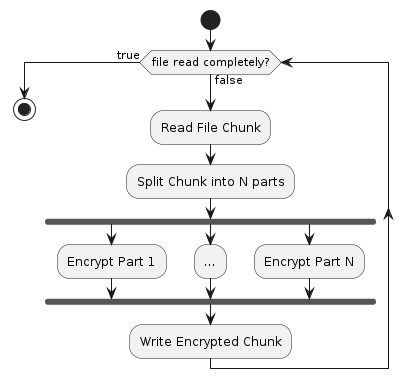
\includegraphics[width=0.5\textwidth]{resources/aes/activity_diagram.png}
    \caption{Diagrama de actividad que representa la paralelización de tareas en AES}
    \label{fig:aes:activity}
\end{figure}

\subsubsection{Rust}

Seleccionamos este lenguaje por su hincapié en la concurrencia \cite{rust:ex:fearless_concurrency} y el rendimiento \cite{com:rust}, propiedades clave para este caso de uso.

La paralelización de tareas se realizó con la biblioteca Rayon \cite{aes:rayon}, muy utilizada por su capacidad para agregar paralelismo en código preexistente, de manera sencilla y segura (es decir, evitando condiciones de carrera).

Como el algoritmo secuencial estaba implementado de manera funcional (utilizando \lstinline{map} para encriptar y desencriptar los bloques), la modificación del código para soportar \english{multithreading} fue muy sencilla. Se puede observar en las figuras \ref{code:rust:aes_sequential} y \ref{code:rust:aes_concurrent} las diferencias entre la implementación secuencial y concurrente del algoritmo de cifrado.

\begin{listing}[h]
\begin{minted}[bgcolor=bg, breaklines]{rust}
let ciphered_blocks = blocks
                      .iter()
                      .map(|block|
                            cipher.cipher_block(*block)).collect::<Vec<_>>();
\end{minted}
\caption{Encriptación secuencial de los bloques en Rust}
\label{code:rust:aes_sequential}
\end{listing}

\begin{listing}[h]
\begin{minted}[bgcolor=bg, breaklines]{rust}
let ciphered_blocks = blocks
                      .par_iter()
                      .map(|block|
                            cipher.cipher_block(block)).collect::<Vec<_>>();
\end{minted}
\caption{Encriptación concurrente de los bloques en Rust}
\label{code:rust:aes_concurrent}
\end{listing}

No fue necesario utilizar ningún mecanismo propio de sincronización, ya que la biblioteca se encarga de distribuir las tareas entre los hilos, recolectarlas y devolverlas en orden.

Por otro lado, la implementación del cifrado y descifrado de bloques se realizó en un \lstinline{struct} llamado \lstinline{AESBlockCipher}, como se ve en el Código~\ref{code:aes:rust_cipher_block} (se omitió el código de descifrado por ser muy similar al de cifrado). La sintaxis se asemeja bastante a la de un lenguaje orientado a objetos, como Java o Python. Sin embargo, las capacidades de Rust en dicho paradigma son muy diferentes \cite{aes:rust_oop}.

\begin{listing}[h]
\begin{minted}[bgcolor=bg, breaklines]{rust}
impl AESBlockCipher {
    pub fn new(cipher_key: [u8; 4 * N_B]) -> Self {
        let expanded_key = AESKey::new_direct(cipher_key);
        let inv_expanded_key = AESKey::new_inverse(cipher_key);
        Self {
            expanded_key,
            inv_expanded_key,
        }
    }
    pub fn cipher_block(&self, data_in: &[u8; 4 * N_B]) -> [u8; 4 * N_B] {
        let mut data_out = [0; 4 * N_B];
        let mut state = State::new_from_data_in(data_in);
        state.add_round_key(&self.expanded_key.data[0..N_B]
                            .try_into()
                            .unwrap());
        for round in 1..N_R {
            state.sub_bytes();
            state.shift_rows();
            state.mix_columns();
            state.add_round_key(
                &self.expanded_key.data[(round * N_B)..((round + 1) * N_B)]
                    .try_into()
                    .unwrap(),
            );
        }
        state.sub_bytes();
        state.shift_rows();
        state.add_round_key(
            &self.expanded_key.data[(N_R * N_B)..((N_R + 1) * N_B)]
                .try_into()
                .unwrap(),
        );
        state.set_data_out(&mut data_out);
        data_out
    }
}
\end{minted}
\caption{Implementación del cifrado de bloques en Rust}
\label{code:aes:rust_cipher_block}
\end{listing}

\subsubsection{Go}

Seleccionamos este lenguaje por su hincapié en la concurrencia \cite{go:ex:concurrency_patterns} y la simplicidad \cite{go:ex:simple}, lo que lo convierte en un buen punto de comparación contra otros lenguajes.

Se utilizaron herramientas nativas de Go para la concurrencia: \lstinline{gorrutinas} \footnote{Las \lstinline{gorutinas} son una abstracción comparable a los hilos} y \lstinline{canales}, en conjunto con el módulo \lstinline{sync} para sincronizar.

En la filosofía del lenguaje prima la idea de \technical{No comunicar compartiendo memoria, sino que, compartir memoria comunicando} \cite{go:ex:sharing}. Por lo cual, esta implementación difiere de las otras, manteniendo un flujo de mensajes continuo, en vez de trabajar sobre un \english{chunk} de memoria compartida.

Se implementó un diseño de tipo \english{pipeline} con una fuente que envía mensajes de trabajo a un conjunto de trabajadores mediante un canal, y un sumidero que los recibe y reordena. En la Figura~\ref{fig:go:robustness} se puede apreciar el despliegue de las gorutinas.

\begin{figure}[h]
    \centering
    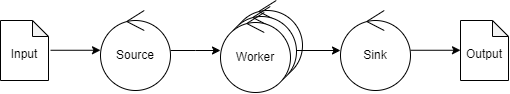
\includegraphics[scale=0.7]{resources/aes/go_robustness.png}
    \caption{Diagrama de robustez que representa las gorutinas de Go en AES}
    \label{fig:go:robustness}
\end{figure}

Podemos ver en el Código~\ref{code:go:process_file} la definición del \english{pipeline}, donde se crean los trabajadores y el sumidero. Estos se comunican mediante canales y se sincronizan mediante \lstinline{waitGroups}. Además, podemos observar que el proceso coordinador actúa también como fuente, enviando los mensajes al canal de ingreso.

\begin{listing}[h]
\begin{minted}[bgcolor=bg, breaklines]{go}
func processFile(inputFile string, outputFile string,
                 key string, numWorkers int) {
    workers_wg := sync.WaitGroup{}
    inputChan := make(chan Message, numWorkers*2)
    sink_wg := sync.WaitGroup{}
    outputChan := make(chan Message, numWorkers*10)

    makeWorkers(numWorkers, &workers_wg, inputChan, outputChan, key)
    MakeSink(&sink_wg, outputChan, outputFile)

    SendMessages(inputFile, inputChan)

    close(inputChan)
    workers_wg.Wait()
    close(outputChan)
    sink_wg.Wait()
}
\end{minted}
\caption{Definición de la función \lstinline{processFile} en Go, que crea los trabajadores y el sumidero (\english{sink}), y envía los bloques a los trabajadores}
\label{code:go:process_file}
\end{listing}

En el código \ref{code:go:cipher_workers} podemos ver la instanciación de los trabajadores de cifrado utilizando la palabra clave \lstinline{go}.

\begin{listing}[h]
\begin{minted}[bgcolor=bg, breaklines]{go}
func MakeCipherWorkers(num int, wg *sync.WaitGroup, plainChan chan Message, cipherChan chan Message, key string) {
	for i := 0; i < num; i++ {
		wg.Add(1)
		go cipherBytes(wg, plainChan, cipherChan,key)
	}
}
\end{minted}
\caption{Definición de la función \lstinline{cipherBytes} en Go, que cifra un conjunto de bloques recibidos a través de un \lstinline{channel}}
\label{code:go:cipher_workers}
\end{listing}

Viendo el comportamiento de los trabajadores de cifrado, detallado en el Código~\ref{code:go:cipher_bytes}, es posible entender mejor el flujo del programa y los mecanismos de sincronización:

\begin{listing}[h]
\begin{minted}[bgcolor=bg, breaklines]{go}
func cipherBytes(wg *sync.WaitGroup, plainChan chan Message,
                 cipherChan chan Message, key string) {	
    cipher, _ := aes.FromString(key)

    for message := range plainChan {
        for i, block := range message.Batch {
            message.Batch[i] = cipher.CipherBlock(block)
        }
        cipherChan <- message
    }

    wg.Done()
}
\end{minted}
\caption{Definición de la función \lstinline{cipherBytes} en Go, que cifra un conjunto de bloques recibidos a través de un \lstinline{channel}}
\label{code:go:cipher_bytes}
\end{listing}

\begin{itemize}
    \item Un proceso leerá \english{batches} de bloques del archivo de entrada y los enviará a los trabajadores mediante un canal. Al terminar de enviar los mensajes, solicitará cerrar el canal, lo que ocurrirá cuando todos los mensajes hayan sido leídos.
    \item Los procesos trabajadores tomarán estos mensajes, encriptarán los bloques y enviarán el mensaje al sumidero.
    \item El sumidero reordenará los mensajes y los escribirá en el archivo de salida.
\end{itemize}

\subsubsection{Julia}

Seleccionamos este lenguaje porque está diseñado para cómputo paralelo \cite{jl:ex:parallelism}, lo que lo convierte en una buena opción para operaciones criptográficas paralelas.

En Julia no se hizo uso de ninguna biblioteca externa, por lo que el desarrollo fue completamente realizado con la biblioteca estándar. Para el \textit{multithreading}, se utilizaron los \textit{threads} de Julia, específicamente las macros \lstinline{@sync} y \lstinline{@spawn}, que fueron un poco más eficientes que \lstinline{@Threads}. En los códigos \ref{code:julia:aes_sequential} y \ref{code:julia:aes_concurrent} es posible visualizar las diferencias entre las implementaciones secuencial y concurrente, respectivamente.

\begin{listing}[h]
\begin{minted}[bgcolor=bg, breaklines]{julia}
function cipher_blocks!(blocks::Vector{Vector{Vector{UInt8}}},
                        buffers_filled::Int,
                        chunks_filled::Vector{Int},
                        expanded_key::AESKey)

    for i in 1:buffers_filled
        aes_block_cipher.cipher_blocks(blocks[i][1:chunks_filled[i]],
                                            expanded_key, chunks_filled[i])
    end
end
\end{minted}
\caption{Encriptación secuencial de los bloques en Julia}
\label{code:julia:aes_sequential}
\end{listing}

\begin{listing}[h]
\begin{minted}[bgcolor=bg, breaklines]{julia}
function cipher_blocks!(blocks::Vector{Vector{Vector{UInt8}}},
                        buffers_filled::Int,
                        chunks_filled::Vector{Int},
                        expanded_key::AESKey)

    @sync for i in 1:buffers_filled
        @spawn aes_block_cipher.cipher_blocks(blocks[i][1:chunks_filled[i]],
                                            expanded_key, chunks_filled[i])
    end
end
\end{minted}
\caption{Encriptación concurrente de los bloques en Julia}
\label{code:julia:aes_concurrent}
\end{listing}

La estructura general de la aplicación es similar a la del resto de los lenguajes, en donde hay una porción sincrónica del programa que lee el archivo a encriptar en un buffer, y luego se divide entre los \textit{threads} para que realicen la tarea de encriptación. Finalmente, se juntan los resultados y se escriben, de manera sincrónica, en un archivo. El mismo proceso se da para la desencriptación, pero en sentido inverso. El buffer tiene un tamaño limitado, por lo que este proceso se itera hasta haber encriptado o desencriptado todo el archivo.

La estructura general de la aplicación es similar a la del resto de lenguajes, en donde hay una porción sincrónica del programa que lee el archivo a encriptar en un buffer, y luego se divide entre los \english{threads} para que realicen la tarea de encriptación, para finalmente juntar los resultados y escribirlo, de manera sincrónica, a un archivo. El mismo proceso se da para la desencriptación, pero en sentido inverso. El buffer tiene un tamaño limitado, por lo que se itera este proceso hasta haber encriptado o desencriptado todo el archivo.

Un detalle notable es que se pudo usar las matrices que provee el lenguaje, a diferencia de otros casos que tuvieron que implementar sus propias matrices usando vectores o arreglos. Estas matrices fueron muy útiles ya que tenían implementadas operaciones que necesitábamos. Por ejemplo, la función \lstinline{mix_columns!} (definida en el estándar como \lstinline{MixColumns}) utiliza la macro \lstinline{@view} y la sintaxis de matrices para obtener fácilmente la columna i-ésima del estado, como se observa en la Figura~\ref{code:julia:aes_mix_columns}. Sin embargo, algunas de estas tuvieron que ser reescritas en pos de mejorar la \english{performance}.

\begin{listing}[h]
\begin{minted}[bgcolor=bg, breaklines]{julia}
function mix_columns!(_state::State)
    for i in 1:N_B
        @inbounds col = @view _state[:, i]
        mix_column!(col)
    end
end
\end{minted}
\caption{Implementación de la función \lstinline{mix_columns!} en Julia}
\label{code:julia:aes_mix_columns}
\end{listing}

\subsubsection{Scala}

Seleccionamos este lenguaje porque posee amplios recursos para aplicaciones concurrentes, gracias a su interoperabilidad con las bibliotecas de Java \cite{scala:ex:why_scala_3}.

Al igual que los lenguajes anteriores, la implementación se divide en dos etapas:

\begin{itemize}
    \item Lectura y escritura por partes (\english{chunks}) de los archivos de prueba, utilizando bibliotecas estándar de Java para garantizar el \english{buffering} de entrada y salida.
    \item Utilización de un modelo \english{fork-join} para el cifrado y descifrado de los bloques. La idea subyace en tener un conjunto de $N$ hilos trabajadores que se encargarán del cifrado o descifrado de los bloques, mientras que el hilo principal será quien los junte para obtener la estructura original.
\end{itemize}

En las figuras \ref{code:scala:aes_sequential} y \ref{code:scala:aes_concurrent} se pueden observar las versiones secuencial y concurrente del algoritmo, respectivamente, según el modelo comentado. Notar que la única diferencia significativa es el agregado de los métodos \lstinline{par} y \lstinline{toVector}.

\begin{listing}[h]
\begin{minted}[bgcolor=bg, breaklines]{scala}
def applyOperationsAndCompare(cipher: AESCipher,
                              blocks: Vector[Array[Byte]]): Boolean = {
    val cipheredBlocks = blocks
                         .map(block => cipher.cipherBlock(block))
    val decipheredBlocks = cipheredBlocks
                           .map(block => cipher.invCipherBlock(block))
}
\end{minted}
\caption{Encriptación y desencriptación secuencial en Scala}
\label{code:scala:aes_sequential}
\end{listing}


\begin{listing}[h]
\begin{minted}[bgcolor=bg, breaklines]{scala}
def applyOperationsAndCompare(cipher: AESCipher,
                              blocks: Vector[Array[Byte]]): Boolean = {
    val cipheredBlocks = blocks
                         .par.map(block => cipher.cipherBlock(block)).toVector
    val decipheredBlocks = cipheredBlocks
                           .par.map(block => cipher.invCipherBlock(block)).toVector
}
\end{minted}
\caption{Encriptación y desencriptación concurrente en Scala}
\label{code:scala:aes_concurrent}
\end{listing}

Ell cifrado y descifrado de bloques se implementó en una clase llamada \lstinline{AESBlockCipher}, como se ve en el Código~\ref{code:scala:aes_cipher_block}.

\begin{listing}[h]
\begin{minted}[bgcolor=bg, breaklines]{scala}
class AesBlockCipher(val expandedKey: AESKey, val invExpandedKey: AESKey) {

  def cipherBlock(dataIn: Array[Byte]): Array[Byte] = {
    val dataOut = new Array[Byte](4 * Constants.N_B)

    val state = new State(dataIn)

    state.addRoundKey(expandedKey.data.slice(0, Constants.N_B))

    for (round <- 1 until Constants.N_R) {
      state.subBytes()
      state.shiftRows()
      state.mixColumns()
      state.addRoundKey(expandedKey.data.slice(round * Constants.N_B, (round + 1) * Constants.N_B))
    }

    state.subBytes()
    state.shiftRows()
    state.addRoundKey(expandedKey.data.slice(Constants.N_R * Constants.N_B, (Constants.N_R + 1) * Constants.N_B))

    state.setDataOut(dataOut)

    dataOut
  }
}
\end{minted}
\caption{Implementación del cifrado de bloques en Scala}
\label{code:scala:aes_cipher_block}
\end{listing}

\subsubsection{Zig}

Seleccionamos este lenguaje por ser una alternativa innovadora y con hincapié en la \english{performance} \cite{zig:ex:zig_in_100_sec}.

Como se trata de un lenguaje bastante nuevo, no existen muchas bibliotecas relacionadas con la concurrencia. Por lo tanto, la paralelización de tareas se realizó con la primitiva \lstinline{std.Thread.spawn}, que funciona de manera similar a la función \lstinline{pthread_create} de C. Se aplicó la técnica de \english{Work Stealing} para la distribución de tareas, utilizando una implementación propia de una \english{Queue} \english{thread-safe}. Los hilos trabajadores realizan la encriptación/desencriptación y guardan el resultado en la dirección de memoria indicada. El código resultante fue un \lstinline{struct} llamado \lstinline{ParallelMap}, que imita la funcionalidad de las implementaciones en Rust y Scala.

En el Código~\ref{code:zig_parallel_map} se puede observar, entre otras cosas, la forma en que Zig implementa los \english{generics}. Se define una función que recibe valores de tipo \lstinline{type}, y devuelve un nuevo tipo. Los \english{generics} \lstinline{R} y \lstinline{S} corresponden a los tipos de entrada y salida del \lstinline{map}, respectivamente, y \lstinline{Ctx} es un argumento adicional que puede recibir la función que mapea los valores. En nuestro caso de uso, \lstinline{R} y \lstinline{S} corresponden a bloques de 128 bits, y \lstinline{Ctx} es el cifrador de bloques AES. 

Es interesante notar que el parámetro \lstinline{Ctx} se requiere debido a que las funciones anónimas no pueden capturar variables del entorno. Nuestro caso de uso requiere, como mínimo, el valor de la clave utilizada para encriptar/desencriptar.

\begin{listing}[h]
\begin{minted}[bgcolor=bg, breaklines]{zig}
pub fn ParallelMap(comptime R: type,
                   comptime S: type,
                   comptime Ctx: type) type {
    return struct {
        pub const Self = @This();
        allocator: std.mem.Allocator;

        pub fn init(config: Config) !Self

        pub fn destroy(self: *Self) !void

        pub fn map(self: *Self,
                   ctx: *const Ctx,
                   func: *const fn(*const Ctx, R) S,
                   input: []const R,
                   results: []S) !void
    };
}
\end{minted}
\caption{Definición abreviada del \lstinline{ParallelMap} en Zig}
\label{code:zig_parallel_map}
\end{listing}

En el Código~\ref{code:zig_queue} se muestra un ejemplo de utilización de los \english{allocators}, que permiten definir de manera precisa cómo se reserva la memoria. La elección de un \english{allocator} puede modificar en gran medida el rendimiento del código. El \english{allocator} más básico, \lstinline{std.heap.page_allocator}, realiza una \english{syscall} por cada llamada a \lstinline{create}, mientras que un \lstinline{std.heap.FixedBufferAllocator} no realiza ninguna, sino que utiliza un \english{buffer} predefinido.

\begin{listing}[h]
\begin{minted}[bgcolor=bg, breaklines]{zig}
pub fn push(self: *Self, value: T) !void {
    var new_node = try self.allocator.create(TailQueueType.Node);
    new_node.data = value;

    self.lock.lock();
    self.unsafe_queue.append(new_node);
    self.lock.unlock();

    self.not_empty().post();
}
\end{minted}
\caption{Implementación del método \lstinline{push} de la \english{Queue} \english{thread-safe} en Zig}
\label{code:zig_queue}
\end{listing}

\newpage

\subsection{Métricas}

A continuación se realiza un análisis de las métricas tomadas. En el anexo en la sección~\ref{sec:anex:metrics:aes} (\hyperref[sec:anex:metrics:aes]{\nameref*{sec:anex:metrics}: \nameref*{sec:anex:metrics:aes}}) se incluyen algunos datos adicionales.

\subsubsection{Despliegue}

En el Cuadro~\ref{tab:aes:metrics} se pueden observar los resultados obtenidos. El significado de cada una de las métricas es el siguiente:

\begin{itemize}
    \item \textbf{Duración}: tiempo que tardó el programa en ejecutarse.
    \item \textbf{Uso de memoria}: uso de memoria promedio del \english{container} que ejecuta el programa.
    \item \textbf{Uso de CPU}: uso de CPU promedio del \english{container} que ejecuta el programa.
\end{itemize}

Los valores del cuadro son relativos, al igual que las métricas del área anterior (sección~\ref{sec:gs_metrics}).

\begin{table}[h]
\centering
\begin{tabular}{|l|c|c|c|c|c|}
\hline
\multicolumn{1}{|c|}{Métrica} & Rust & Go & Julia & Scala & Zig \\ \hline
Duración & $100.00\%$& $603.55\%$& $94.08\%$& $\numprint{1491.12}\%$& $143.79\%$\\ \hline
Uso de memoria & $100.00\%$& $6.88\%$& $237.23\%$& $245.02\%$& $0.98\%$\\ \hline
Uso de CPU & $100.00\%$& $112.33\%$& $76.33\%$& $59.67\%$& $77.33\%$\\ \hline
\end{tabular}
\caption{Métricas de Criptografía. Basado en mediciones en FaMAF-2, relativas a Rust  (Ver Cuadro~\ref{tab:aes:famaf_2})}
\label{tab:aes:metrics}
\end{table}

% FIXME!!!: Completar
De estos datos, es posible obtener algunas conclusiones preliminares:

\begin{itemize}
    \item El tiempo que tarda Scala en ejecutarse es mucho mayor que el del resto: esto era esperable, pues se trata del único lenguaje que no compila a código nativo.
    \item Go y Zig utilizaron una cantidad de memoria comparable: esto es muy interesante, pues ambos lenguajes ofrecen mecanismos de manejo de memoria muy diferentes: Go utiliza un recolector de basura, mientras que en Zig se debe reservar y liberar manualmente.
\end{itemize}

\subsubsection{Generales}

Se evaluaron, al igual que en el área de Sistemas Distribuidos, métricas relacionadas al tiempo de desarrollo y espacio de las imágenes de Docker utilizadas (ver la Sección~\ref{sec:general_metrics} para una descripción detallada de las mismas). Los resultados se pueden observar en el Cuadro~\ref{tab:aes:relative_general_metrics}.

\begin{table}[h]
\centering
\begin{tabular}{|l|c|c|c|c|c|}
\hline
\multicolumn{1}{|c|}{Métrica} & Rust & Go & Julia & Scala & Zig \\ \hline
Tiempo & 125\% & 75\% & 150\% & 75\% & 125\% \\ \hline
Espacio & x$0.56$ & x$1.45$ & x$91.9$ & x$24.6$ & x$1.50$ \\ \hline
\end{tabular}
\caption{Métricas generales correspondientes al área de Criptografía}
\label{tab:aes:relative_general_metrics}
\end{table}

\subsection{Experiencias}

Se realizó una evaluación subjetiva de los lenguajes de programación según nuestra experiencia desarrollando con ellos.

\subsubsection{Comparación}

Los atributos que se tuvieron en cuenta a la hora de realizar la comparación entre lenguajes coinciden con los del caso de uso anterior (ver la Sección~\ref{sec:subjective_comparison} para una descripción de los mismos).
Los resultados se expresan en el Cuadro~\ref{tab:aes:experiences}.

\begin{table}[h]
\centering
\begin{tabular}{|l|c|c|c|c|c|}
\hline
\multicolumn{1}{|c|}{Atributo} & Rust & Go & Julia & Scala & Zig \\ \hline
Expresividad & \goodMetric{5} & 3 & \goodMetric{4} & \goodMetric{4} & 3 \\ \hline
Simplicidad & \badMetric{1} & \goodMetric{5} & 3 & \goodMetric{4} & \goodMetric{4} \\ \hline
Memoria & \goodMetric{5} & \goodMetric{4} & 3 & 3 & \goodMetric{5} \\ \hline
Errores & \goodMetric{5} & 3 & 3 & 3 & \badMetric{2} \\ \hline
Concurrencia & \goodMetric{5} & \goodMetric{5} & \goodMetric{5} & \goodMetric{5} & \badMetric{2} \\ \hline
Bibliotecas & \goodMetric{5} & \goodMetric{5} & \goodMetric{4} & \goodMetric{4} & \badMetric{0} \\ \hline
\end{tabular}
\caption{Resumen de la comparación de atributos para el área de Criptografía}
\label{tab:aes:experiences}
\end{table}

\subsubsection{Rust}

La experiencia de desarrollo en general es muy buena, aunque puede resultar difícil de aprender en un principio. Las abstracciones en Rust son \technical{de cero costo}, lo que significa que no perjudican a la \english{performance}.

Rust destaca por sobre el resto de lenguajes introduciendo el concepto de \english{ownership}, que tiene la interesante característica de resolver dos grandes problemas, aparentemente no relacionados

\begin{itemize}
    \item Garantizar la seguridad de la memoria: uno de los inconvenientes que suelen tener los lenguajes de bajo nivel, es el manejo correcto de la memoria. Los \english{memory leaks} pueden generar un constante deterioro en programas que se ejecutan de manera continua, como los servidores, al punto de tener que reiniciarlos. Esto no ocurre en Rust, a menos que se apliquen malas prácticas a propósito (como el uso de \lstinline{std::mem::forget}). Los chequeos de memoria se realizan en tiempo de compilación, por lo que tampoco incurren en un costo de \english{performance}.
    \item Evitar errores de concurrencia: el compilador es capaz de detectar situaciones en las cuales es posible que ocurran errores propios de un programa concurrente.
    
    Un clásico ejemplo es el de una variable contadora compartida por múltiples hilos. La acción de incrementar una variable suele ser una operación que involucra múltiples operaciones no atómicas del procesador: copiar el valor a un registro, actualizarlo y copiarlo nuevamente en la memoria. Si estas operaciones se intercalan, los errores comienzan a surgir rápidamente.
    
    En Rust, un programa con esas características ni siquiera compilaría, forzando al programador a buscar una solución correcta. Para solucionarlo se puede utilizar, por ejemplo, las abstracciones \lstinline{std::sync::Arc} y \lstinline{std::sync::Mutex} para encapsular la variable y compartirla entre múltiples hilos, tal y como se observa en el Código~\ref{code:aes:rust_concurrency}.
\end{itemize}

\begin{listing}[h]
\begin{minted}[bgcolor=bg, breaklines]{rust}
use std::thread;
use std::sync::{Mutex, Arc};

fn main() {
    let counter = Arc::new(Mutex::new(0));
    let mut handles = vec![];

    for _ in 0..10 {
        let counter = Arc::clone(&counter);
        let handle = thread::spawn(move || {
            let mut num = counter.lock().unwrap();
            *num += 1;
        });
        handles.push(handle);
    }
    for handle in handles {
        handle.join().unwrap();
    }
    println!("Result: {}", *counter.lock().unwrap());
}
\end{minted}
\caption{Implementación de un contador multihilo en Rust}
\label{code:aes:rust_concurrency}
\end{listing}

Estas características del lenguaje tienen como desventaja el elevado tiempo de compilación. Esto suele ser un muy buen \english{trade-off} en situaciones donde el rendimiento es crítico, como en este caso de uso, pero puede dificultar el prototipado.

En cuanto al desarrollo particular del algoritmo AES, la biblioteca Rayon simplificó enormemente el paso de código secuencial a código concurrente. En base a esto, se decidió hacer la mayor parte del código basándose en programación funcional, de manera de adaptarse fácilmente a la biblioteca; utilizando iteradores y operaciones de \lstinline{map}, \lstinline{reduce}, etc.

Por otro lado, el uso de los \lstinline{structs} de \lstinline{BufReader} y \lstinline{BufWriter}, que pertenecen a la biblioteca estándar, mejoró mucho la \english{performance}, ya que las lecturas y escrituras a disco eran el cuello de botella. Se llegó a esta conclusión corriendo el programa con ambas configuraciones y comparando el tiempo de encriptación y desencriptación de cada bloque.

\subsubsection{Go}


La implementación de la lógica de negocio se realizó en base a la implementación en Rust. El proceso fue extremadamente simple y directo, presentando mínimos inconvenientes. La velocidad de desarrollo fue notable al tener la lógica definida, tomando mucho menos tiempo del esperado.

No se encontró una biblioteca convincente para iteración paralela. Por lo tanto, se optó por implementar un mecanismo propio utilizando el patrón \textit{pipeline}. Este patrón fue elegido inicialmente en base a la filosofía del lenguaje \cite{go:ex:sharing} e influenciado por el desarrollo del \nameref{sec:sis_dist}. Esta elección se vio reforzada posteriormente, dado que este patrón de concurrencia es comúnmente utilizado en Go \cite{go:ex:pipelines}.

Dado que la entrada es por archivo y de longitud indefinida, se implementó un \textit{pipeline} adaptado a procesamiento continuo. El desarrollo de este fue simple y directo. Go proporciona todas las herramientas necesarias para su desarrollo y demuestra estar preparado para la aplicación de mecanismos concurrentes.

El uso de \textit{gorutinas} y canales simplifica la repartición de tareas, mientras que la sincronización de cierre se maneja con el cierre de los canales y el uso de \lstinline{WaitGroups}.

Como consecuencia del modelo de procesamiento, las tareas pueden llegar desordenadas al sumidero. Sin embargo, el caso de uso requiere la escritura de bloques ordenados, por lo que se implementó un mecanismo de reordenamiento en el sumidero utilizando un \english{heap}.

El paquete \lstinline{buffio} de la biblioteca estándar ofrece un buen soporte nativo para la lectura y escritura segura y optimizada (mediante \english{buffers}) de archivos y \english{streams} en general. Esto simplificó el desarrollo al mismo tiempo que mejoró la \english{performance}.

\subsubsection{Julia}

En Julia, al igual que el resto de lenguajes, lo primero que se desarrolló fue el cifrado y descifrado de un único bloque. Como esta parte del código solo utiliza estructuras de tamaño fijo, se intentó utilizar la biblioteca \lstinline{StaticArrays.jl} \cite{jl:lib:staticarrays}, pues su documentación sugería que su uso podría conllevar una mejora de rendimiento. Sin embargo, nos encontramos con varios problemas al intentar trabajar con esta biblioteca, por lo que decidimos utilizar los vectores que provee la biblioteca estándar.

A pesar de este contratiempo, el desarrollo del algoritmo arrojó buenos resultados. Al realizar pruebas individuales, los resultados fueron prometedores, aunque el elevado uso de memoria despertó ciertas preocupaciones.

Durante el desarrollo del algoritmo surgieron otros problemas menores. Por ejemplo, Julia utiliza índices que comienzan en 1 y rangos cerrados, debido a que sus orígenes se remontan a la comunidad matemática. Como el resto de las implementaciones utilizan rangos semi-abiertos comenzados en 0, esto causó errores al adaptar el algoritmo. Si bien no fueron problemas graves, requirieron precauciones adicionales para evitar errores difíciles de detectar si el desarrollador no está familiarizado con estas diferencias. Otro desafío común fueron los mensajes de error, que a menudo no indicaban correctamente la ubicación del error en el código, lo que prolongó el tiempo necesario para el \english{debugging}.

Después de implementar y verificar el funcionamiento correcto del algoritmo, procedimos a integrarlo con paralelismo. En Julia, el paralelismo es muy simple y directo. Como se muestra en el Código~\ref{code:aes:julia_multithreading}, tomado de ENCCS \cite{jl:ex:encss_jl_threading}, paralelizar código en Julia es tan sencillo como agregar la macro \lstinline{@threads} antes de un bucle \lstinline{for}. Julia maneja automáticamente la ejecución de la rutina y el acceso a la memoria compartida.


\begin{listing}[h]
\begin{minted}[bgcolor=bg, breaklines]{julia}
using Base.Threads

function threaded_sqrt_array(A)
    B = similar(A)
    @threads for i in eachindex(A)
        @inbounds B[i] = sqrt(A[i])
    end
    B
end
\end{minted}
\caption{Ejemplo de utilización de las macros \lstinline{@threads} y \lstinline{@inbounds}}
\label{code:aes:julia_multithreading}
\end{listing}

Con estas consideraciones, pensamos que paralelizar el código sería una tarea sumamente fácil, implicando simplemente agregar una línea de código. Sin embargo, al medir el desempeño de nuestro algoritmo con múltiples hilos, descubrimos que el rendimiento era peor que la versión sincrónica. Esta situación nos llevó a investigar las causas de tal pérdida de rendimiento. Durante esta exploración, descubrimos varias herramientas que Julia ofrece para mejorar la \english{performance}, a saber:

\begin{itemize}
    \item \lstinline{@inbounds}: sirve para indicarle al intérprete que no realice la verificación de límites cuando se accede a un vector. Esto es muy útil para algoritmos criptográficos que siempre operan sobre dimensiones definidas.
    \item Soporte para operaciones SIMD\footnote{SIMD: acrónimo de \english{Single Instruction, Multiple Data} (``una instrucción, múltiples datos'')}: autoriza al intérprete para reordenar la ejecución de un ciclo de la manera más beneficiosa para el programa. Es importante asegurar que las operaciones en ese ciclo sean independientes para evitar introducir errores.
    \item \lstinline{@view}: permite crear una referencia a un arreglo, en lugar de una copia. Esto permitió disminuir significativamente el número de veces que se reserva memoria.
    \item Funciones terminadas con `!': en Julia, una función que termina con `!' indica que modifica sus argumentos de entrada. En muchos casos, las funciones de la biblioteca estándar tienen una versión con `!' y otra sin. Usualmente la versión con `!' es más eficiente, ya que realiza la operación en el lugar, reduciendo la necesidad de reservar memoria adicional.
\end{itemize}

Al hacer uso de todas estas herramientas, la eficiencia del código mejoró enormemente. No obstante, la versión con un solo hilo seguía siendo más rápida que la versión multihilo. Esto nos llevó a pensar que la falta de rendimiento utilizando paralelismo se debía a un caso de \english{false sharing}\footnote{False sharing: mecanismo por el cual el protocolo de caché puede forzar a un programa a recargar todo un bloque de caché a pesar de no existir necesidad para ello, debido a que se intenta acceder periódicamente a datos que nunca serán alterados pero que comparten bloques de caché con datos que sí son alterados.}. En nuestro programa, para leer el archivo que se quería encriptar, se leía sobre un \english{buffer} que luego se dividía en diferentes partes, las cuales eran pasadas a distintas hilos para su encriptación. Julia no nos brinda control directo sobre cómo se reserva la memoria de la aplicación ni sobre cómo se controla el acceso entre diferentes hilos. Esta característica del lenguaje puede considerarse una ventaja, pues simplifica su uso, pero la pérdida de rendimiento la convierte en un problema. Un método recomendado para evitar el \english{false sharing} es espaciar los \english{buffers} de cada hilo en relación a dónde se ubican en la memoria. Como no hay una forma explícita de hacer esto en Julia, recurrimos a probarlo reservando \english{buffers} vacíos entre los verdaderos \english{buffers} que se iban a usar para el algoritmo. Luego de hacer este \english{refactor}, se probó nuevamente el programa, y no se notó mejoría en el rendimiento, por lo que se concluyó que ese no era el problema.

Nuestro siguiente paso en la búsqueda de una solución fue usar un \english{profiler}, que resultó ser muy agradable de usar. Este \english{profiler} genera un gráfico que permite navegar a través de cada función ejecutada, y las funciones están ordenadas verticalmente, según el \english{stack}; y horizontalmente, según cuánto tiempo estuvieron ejecutándose en relación al tiempo de ejecución total. Además, es posible visualizar el programa en su totalidad o por hilo. Cuando se realizó el primer \english{profile} de la aplicación, los resultados parecían indicar que el 75\% del tiempo no había ninguna función ejecutándose. Luego de un poco de investigación, se descubrió que el \english{profiler} omitía las funciones ejecutadas en C. Sin embargo, este inconveniente pudo ser solucionado cambiando la versión del \english{profiler} y agregando un \english{flag} especial.

La ejecución de este nuevo \english{profiler} permitió detectar que el verdadero problema era el recolector de basura. Como se encuentra escrito en C, no fue posible visualizarlo en la primera ejecución del \english{profiler}. Luego de un período de investigación, se descubrió que el recolector de basura es parcialmente \english{multi-threaded}, y como tal, bloqueaba el sistema al momento de ejecutarse. Esto nos pareció una decisión de diseño cuestionable para un lenguaje que proclama su idoneidad para el procesamiento en paralelo. No obstante, quedó claro que una reducción en el número de invocaciones del recolector de basura traería aparejada una mejoría en el rendimiento del programa. Para conseguir esto, fue de mucha ayuda una macro llamada \lstinline{@time}.

Esta macro no solo indica cuánto tiempo tardó en ejecutarse una función, sino que también indica cuántas reservas de memoria hubo dentro de ella. Gracias a esto, fue posible observar los puntos críticos del sistema y cambiar el diseño de nuestro código, a fin de minimizar las reservas de memoria. Un caso destacable fue el de la función \lstinline{circshift!}, cuyo uso era crítico para el algoritmo ya que se usaba para mezclar las filas de la tabla, uno de los pasos más repetidos. El nombre de la función, al terminar con \lstinline{!}, sugiere que la operación se realiza sobre el argumento de entrada, y por lo tanto no debería reservar memoria. Contrario a nuestra hipótesis, esta función estaba reservando memoria cada vez que se ejecutaba, bloqueando el resto del programa en el proceso. Para resolver esto, fue necesario reescribir la función.

Luego de todas estas optimizaciones, el esfuerzo rindió frutos y Julia logró el mejor rendimiento de todos los lenguajes explorados. Claramente, para esto se requirió un trabajo y conocimiento mayor, lo que sin duda debería considerarse al momento de elegir un lenguaje para implementar un programa de estas características.

\subsubsection{Scala}

Scala no tiene la capacidad de diferencia entre los distintos tipos de enteros (signados, no signados o aquellos con diferente cantidad de bits/bytes). En este caso, tenemos los tipos \lstinline{int} (tipo nativo) e \lstinline{Integer} (clase de Java) que son los mismos dos tipos/clases con los que nos podemos encontrar en Java. Sin embargo, sí existe el tipo de dato ``Byte`` que nos permitió hacer una transferencia/paralelismo uno a uno con la especificación del estándar de AES. Al mismo tiempo, el lenguaje presentó una expresividad muy alta debido a que permite un híbrido entre programación orientada a objetos y programación funcional.Esto hace que el código sea más legible y mantenible, algo que puede ser muy interesante en proyectos grandes, como una alternativa a Java. Además, el hecho de ser híbrido permite programar puramente en POO (si se viene del ámbito de C\#, Java o incluso C++) o programar puramente en estilo funcional.

En cuanto al uso de bibliotecas, Scala no tiene una biblioteca que nos provea de un cliente nativo para enviar datos a Graphite, por lo que optamos por utilizar una biblioteca de Java (mantenida por DataDog).

\subsubsection{Zig}

Es un lenguaje de programación principalmente imperativo. Resultó fácil de aprender, introduciendo algunos conceptos nuevos pero sencillos, como por ejemplo la capacidad de definir números de una cantidad arbitraria de \english{bits}.

El punto más destacado del lenguaje es el manejo de memoria. La solución que ofrece es muy simple: las funciones aceptan \english{allocators}, que son estructuras que permiten reservar y liberar memoria. Lo interesante es que dichas acciones no involucran necesariamente memoria del \english{heap} ni una llamada al sistema (\english{syscall}). El uso de esta abstracción a lo largo de toda la biblioteca estándar es muy beneficioso: en algunas ocasiones, una estructura (por ejemplo, una lista) puede ser lo bastante pequeña como para definirse en el \english{stack}, y otras veces se requiere en el \english{heap}. Gracias a los \english{allocators}, la elección entre uno u otro es tan simple como la modificación de un parámetro de inicialización, tal y como se observa en los códigos \ref{code:aes:zig_fba} y \ref{code:aes:zig_gpa}.

\begin{listing}[h]
\begin{minted}[bgcolor=bg, breaklines]{zig}
const std = @import("std");
const ArrayList = std.ArrayList;

pub fn main() !void {
    var buffer: [1000]u8 = undefined;
    var fba = std.heap.FixedBufferAllocator.init(&buffer);
    const allocator = fba.allocator();
    var list = ArrayList(u32).init(allocator);
    try list.append(1);
    std.debug.print("list[0] = {}\n", .{list.items[0]});
    list.deinit(); // Libera la memoria del buffer estático
}
\end{minted}
\caption{Inicialización de una lista en el \english{stack} por medio de un \lstinline{FixedBufferAllocator}, en Zig}
\label{code:aes:zig_fba}
\end{listing}

\begin{listing}[h]
\begin{minted}[bgcolor=bg, breaklines]{zig}
const std = @import("std");
const ArrayList = std.ArrayList;

pub fn main() !void {
    var gpa = std.heap.GeneralPurposeAllocator(.{}){};
    const allocator = gpa.allocator();
    var list = ArrayList(u32).init(allocator);
    try list.append(1);
    std.debug.print("list[0] = {}\n", .{list.items[0]});
    list.deinit(); // Libera la memoria del heap
}
\end{minted}
\caption{Inicialización de una lista en el \english{heap} por medio de un \lstinline{GeneralPurposeAllocator}, en Zig}
\label{code:aes:zig_gpa}
\end{listing}

Algunos de los \english{allocators} más usados son:

\begin{itemize}
    \item \english{Page allocator}: es el más básico de todos, pues realiza una \english{syscall} cada vez que se reserva o libera memoria.
    \item \english{Arena allocator}: simplifica la liberación de toda la memoria reservada a un único \english{free}.
    \item \english{Fixed buffer allocator}: permite reservar memoria a partir de un \english{buffer} predefinido, que a su vez puede encontrarse en el \english{heap} o en el \english{stack}.
    \item \english{General purpose allocator}: implementación centrada en la seguridad, que previene errores de tipo \english{double-free}, \english{use-after-free} y \english{memory leaks}. También es \english{thread-safe}.
    \item \english{C allocator}: muy rápido, pero con muy pocas \english{features} de seguridad.
\end{itemize}

Cabe destacar que es posible definir nuevos \english{allocators} con un comportamiento diferente.

% FIXME: ver comentario

Por otro lado, el lenguaje tiene carencias en otras áreas. El manejo de errores es pobre, por lo que nos resultó dificultoso realizar \english{debugging}. Algunos errores no son descriptivos o indican líneas incorrectas debido a que el propio compilador presenta errores. Además, como en la mayoría de los lenguajes, no está permitido compilar si hay errores, pero Zig presenta errores que deberían ser \english{warnings} (por ejemplo variables o parámetros sin utilizar, que suele suceder cuando estamos en proceso de desarrollo). 

Uno de nuestros objetivos era probar el modelo de concurrencia nativo del lenguaje y eso no fue posible puesto que las funcionalidades asincrónicas fueron removidas a partir de la v0.11 (se encontraba en v0.12 a la fecha del desarrollo) porque generaban errores. Esta inestabilidad genera que no se encuentran bibliotecas útiles a raíz de que se introducen \english{breaking changes} entre versiones y el código queda rápidamente obsoleto. Al ser lenguaje que se encuentra en las primeras fases de su desarrollo, posee una mala integración con los entornos de desarrollo; y suelen renombrar funciones o métodos que son comunes para la industria. Por ejemplo, al utilizar semáforos, la operación \english{signal} es llamada \english{post}. Si bien es un inconveniente menor, dificulta innecesariamente el proceso de aprendizaje e investigación de la biblioteca estándar.

Este tipo de errores o falencias entorpecen el desarrollo, pero el equipo de Zig está trabajando activamente en solucionarlos. Cabe destacar que el lenguaje aún no ha alcanzado su primera versión estable.

Al mismo tiempo, hay algunas características complementarias interesantes:
\begin{itemize}
    \item Posee un caché para acelerar la compilación y la ejecución de los tests (si no hay cambios en el código, los tests no se ejecutan de nuevo).
    \item El proceso de compilación hace chequeos robustos.
    \item Se puede especificar la evaluación en tiempo de compilación.
    \item La comunidad es descentralizada.
    \item Tiene un mecanismo para traducir código de C a Zig: si bien no se utilizó para la realización de este trabajo, la documentación indica que es capaz de traducir satisfactoriamente la mayor parte del código de C \cite{aes:zig:translate_c}.
\end{itemize}

La experiencia deja que desear, pero no descartamos que a futuro pueda posicionarse como un lenguaje competitivo.

\subsection{Conclusiones}

A continuación se presentan nuestras conclusiones, organizadas por lenguaje, en orden de preferencia para este caso de uso.

\subsubsection{Rust}

El rendimiento es muy bueno y el lenguaje provee herramientas que permiten generar código óptimo. El manejo de memoria destaca particularmente, siendo potente y directo (si bien un tanto complejo). Los conceptos de \english{ownership} y \english{lifetimes} posibilitan la liberación de memoria cuando ya no es necesaria, lo cual resulta una alternativa atractiva frente a un recolector de basura. Su buen rendimiento también se debe a sus `abstracciones de cero costo' que se resuelven en tiempo de compilación.

La experiencia de desarrollo es buena. No es un lenguaje simple, pero dado que el equipo de trabajo ya tenía cierta experiencia con el lenguaje, no sufrió las dificultades que se encuentran al usarlo por primera vez. Posee buenas herramientas que facilitan el desarrollo, entre las que destacan el compilador, pues brinda errores muy descriptivos e incluso provee sugerencias para su resolución; y bibliotecas como Rayon, que simplifican el paralelismo.

Es uno de los lenguajes más complejos dentro de los evaluados, pero siendo que el caso de uso amerita cierta complejidad, no lo consideramos una carencia.

Como observamos buen rendimiento y buena experiencia de desarrollo, y siendo que permite un manejo de memoria suficientemente detallado, lo consideramos el lenguaje óptimo para el este dominio de aplicación.

\subsubsection{Julia}

El rendimiento es muy bueno, siendo las optimizaciones necesarias y trabajosas. Provee varias herramientas interesantes para optimizar el código, tales como las macros \lstinline{@inbounds}, \lstinline{@view} y \lstinline{@time}.

Es uno de los lenguajes más complejos dentro de los evaluados, pero siendo que el caso de uso amerita cierta complejidad, no lo consideramos una carencia.

Si bien el rendimiento es bueno y la experiencia de desarrollo también lo es en general, la implementación parcial \english{multi-threaded} del recolector de basura es un inconveniente clave. Objetos hasta 2kB son asignados en un thread disponible de una pool de asignaciones, mientras que objetos mayores a 2kB son asignados dinámicamente en el \english{heap}. A raíz de esto, es posible optimizar el código a modo de minimizar su impacto.

\subsubsection{Go}

El rendimiento es comparativamente peor a otros lenguajes. Go no provee muchas herramientas para la optimización a bajo nivel. Por ejemplo: la asignación y liberación de memoria es generalmente muy buena, pero, es completamente automática y no se proveen mecanismos para su control.

El lenguaje basa su diseño en el siguiente principio: \blockquote[\cite{go:ex:effective_concurrency}]{\english{Don't communicate by sharing memory; share memory by communicating}} . Esto implica un \english{trade-off} entre simplicidad y \english{performance} que afecta significativamente a este caso, donde otros lenguajes no incurren en tanto \english{overhead} de comunicación.

La experiencia de desarrollo es muy buena, siendo fácil crear y sincronizar tareas. A pesar de esto, su desempeño hace que no sea una opción apropiada para este caso de uso, salvo que se busque simplicidad en el desarrollo o un prototipo rápido.

\subsubsection{Zig}

El rendimiento es bueno. Las herramientas que provee para gestionar memoria son efectivas.

La experiencia de desarrollo deja que desear. Si bien es fácil de aprender, el desarrollo puede ser complicado debido, principalmente, a la dificultad para realizar debugging, encontrando a veces errores que son incorrectos; y la falta de retrocompatibilidad debida a la introducción de \english{breaking changes} en las versiones sucesivas, lo cual conlleva una falta de bibliotecas compatibles. 

Se tienen expectativas de que mejore mucho a medida que el lenguaje crezca, siendo que aún no está en la versión 1.0. Pero la introducción constante de \english{breaking changes} lo hace un lenguaje poco maduro para su uso comercial.

\subsubsection{Scala}

En comparación con el resto de lenguajes, su rendimiento es muy malo. Desde la falta de tipos sin signo se notó la carencia de herramientas óptimas para este caso de uso.

La experiencia de desarrollo es buena. Cumple su objetivo de crear código mantenible, pero no compite en \english{performance} como para que la buena experiencia de desarrollo lo justifique en este caso.

\newpage

\section{Dominio de aplicación: Redes neuronales}

Definimos las redes neuronales tal y como lo hace \english{IBM} \cite{nn:definition}

\begin{displayquote}[\cite{nn:definition}]
``Una red neuronal es un programa, o modelo, de \english{Machine Learning} que toma decisiones de forma similar al cerebro humano, utilizando procesos que imitan la forma en que las neuronas biológicas trabajan juntas para identificar fenómenos, sopesar opciones y llegar a conclusiones.''
\end{displayquote}

Las redes neuronales constan de dos o mas capas de nodos o neuronas. Cada neurona posee una ponderación (peso o \english{weight}) y umbral (\english{threshold}), y se conecta a un conjunto de neuronas de la capa anterior y la siguiente. Si la salida de la neurona supera el valor umbral, transmitirá información a la siguiente capa.

En la Figura~\ref{fig:nn:diagram} se observa, a modo de ejemplo, una representación clásica de una red neuronal. La primera capa ($L_1$) se suele llamar `capa de entrada' y la última ($L_3$) `capa de salida'. El resto de capas ($L_2$, en este caso) se llaman `capas ocultas'. Estas últimas pueden estar presentes o no. Si lo están, se trata de una red neuronal profunda.

 \begin{figure}[h]
    \centering
    \includesvg[scale=0.8]{resources/nn/neural_network.svg}
    % \includegraphics[scale=0.8]{resources/nn/neural_network.png}
    \caption{Representación gráfica de una red neuronal con una única capa oculta ($L_2$)}
    \label{fig:nn:diagram}
\end{figure}

Para que una red neuronal funcione correctamente debe ser entrenada. Esto implica modificar los pesos de las neuronas de manera que la salida coincida con lo esperado. Para esto se utilizan datos de entrenamiento y se aplica la técnica de descenso del gradiente. Los datos de entrenamiento pueden ser, por ejemplo, un conjunto de imágenes clasificadas en las categorías \technical{perro} y \technical{gato}.

Tal y como se comentó en la sección~\ref{sec:ip_desc} (\nameref{sec:ip_desc}), las redes neuronales tienen una gran relevancia en la actualidad. Los campos de aplicación son tan variados como numerosos: ciencia, ingeniería, finanzas, medicina y seguridad son apenas algunos ejemplos \cite{nn:survey}.

Para este área de investigación, se analizaron los modelos de programación concurrentes basados en GPU y, en los casos donde el \english{framework} no lo permita, basados en \english{multi-processing}. 

\subsection{Caso de uso: Predicción de precios de casas en California}

Se decidió implementar redes neuronales para el caso de predicción de la mediana de precios de casas en California, cuyos datos son derivados del censo de \numprint{1990} en Estados Unidos. Los datos fueron tomados de la plataforma Kaggle \cite{com:kaggle}. Para este caso de uso, se decidió utilizar Python y Julia. Para ambos casos, la función de activación es ReLU, que se define como:

\begin{equation}
\text{ReLU}(x) = \max(0, x)
\end{equation}


\subsection{Despliegue}

En esta sección se especifican los detalles de despliegue. Esto incluye el entorno de ejecución y datos utilizados.

\subsubsection{Entorno}

El despliegue se realizó en el servidor de FaMAF-2 considerando que, para este caso en particular, necesitaríamos el uso de la GPU para el entrenamiento de los modelos. Nos encontramos con la dificultad de que, como el servidor cuenta con CUDA 12 \footnote{CUDA es la plataforma que permite desarrollar aplicaciones paralelas que se ejecutan en GPU de Nvidia}, debíamos utilizar una imagen de Docker específica para que permita hacer la integración con esa determinada versión de CUDA.

\subsubsection{Dataset}

Como se comentó anteriormente, el \english{dataset} está compuesto por \numprint{20640} registros con 10 atributos. Dichos datos fueron tomados de la plataforma Kaggle. Los atributos son:

\begin{itemize}
    \item \english{longitude}: longitud en donde se encuentra la propiedad.
    \item \english{latitude}: latitud en donde se encuentra la propiedad.
    \item \english{housing\_median\_age}: promedio de edad de los habitantes de la propiedad.
    \item \english{total\_rooms}: cantidad total de ambientes de la propiedad.
    \item \english{total\_bedrooms}: cantidad total de habitaciones de la propiedad.
    \item \english{population}: cantidad de habitantes de la propiedad.
    \item \english{households}: cantidad de habitantes, dentro de una misma unidad, de la propiedad.
    \item \english{median\_income}: ingreso promedio por habitante dentro de una propiedad. Medido en decenas de miles de dólares estadounidenses.
    \item \english{median\_house\_value}: promedio de valor de una propiedad.
    \item \english{ocean\_proximity}: ubicación de la propiedad con respecto al océano o mar.
\end{itemize}

El set de datos fue dividido en particiones de entrenamiento, prueba y validación. El conjunto de entrenamiento cuenta con el 60\% de los datos del set original, mientras que el set de prueba y el set de validación cuentan con un 20\% cada uno. En el Código~\ref{code:nn:python_split_train_test_set} se muestra, en Python, la separación de particiones anteriormente mencionada.

\begin{listing}[h]
\begin{minted}[bgcolor=bg, breaklines]{python}
from sklearn.model_selection import train_test_split
import pandas as pd

def main():
    df = pd.read_csv("housing.csv")
    X = df.drop("median_house_value", axis=1)
    y = df["median_house_value"]

    X_train, X_test, y_train, y_test = train_test_split(X, y, test_size=0.2, random_state=1)
    
    X_train, X_val, y_train, y_val = train_test_split(X_train, y_train, test_size=0.25, random_state=1)
    
    X_train = pd.DataFrame(X_train, columns=X_train.columns)
    X_train["median_house_value"] = y_train
    
    X_test = pd.DataFrame(X_test, columns=X_test.columns)
    X_test["median_house_value"] = y_test
    
    X_val = pd.DataFrame(X_val, columns=X_val.columns)
    X_val["median_house_value"] = y_val
    
    X_train.to_csv("train.csv", index=False)
    X_test.to_csv("test.csv", index=False)
    X_val.to_csv("validation.csv", index=False)

if __name__ == "__main__":
    main()
\end{minted}
\caption{Separación del set de datos en set de \english{train}, \english{test} y validación en Python}
\label{code:nn:python_split_train_test_set}
\end{listing}


\subsection{Implementación}

\subsubsection{Python}

Para el caso de Python, primero se empezó con análisis preliminar de los datos, intentando conocer ciertas características y correlaciones que pueden devenir de ellos. Al mismo tiempo, se eliminaron ciertos valores atípicos \footnote{Valor atípico: observación numéricamente distante del resto} y se generaron cinco \english{features} nuevas, que son las siguientes:

\begin{itemize}
    \item \english{rooms\_per\_bedroom}: se define como el cociente entre \english{total\_rooms} y \english{total\_bedrooms}.
    \item \english{rooms\_per\_household}: se define como el cociente entre \english{total\_rooms} y \english{households}.
    \item \english{encoded\_position}: se define como la suma entre la \english{longitude} y \english{latitude}.
    \item \english{population\_per\_bedrooms}: se define como el cociente entre \english{population} y \english{total\_bedrooms}.
\end{itemize}

Cabe aclarar que, si bien parece que cierta información de las \english{features} iniciales se encuentran repetida en varias de las nuevas \english{features} generadas, nos permitieron mejorar la eficacia de los modelos entrenados.

Al mismo tiempo, se realizó un \english{encoding} para la única variable categórica (\english{ocean\_proximity\_enc}). Dicho \english{encoding} consiste en asignarle un valor numérico entero (entre 0 y 4) a cada tipo de categoría de acuerdo a qué tan cercano se encuentra la propiedad respecto del océano, por ejemplo, al valor ``ISLAND`` se le asigno el valor 4, y así sucesivamente.

Pasando al entrenamiento, se optó por usar dos de las bibliotecas más utilizadas dentro del mundo de redes neuronales, PyTorch y Tensorflow/Keras. Para ambos casos, la red neuronal consiste en los siguientes hiperparámetros:

\begin{itemize}
    \item Optimizador: Adam.
    \item Capas: 6.
    \item Nodos por capa: 64.
    \item Cantidad de \english{inputs}: 9.
    \item Ratio de \english{dropout}: 0.1.
    \item Función de activación: ReLU.
    \item \english{Epochs}: \numprint{2000} con \english{early stopping}.
    \item Tamaño de \english{batch}: 16.
    \item Función de \english{loss}: error cuadrático medio.
\end{itemize}

Cabe aclarar que no se hizo ninguna optimización de hiperparámetros, ya que se consideró que dicha búsqueda fue cubierta con el Grid Search dentro del área de sistemas distribuidos.

Tensorflow/Keras presentan bibliotecas accesorias que permiten que el entrenamiento y la configuración sean muy similar a la que si usáramos un modelo propio de Sklearn, principalmente a la hora de construir pipelines con distintos pasos previos al entrenamiento (por ejemplo, escalado de datos).

En el Código~\ref{code:nn:python_tensorflow} se define una función que permite ir construyendo la red neuronal en base a los nodos de entrada, los nodos densos y los nodos de \english{dropout} para evitar el \english{overfit}.

\begin{listing}
\begin{minted}[bgcolor=bg, breaklines]{python}
def build_model(inputs: int,
                layers: list[int],
                layers_per_dropout: int = 0,
                dropout_rate: float = 0.0,
                activation_func = "relu",
                loss_func = "mean_squared_error",
                optimizer = "adam"):
    
    model = Sequential()
    model.add(Input((inputs, )))
    count = 0
    for n_nodes in layers:
        model.add(Dense(n_nodes, activation=activation_func))
        count += 1
        if layers_per_dropout == count:
            model.add(Dropout(dropout_rate))
            count == 0

    model.add(Dense(1))
    
    model.compile(optimizer=optimizer, loss=loss_func, metrics=[rmse])
    return model

def build_keras_regressor(model,
                          epochs = 100,
                          batch_size = 100,
                          verbose = 0,
                          patience = None):
    if patience is not None:
        early_stop = EarlyStopping(patience = patience,
                                   restore_best_weights = True)
        callbacks = [early_stop]
    else:
        callbacks = []
    return KerasRegressor(model=model,
                          batch_size=batch_size,
                          epochs=epochs,
                          verbose=verbose,
                          callbacks=callbacks)
\end{minted}
\caption{Entrenamiento de red neuronal con Tensorflow/Keras}
\label{code:nn:python_tensorflow}
\end{listing}

En el Código~\ref{code:nn:python_pipe_training_tensorflow} se utiliza una de las funciones definidas en el Código~\ref{code:nn:python_tensorflow}, y a su vez, se añade un paso extra de escalado de los datos al principio de la cadena, y un paso final que incluye el entrenamiento propiamente dicho de la red neuronal. 

\begin{listing}
\begin{minted}[bgcolor=bg, breaklines]{python}
pipe = Pipeline([])
pipe.steps.append(("scaler", StandardScaler()))

pipe.fit(X_train)
X_test_transformed = pipe.transform(X_test)

keras_reg = build_keras_regressor(build_model(len(X_train.columns),
                                  [64, 64, 64, 64, 64, 64], 1, 0.1),
                                  batch_size=16,
                                  patience=20,
                                  epochs=1000,
                                  verbose=1)
pipe.steps.append(("keras", keras_reg))

pipe.fit(X_train, y_train, keras__validation_data=(X_test_transformed, y_test))
\end{minted}
\caption{Entrenamiento de red neuronal con Tensorflow/Keras con Pipes de Sklearn}
\label{code:nn:python_pipe_training_tensorflow}
\end{listing}

Por su lado, \english{PyTorch} presenta la particularidad de que hay que adecuarse a su manera de extender modelos en base a la programación orientada a objetos. Además, no tiene una integración tan amena como sí lo hace Tensorflow/Keras para con Sklearn, sino que se tiene que pasar las estructuras de datos (por ejemplo, DataFrames) hacia las estructuras de datos propias de PyTorch. Al mismo tiempo, cuenta con un método de \english{early stopping} pero se debe instalar como una dependencia aparte.

En el Código~\ref{code:nn:python_pytorch}, y con el mismo espíritu que lo visto en el Código~\ref{code:nn:python_tensorflow}, se define una clase que permite ir construyendo la red neuronal en base a los nodos de entrada, los nodos densos y los nodos de \english{dropout} para evitar el \english{overfit}. Notar que la clase hereda de una clase propia de la biblioteca de PyTorch.

\begin{listing}[H]
\begin{minted}[bgcolor=bg, breaklines]{python}
class MLPRegressor(nn.Module):
    def __init__(self, inputs: int, layers: list[int],
                 dropout_rate: int = 0, activation_func="relu"):
        super(MLPRegressor, self).__init__()
        self.layers = nn.ModuleList()
        self.layers_per_dropout = 0 if dropout_rate == 0 else len(layers) // dropout_rate
        count = 0
        for n_nodes in layers:
            self.layers.append(nn.Linear(inputs, n_nodes))
            self.layers.append(nn.ReLU()) if activation_func == "relu" else nn.Sigmoid()
            count += 1
            if self.layers_per_dropout == count:
                self.layers.append(nn.Dropout(dropout_rate))
                count = 0
            inputs = n_nodes
        self.output_layer = nn.Linear(layers[-1], 1)
        
    def forward(self, x):
        for layer in self.layers:
            x = layer(x)
        x = self.output_layer(x)
        return x
\end{minted}
\caption{Modelo base de regresor lineal con Pytorch}
\label{code:nn:python_pytorch}
\end{listing}

\subsubsection{Julia}

Para el caso de Julia, se replicó el mismo procedimiento que en Python. Se utilizaron las bibliotecas \lstinline{DataFrames}, \lstinline{CSV}, \lstinline{Plots}, \lstinline{ScikitLearn}, \lstinline{Statistics}, y \lstinline{StatsPlots} para realizar un análisis exhaustivo de los datos. A partir de este análisis, se llevó a cabo la ingeniería de datos, la cual incluyó la eliminación de \textit{outliers}, la codificación de campos y la generación de nuevos campos con una mayor correlación al objetivo.

En la etapa de entrenamiento, se emplearon dos bibliotecas: \textit{Flux} y \textit{SciKitLearn}. \textit{Flux}, al igual que \textit{Tensorflow}, es una biblioteca de bajo nivel que otorga un gran control al usuario sobre cómo modelar y entrenar la red neuronal. La desventaja de esta característica es que el proceso de desarrollo puede volverse tedioso y más propenso a errores. Por ejemplo, durante gran parte del tiempo, asumimos incorrectamente que el rendimiento del modelo desarrollado en \textit{Flux} era considerablemente inferior al de otros modelos. No obstante, esto se debió simplemente a que no transpusimos el vector objetivo al calcular la métrica de error cuadrático, y la biblioteca \textit{Flux} no detectó este error.

En el Código~\ref{code:nn:julia_training} se presenta un extracto de nuestro código en el cual entrenamos el modelo utilizando \textit{Flux}. Como se puede observar, la biblioteca \textit{Flux} es muy flexible y de bajo nivel, lo que permite manipular el bucle de entrenamiento de la manera que deseemos. Proporciona herramientas esenciales, como funciones de pérdida, cargadores de datos y \textit{early stopping}, pero también ofrece la posibilidad de realizar nuestras propias implementaciones e integrarlas en el proceso. En cuanto a la construcción del modelo, \textit{Flux} demuestra una notable flexibilidad, permitiéndonos controlar cada capa de la red y sus dimensiones. En el Código~\ref{code:nn:julia_model} se muestra la función que utilizamos para construir el modelo.

\begin{listing}[h]
\begin{minted}[bgcolor=bg, breaklines]{julia}
data = Flux.Data.DataLoader((x_train_scaled, y_train), batchsize=32, shuffle=true) |> gpu
    
acc = let best_loss = Inf #early stopping callback
    () -> begin
        loss_func(model(x_test_scaled), y_test)
    end 
end
es = Flux.early_stopping(acc, patience, init_score = Inf, min_dist = 0)
_epoch = 0
for epoch in 1:1500
    Flux.train!(model, data, opt) do m, x, y
         y_hat = m(x)
        loss_func(y_hat, y)
    end
    _epoch = epoch
    if es()
        println("Early stopping at epoch ", epoch)
        break
    end
end
\end{minted}
\caption{Entrenamiento red neuronal en Julia}
\label{code:nn:julia_training}
\end{listing}

\begin{listing}[h]
\begin{minted}[bgcolor=bg, breaklines]{julia}
function build_model(inputs::Int,
    layers::Vector{Int},
    layers_per_dropout::Int=0,
    dropout_rate::Float64=0.0,
    activation_func::Function=Flux.relu
)
    layer_vec = Vector{Any}()
    push!(layer_vec, Flux.Dense(inputs => layers[1], activation_func)) #add input layer

    count = 1
    for i in 2:length(layers)
        push!(layer_vec, Flux.Dense(layers[i-1] => layers[i], activation_func))
        count += 1
        if layers_per_dropout > 0 && count % layers_per_dropout == 0
            push!(layer_vec, Flux.Dropout(dropout_rate))
            count = 0
        end
    end
    push!(layer_vec, Flux.Dense(last(layers) => 1))
    model = Flux.Chain(layer_vec) |> gpu #move the model to the gpu
    return model
end
\end{minted}
\caption{Construcción del modelo con Flux}
\label{code:nn:julia_model}
\end{listing}

En los ejemplos de código \ref{code:nn:julia_training} y \ref{code:nn:julia_model} se destaca una de las características más interesantes de Julia en el ámbito del entrenamiento de redes neuronales: la forma en que interactúa con la GPU. Gracias a la compatibilidad de Julia con CUDA, el lenguaje ofrece un manejo de la GPU simple y potente. \textit{Flux} aprovecha esta capacidad al máximo, ya que toda su biblioteca es compatible con la GPU. Para indicarle a la biblioteca que utilice la GPU, basta con agregar la sentencia \lstinline{|> gpu} al final de cualquier estructura de la biblioteca o tipo de dato. En nuestro código, se puede observar cómo el modelo completo se traslada a la GPU, así como también los datos de entrenamiento.

\subsection{Métricas}

\subsubsection{Despliegue}

En el Cuadro~\ref{tab:nn:metrics} se pueden observar los resultados correspondientes al caso de uso de redes neuronales. El significado de cada una de las métricas es el siguiente:

\begin{itemize}
    \item \textbf{Duración}: tiempo que tardó el sistema en realizar la ejecución.
    \item \textbf{Uso de memoria}: uso de memoria del \english{container} que realiza la ejecución.
    \item \textbf{Uso de CPU}: uso de CPU del \english{container} que realiza la ejecución.
    \item \textbf{Uso de GPU}: uso de GPU del \english{container} que realiza la ejecución.
    \item \textbf{Raíz del error cuadrático medio}: tipo de métrica utilizada para determinar qué tan preciso es el modelo entrenado.
\end{itemize}

\begin{table}[H]
\centering
\begin{tabular}{|l|cc|cc|}
\hline
\multicolumn{1}{|c|}{\multirow{2}{*}{Métrica}} & \multicolumn{2}{c|}{Python} & \multicolumn{2}{c|}{Julia} \\ \cline{2-5} 
\multicolumn{1}{|c|}{} & \multicolumn{1}{c|}{Tensorflow/Keras} & PyTorch & \multicolumn{1}{c|}{Flux} & SciKitLearn \\ \hline
Duración & \multicolumn{1}{c|}{$820.31$\%} & $285.16\%$& \multicolumn{1}{c|}{$100.00$\%} & \multicolumn{1}{c|}{$13.67$\%} \\ \hline
Uso de memoria & \multicolumn{1}{c|}{$94.80$\%} & $117.47\%$& \multicolumn{1}{c|}{$100.00$\%} & \multicolumn{1}{c|}{$49.44$\%} \\ \hline
Uso de CPU & \multicolumn{1}{c|}{$118.87$\%} & $94.33\%$& \multicolumn{1}{c|}{$100.00$\%} & \multicolumn{1}{c|}{$99.07$\%} \\ \hline
Uso de GPU & \multicolumn{1}{c|}{$979.71$\%} & $156.52\%$& \multicolumn{1}{c|}{$100.00$\%} & - \\ \hline
Raíz del error cuadrático medio & \multicolumn{1}{c|}{$94.75$\%} & $98.47\%$& \multicolumn{1}{c|}{$100.00$\%} & \multicolumn{1}{c|}{$91.76$\%} \\ \hline
\end{tabular}
\caption{Métricas de Redes Neuronales. Basado en mediciones en FaMAF-2, relativas a Julia con Flux (ver Cuadro~\ref{tab:nn:famaf_2})}
\label{tab:nn:metrics}
\end{table}

De estos datos, es posible obtener algunas conclusiones preliminares:

% FIXME: ver comentario
\begin{itemize}
    \item Julia con Flux presentó un mejor rendimiento en términos generales. Si bien Python con Tensorflow/Keras tuvo un menor métrica de error, el tiempo que consumió el entrenamiento (aproximadamente ocho veces mas que Flux) sumado al elevado uso de GPU, hace que el mejor resultado en cuanto a la métrica de error quede descompensado.
    \item Python con PyTorch presenta resultados muy similares a los de Julia con Flux en cuanto al uso de memoria, uso de CPU y uso de GPU; no obstante, la duración del entrenamiento es casi tres veces mas a la de Julia con Flux, por lo que cae también por debajo de Flux.
\end{itemize}



\subsubsection{Desarrollo}

\begin{table}[H]
\centering
\begin{tabular}{|c|c|c|}
\hline
Métrica & Python & Julia \\ \hline
Tiempo & 100\% & 125\% \\ \hline
\end{tabular}
\caption{Métrica temporal para redes neuronales, relativa a los valores planificados (ver Sección~\ref{sec:annex:schedule} (\nameref{sec:annex:schedule})}
\end{table}

\subsection{Experiencias}

Se realizó una evaluación subjetiva de los lenguajes de programación, según nuestra experiencia desarrollando con ellos.

\subsubsection{Comparación}

Los atributos analizados coinciden con los del área anterior (ver la sección~\ref{sec:subjective_comparison} para una descripción de los mismos).
Los resultados se expresan en el Cuadro~\ref{tab:nn:experiences}.

\begin{table}[h]
\centering
\begin{tabular}{|l|cc|}
\hline
Atributo & \multicolumn{1}{c|}{Python} & Julia \\ \hline
Expresividad & \multicolumn{1}{c|}{\goodMetric{5}} & \goodMetric{4} \\ \hline
Simplicidad & \multicolumn{1}{c|}{\goodMetric{5}} & 3 \\ \hline
Memoria & \multicolumn{1}{c|}{3} & 3 \\ \hline
Errores & \multicolumn{1}{c|}{3} & 3 \\ \hline
Concurrencia & \multicolumn{1}{c|}{\goodMetric{5}} & \goodMetric{5} \\ \hline
Bibliotecas & \multicolumn{1}{c|}{\goodMetric{4}} & \goodMetric{4} \\ \hline
\end{tabular}
\caption{Métricas de experiencia de redes neuronales}
\label{tab:nn:experiences}
\end{table}

\subsubsection{Python}

En general, Python cumple con su propósito para este caso de uso. Si bien es más sencillo entrenar una red neuronal en el ecosistema de Tensorflow/Keras, PyTorch no se queda atrás desde el punto de vista de simplicidad. Sin embargo, es importante destacar que el caso de uso expuesto es relativamente simple, por lo que sería necesario evaluar cómo se comportan ambas variantes en un escenario más complejo. En cuanto a la extensibilidad, PyTorch presenta una cierta dependencia al requerir la transformación de los datos hacia sus propias estructuras antes de pasarlos como entradas a los modelos. Además, tanto las entradas como el modelo deben residir en el mismo dispositivo (CPU o GPU). Por otro lado, Tensorflow/Keras no presenta esta particularidad.

En lo que respecta al uso de la GPU, tuvimos la suerte de lograr que el entrenamiento en Tensorflow/Keras funcionara mediante la GPU, y simultáneamente, conseguimos lo mismo para PyTorch. Por lo tanto, desde este punto de vista, no encontramos diferencias significativas.

Al intentar utilizar la biblioteca pytorch-ignite dentro del ecosistema de PyTorch, nos encontramos con un problema de \english{segmentation fault} al intentar importar dicha biblioteca. Sin embargo, al realizar pruebas locales, esta biblioteca funcionaba correctamente, incluso sin utilizar Docker. La intención de utilizar esta biblioteca era implementar un \english{early stop}, a fin de detener el entrenamiento del modelo cuando no se detectaran mejoras significativas en iteraciones sucesivas. Luego de investigar, descubrimos que la versión de Python (3.11) del servidor FaMAF-2 no era compatible con la versión de Python requerida (3.10.12) por esta biblioteca, por lo que tuvimos que añadir dicha versión a nuestra configuración de Docker.

\subsubsection{Julia}

En general, Julia resultó más complejo que Python, principalmente debido al trabajo extra que requirió la configuración y el uso de sus \english{features}. No obstante, las funcionalidades provistas por los \english{frameworks} fueron suficientes para este caso de uso.

La configuración para utilizar Julia en un notebook fue bastante directa, pero desplegarla en Docker o utilizar la GPU requirió cierto \english{debugging}.

En la etapa de preprocesamiento, resaltan ciertas carencias:

\begin{itemize}
    \item La falta de la funcionalidad de cuantiles.
    \item La lentitud para generar gráficos (y fallos, si estos son muy grandes). Esto se suele conocer como \english{slow time to first plot} \cite{jl:ex:slow_time_first_plot} en Julia.
    \item Al intentar realizar una transformación lineal de una característica, se experimentaron fallos debido al uso excesivo de memoria. Se tuvo que implementar el procesamiento por lotes (\english{batching}) manualmente.
\end{itemize}

En la etapa de entrenamiento, Flux también presentó sus complejidades. A pesar de ser una biblioteca bastante completa y bien diseñada, su carácter único y su falta de popularidad dificultan la búsqueda de información. Aunque Flux cuenta con su propia página de documentación, esta es difícil de navegar y, en ocasiones, está desactualizada. Por ejemplo, en un momento del desarrollo se intentó utilizar una función de la documentación, solo para descubrir que dicha función había sido deprecada.

Además, ciertos aspectos son algo ambiguos, como la necesidad de transponer el conjunto de datos antes de usarlo para entrenar, lo cual tampoco está bien mencionado en la documentación.

Otra cualidad importante de Flux es el bajo nivel de control que ofrece en la construcción de redes neuronales. Por un lado, esto es una ventaja, ya que permite mucha flexibilidad al armar y entrenar el modelo, además de mejorar su eficiencia. No obstante, también trae desventajas, haciendo el proceso más laborioso y propenso a errores. Por ejemplo, durante mucho tiempo pensamos que el rendimiento del modelo desarrollado en Flux era considerablemente inferior al de otros modelos, simplemente porque no se había transpuesto el vector objetivo al calcular la métrica de error cuadrático y la biblioteca Flux no detectó este error. Sin embargo, el punto más débil de Flux es la falta de ciertas funcionalidades, que tuvimos que implementar nosotros mismos, como un escalador de datos para normalizar los datos antes del entrenamiento.

Otra dificultad fue el uso de la GPU. Este problema surge principalmente de la biblioteca CUDA, ya que es necesario conseguir una versión cuyos controladores coincidan con los de la GPU que se quiere usar. A pesar de esto, creemos que las capacidades de uso de GPU que provee Flux son su mejor atributo y la principal razón por la que recomendamos la biblioteca, tanto por su poder como por su facilidad de uso.

En cuanto a la experiencia con \lstinline{SciKitLearn}, no hay mucho que mencionar, ya que todo el modelo está contenido dentro de una función. Lo único necesario fue configurar apropiadamente nuestros parámetros y reemplazar las funciones no disponibles por otras.

\subsection{Conclusiones}

A continuación se presentan nuestras conclusiones, organizadas por lenguaje, en orden de preferencia para este caso de uso.

\subsubsection{Python}

En cuanto a los resultados de las métricas en ambas alternativas, PyTorch resulta ser el vencedor por un amplio margen, consumiendo menos porcentaje de CPU y menos memoria de GPU. No obstante, el modelo entrenado con PyTorch presenta un error cuadrático medio apenas más alto que su contraparte en Tensorflow, la cual consume muchos más recursos que PyTorch.

Pasando a la simplicidad y expresividad, Python, al ser naturalmente un lenguaje de \english{scripting}, facilita enormemente el desarrollo en el ámbito de \english{machine learning}. No requiere \textit{boilerplate} innecesario y las bibliotecas disponibles en la comunidad están muy bien documentadas, salvo por el problema mencionado con \textit{PyTorch} y las distintas versiones de Python. En comparación con Julia, es evidente que el ecosistema de Python está mucho más desarrollado hasta el momento.

En cuanto al uso de memoria, quedó demostrado mediante ambas alternativas que se puede tener un uso intensivo o más restrictivo de memoria, especialmente en el uso de una GPU. Si bien esto puede ser algo positivo, en el caso de querer realizar una prueba de concepto pequeña, es necesario leer la documentación de las bibliotecas utilizadas, ya que el comportamiento por defecto de las mismas puede variar significativamente.

\subsubsection{Julia}

Julia cumple con las expectativas en cuanto a funcionalidad y demuestra una mejor \english{performance}. Sin embargo, añade una complejidad adicional en la configuración y desarrollo. Esto se evidencia en la falta de ciertas herramientas (como el procesamiento por lotes), errores no reconocidos (como la falta de transposición de matrices) y el tiempo de desarrollo requerido.

Por lo tanto, Julia no es una alternativa recomendada para tareas de análisis. Sin embargo, para el entrenamiento de modelos, puede observarse una mejor \english{performance} si se está dispuesto a aceptar un proceso de desarrollo más tedioso.

Es importante tener en cuenta que muchas de las carencias de Julia en el desarrollo de redes neuronales se deben a que, simplemente, no es tan popular como Python para esta tarea. Si en el futuro este lenguaje y sus bibliotecas son adoptados de manera masiva, podrían convertirse en una buena opción para este caso de uso.

\newpage

\section{Dominio de aplicación: Protocolos de Comunicación}

Un protocolo de comunicación es un conjunto de reglas que determina la forma en que dos o más entidades comparten información. Son fundamentales para garantizar la interoperabilidad en un contexto distribuido: si se respeta el protocolo, es posible modificar la implementación de un sistema sin perjudicar al resto de sistemas que utilizan su interfaz.

En el contexto de Internet, los protocolos de comunicación pueden clasificarse, según el modelo TCP/IP, en 4 capas:

\begin{itemize} % FIXME!!!: add small description for each one + examples (maybe with references)
    \item Capa de aplicación: es la capa donde las aplicaciones de red y sus protocolos se comunican directamente con el usuario final. En esta capa podemos encontrar protocolos como HTTP (utilizado para transferir páginas web), FTP (utilizado para la transferencia de archivos) y MQTT (utilizado para la comunicación en redes IoT).
    \item Capa de transporte: proporciona comunicación de procesos, posiblemente ubicados en distintos dispositivos. Gestiona la entrega de datos de extremo a extremo, controlando la integridad y la corrección de los datos transmitidos. En esta capa encontramos a los protocolos TCP (que garantiza una transmisión confiable y ordenada) y UDP (que permite una transmisión rápida pero sin garantía de entrega).
    \item Capa de red: proporciona comunicación entre diferentes dispositivos en una red, determinando la ruta que los datos deben seguir para llegar a su destino. En esta capa encontramos al protocolo IP (que maneja el direccionamiento y la fragmentación de los paquetes de datos).
    \item Capa de acceso a red: engloba las capas de enlace y física, gestionando la transmisión de datos entre dispositivos en la misma red local. Se encarga del direccionamiento físico (usando direcciones MAC), el control de acceso al medio, y la detección y corrección de errores. En esta capa podemos encontrar protocolos como Ethernet (que define las reglas para el cableado y la transmisión de datos en redes locales), Wi-Fi (que permite la conexión inalámbrica entre dispositivos) y ARP (que resuelve las direcciones IP a direcciones MAC).
\end{itemize}

Resulta de gran interés analizar la capa de aplicación, pues tiene el mayor número de protocolos y, con el surgimiento de nuevas tecnologías, dicho número se incrementa día a día. En los párrafos y secciones que siguen, este informe solo hará referencia a los protocolos de esta capa. % FIXME: Citation needed

Al momento de seleccionar un lenguaje de programación para un nuevo proyecto, resulta fundamental conocer qué herramientas brinda para poder cumplir con la especificación de los protocolos utilizados. Realizar una implementación ``de cero'' puede ser una tarea muy difícil, dependiendo de la complejidad del protocolo. En muchos casos, el uso de una biblioteca especializada es preferido.

Esta sección tiene como objetivo analizar distintos lenguajes junto con algunas de sus bibliotecas y/o \english{frameworks} más utilizados, en el contexto del protocolo HTTP.

\subsection{Caso de uso: servidor HTTP}

Se implementó un servidor HTTP de votación de encuestas. Cada usuario, como primera medida debe registrarse ante el servidor. Una vez que se tienen las credenciales, y antes de poder interactuar con el servidor,  debe realizar un \english{login}. Cada encuesta se encuentra formada por un título y por sus opciones de votación. Al mismo tiempo, se lleva registro de quién votó cuál opción en cada encuesta.

Las operaciones que se pueden realizar en el servidor son:

\begin{itemize}
    \item Crear usuario.
    \item Inicio de sesión.
    \item Crear encuesta.
    \item Borrar encuesta.
    \item Votar en encuesta.
    \item Visualizar encuesta.
    \item Listar encuestas.
\end{itemize}

Para tal fin, se definieron las rutas, los parámetros a recibir en cada ruta, y el tipo de respuesta devuelto:

\begin{itemize}
    \item \lstinline|POST api/users|
    \begin{itemize}
        \item Parámetros en el cuerpo: \lstinline|{username: string, password: string}|.
        \item Devuelve código 200 cuando el usuario es creado, con la siguiente información en el cuerpo de la respuesta - \lstinline|{access_token: jwt, token_type: "bearer"}|.
        \item Devuelve código 404 si el usuario ya existe.
    \end{itemize}
    \item \lstinline|POST api/login|
    \begin{itemize}
        \item Parámetros en el cuerpo: \lstinline|{username: string, password: string}|
        \item Devuelve código 200 cuando las credenciales son válidas, con la siguiente información en el cuerpo de la respuesta - \lstinline|{access_token: <jwt>, token_type: "bearer"}|.
        \item Devuelve código 401 si las credenciales son inválidas (no autorizado).  
    \end{itemize}
    \item \lstinline|POST api/polls|
    \begin{itemize}
        \item Parámetros en \english{headers}: \lstinline|Authorization: Bearer <jwt>|
        \item Parámetros en el cuerpo: \lstinline|{title: string, options: string[]}|
        \item Devuelve código 200 cuando las credenciales son válidas, con la siguiente información en el cuerpo de la respuesta - \lstinline|{id: ID}|.
        \item Devuelve código 401 si las credenciales son inválidas (no autorizado).  
    \end{itemize}
    \item \lstinline|POST api/polls/:poll\_id/vote?option={option_id}|
    \begin{itemize}
        \item Parámetros en \english{headers}: \lstinline|Authorization: Bearer <jwt>|
        \item Devuelve código 200 si la votación es exitosa.
        \begin{itemize}
            \item Nuevo voto: registra el voto.
            \item Mismo voto en misma opción: cancela el voto en la opción anterior.
            \item Voto en diferente opción: cancela el voto anterior y registra el nuevo en la nueva opción.
        \end{itemize}
        \item Devuelve código 401 si las credenciales son inválidas (no autorizado).
        \item Devuelve código 400 si la opción es inválida.
    \end{itemize}
    \item \lstinline|GET api/polls/{id}|
    \begin{itemize}
        \item Devuelve código 200 con los detalles de la encuesta en el cuerpo de la respuesta - \lstinline|{id: num, title: string, options: {name: string, votes: num}[]}|
        \item Devuelve código 404 si la encuesta con el ID recibido no existe.
    \end{itemize}
    \item \lstinline|GET api/polls/|
    \begin{itemize}
        \item Devuelve código 200 con la lista de encuestas -\enspace\lstinline|{polls: {id: num, title: string}[]}|.
    \end{itemize}
    \item \lstinline|DELETE api/polls/{id}|
    \begin{itemize}
        \item Parámetros en \english{headers}: \lstinline|Authorization: Bearer <jwt>|
        \item Devuelve código 200 con el ID de la encuesta eliminada - \lstinline|{id: num}| cuando las credenciales son válidas y el usuario es el creador.
        \item Devuelve código 401 si las credenciales son inválidas (no autorizado).
        \item Devuelve código 403 si el usuario que realiza la petición no es el creador de la encuesta.
    \end{itemize}
\end{itemize}

Para la autenticación y autorización, se utilizó \english{JSON Web Tokens} (JWT)\footnote{\english{JSON Web Token}: estándar que define una forma compacta y auto-contenida de intercambiar información de manera segura utilizando el formato JSON.}.


\subsection{Entorno}

El objetivo al desarrollar el entorno para estas pruebas fue crear un ambiente realista para poder obtener los resultados más precisos posibles. Además, buscamos que este caso de uso se distinga de los otros, por lo cual éste esta enfocado en una alta demanda de entrada y salida.

\subsubsection{Despliegue}

Para este caso en particular, se añadió una base de datos PostgreSQL.

Debido a que FaMAF-1 se encontraba en uso durante el período de pruebas, los casos fueron ejecutados solamente en FaMAF-2. De esta manera, nos aseguramos de que las métricas tengan la menor interferencia posible con otros programas.

\subsubsection{Pruebas de carga}

Se utilizó Artillery \cite{http:artillery} como plataforma para realizar pruebas mixtas de carga y estrés del servidor. El esquema de pruebas es el siguiente:

\begin{itemize}
    \item Artillery genera un usuario y se le asigna un rol de “encuestador” con probabilidad de 5\%, o de votante, con probabilidad de 95\%
    \item En ambos casos, el usuario se registra y obtiene un JWT
    \item El encuestador publica una encuesta aleatoriamente, seleccionada de un conjunto predefinido de encuestas
    \item El votante elige aleatoriamente una encuesta a la que desea votar, y vota una opción, también aleatoriamente
\end{itemize}

La cantidad de usuarios por segundo que genera Artillery se incrementa gradualmente, comenzando en un usuario por segundo, hasta llegar a 70 usuarios por segundo.

El objetivo de estas pruebas no es saturar completamente el sistema, sino evaluar la escalabilidad bajo una carga razonable. Sin embargo, en algunos lenguajes utilizados, esta carga logra saturar al sistema. En estos casos, las pruebas se detuvieron antes de llegar a la etapa final, ya que no tiene sentido evaluar el lenguaje más allá de su límite.

\subsection{Implementación}

A continuación se describe cada una de las implementaciones, con sus detalles particulares, tales como las bibliotecas utilizadas y la organización del código.

\subsubsection{Java}

Se optó por utilizar el \english{framework} Spring al ser el \textit{framework} web más popular dentro del ecosistema de Java \cite{http:java}. Dentro del ecosistema de Spring, se emplearon las bibliotecas Spring Boot para inicializar el proyecto y generar una configuración base, Spring Security para el manejo de credenciales de seguridad, y Spring Data JPA para conectarse a la base de datos mediante Hibernate, el \textit{ORM} (Object-relational mapping) elegido.

El código se dividió en cuatro capas:

\begin{itemize}
    \item \textbf{\technical{Services:}} ejecutan los casos de uso definidos en la aplicación, utilizando los repositorios para acceder a la base de datos.
    \item \textbf{\technical{Controllers:}} funcionan como punto de entrada de la aplicación. Definen los tipos de datos a recibir, verifican su validez y delegan la responsabilidad de ejecutar una acción a la capa de servicio.
    \item \textbf{\technical{Entities:}} representan el modelo de datos. Cada clase se mapea 1 a 1 con una tabla de la base de datos, lo que permite la serialización y deserialización con gran facilidad.
    \item \textbf{\technical{Repositories:}} realizan las operaciones hacia la base de datos utilizando, en nuestro caso, un \textit{ORM}.
    \item \textbf{\technical{DTOs (Data transfer objects):}} conjunto de clases que permiten definir el formato de respuesta independientemente de cómo están definidas las entidades en el modelo de datos.
\end{itemize}

A modo de ejemplo, en el Código~\ref{code:http_java_endpoint}, se muestra uno de los \english{controllers} definiendo un \english{endpoint}.

\begin{listing}
\begin{minted}[bgcolor=bg, breaklines]{java}
@RestController
@RequestMapping("/api/polls")
@RequiredArgsConstructor
@Tag(name = "Polls")
public class PollsController {
    private final PollsService pollsService;
    private final JwtService jwtService;

    @PostMapping
    @ApiResponse(description = "Creates a new poll", responseCode = "200")
    public ResponseEntity<PollCreatedResponse> register(
            @RequestBody CreatePollRequest request, @RequestHeader("Authorization") String authToken
    ) {
        String userName = extractUsername(authToken);
        return ResponseEntity.ok(pollsService.createPoll(request, userName));
    }
}
\end{minted}
\caption{Definición del \english{endpoint} POST /api/polls/ en Java, utilizando Spring}
\label{code:http_java_endpoint}
\end{listing}

\subsubsection{Python}

Se optó por la biblioteca FastAPI ya que, aunque no es la más utilizada a nivel comercial al momento de realizar este trabajo, su popularidad está en crecimiento, mientras que la de otros \textit{frameworks} como Flask y Django se reduce o se encuentra estancada \cite{http:python_survey}. Adicionalmente, se utilizó SQLAlchemy para interactuar con la base de datos. El código se estructuró en cinco módulos:

\begin{itemize}
    \item \textbf{Controladores:} estos módulos definen los \textit{endpoints} del servidor y los tipos de retorno. Se encargan de transmitir la información a los Servicios y se implementan mediante funciones, siguiendo los patrones de diseño presentes en la documentación de FastAPI.
    \item \textbf{Servicios:} encargados de implementar la lógica de negocio, interactuando con los Modelos y Serializadores.
    \item \textbf{Modelos:} clases que facilitan el acceso a la base de datos mediante un ORM.
    \item \textbf{Serializadores:} responsables de la validación de datos, haciendo uso de \lstinline{Pydantic}. Carecen de lógica propia, delegando esta tarea completamente a la biblioteca.
\end{itemize}

El Código~\ref{code:http_python_endpoint} ejemplifica la definición de uno de los \english{endpoints}. Se destaca la simplicidad del código, con un mínimo de \english{boilerplate}. Por otro lado, en el Código~\ref{code:http:python_serializer} se muestra la definición de un serializador.

\begin{listing}[h]
\begin{minted}[bgcolor=bg, breaklines]{python}
@router.get("/api/polls/{poll_id}", response_model=FullPollSerializer)
async def get_poll(poll_id: int, db: DbDependency):
    poll = await polls_service.get(db, poll_id)
    if not poll:
        raise HTTPException(status_code=404, detail="Poll not found")
    return poll
\end{minted}
\caption{Definición del \english{endpoint} GET /api/polls/\{poll\_id\} en Python, utilizando FastAPI}
\label{code:http_python_endpoint}
\end{listing}

\begin{listing}[h]
\begin{minted}[bgcolor=bg, breaklines]{python}
from typing import List
from src.serializers.polls.poll_preview import PollPreviewSerializer
from src.serializers.poll_options.full_poll_option import FullPollOptionSerializer
from src.models.polls import PollModel

class FullPollSerializer(PollPreviewSerializer):
    options: List[FullPollOptionSerializer]

    @classmethod
    def from_model(cls, poll_model: PollModel) -> "FullPollSerializer":
        base_poll = PollPreviewSerializer.from_orm(poll_model)
        votes_per_option = [None for _ in poll_model.options]
        for option in poll_model.options:
            votes_per_option[option.option_num] = FullPollOptionSerializer(name=option.name, votes=option.count_votes())
        return cls(**base_poll.dict(), options=votes_per_option)
\end{minted}
\caption{Definición de un Serializador en Python, utilizando \lstinline{pydantic}}
\label{code:http:python_serializer}
\end{listing}

\subsubsection{Ruby}

Se optó por Ruby on Rails debido a que es el \english{framework} más popular para desarrollar aplicaciones en Ruby \cite{http:ruby_top_100}. Este \english{framework} se basa en el principio de ``Convención sobre Configuración'', lo que implica que toma numerosas decisiones por defecto que el programador debe seguir, incluyendo convenciones de nombres de variables y organización de archivos de la aplicación. Como resultado, la aplicación se estructuró en las siguientes secciones:

\begin{itemize}
    \item \textbf{Rutas:} definidas en el archivo \lstinline{routes.db}, especifican los \english{endpoints} del servidor y pasan los parámetros a los controladores.
    \item \textbf{Controladores:} responsables de obtener los parámetros de la \english{request}, pasarlos a los Modelos y retornar la información necesaria al usuario en el formato correspondiente (por ejemplo, JSON).
    \item \textbf{Modelos:} clases que permiten el acceso a la base de datos mediante un ORM.
    \item \textbf{Serializadores:} clases utilizadas para serializar las estructuras de retorno al formato JSON.
    \item \textbf{Esquema:} definido en el archivo \lstinline{schema.db}, representa el esquema de la base de datos. Este esquema no debe modificarse directamente, sino a través de migraciones de la base de datos definidas en el directorio \lstinline{migrate}.
\end{itemize}

En el Código~\ref{code:http:ruby_routes} se muestra la definición de las rutas. Rails utiliza un conjunto de convenciones para determinar qué método debe responder a la petición. Por ejemplo, para la creación de un nuevo usuario, se emplea el método \lstinline{create} de la clase \lstinline{UsersController}.

\begin{listing}
\begin{minted}[bgcolor=bg, breaklines]{ruby}
Rails.application.routes.draw do
  scope "/api" do
    post "users" => "users#create"

    post "login" => "sessions#create"

    get "polls" => "polls#index"
    post "polls/:poll_id/vote" => "votes#create", constraints: { poll_id: /\d+/ }

    get "polls/:id" => "polls#show", constraints: { id: /\d+/ }

    post "polls" => "polls#create"
    delete "polls/:id" => "polls#destroy", constraints: { id: /\d+/ }
  end
end
\end{minted}
\caption{Definición de rutas en Ruby utilizando Ruby on Rails}
\label{code:http:ruby_routes}
\end{listing}

Los Modelos se definen generalmente de manera declarativa, especificando las relaciones que poseen con otros Modelos y aplicando ciertas validaciones relacionadas con la base de datos. Los métodos para interactuar con la base de datos (por ejemplo, para crear o eliminar un elemento) se generan automáticamente, aunque pueden ser redefinidos. A modo de ejemplo, en el Código~\ref{code:http:ruby_user_model} se visualiza la definición del Modelo \lstinline{User}. La sentencia \lstinline{has_secure_password} añade métodos de autenticación basados en la función de hash \lstinline{bcrypt}, lo que requiere que la tabla de usuarios tenga una columna llamada \lstinline{password_digest}. Esto pone de manifiesto, una vez más, la filosofía de Ruby on Rails de preferir convenciones sobre configuraciones.

\begin{listing}
\begin{minted}[bgcolor=bg, breaklines]{ruby}
class User < ApplicationRecord
    has_secure_password
    validates :username, uniqueness: { case_sensitive: false }
    has_many :polls
end
\end{minted}
\caption{Definición del Modelo \lstinline{User} en Ruby on Rails}
\label{code:http:ruby_user_model}
\end{listing}

\subsubsection{JavaScript}

Se eligió el lenguaje junto con la biblioteca Express por ser uno de los más populares para el desarrollo de servidores y ampliamente utilizado en la industria \cite{http:web_frameworks_survey}. Se utilizaron las siguientes bibliotecas: TypeScript, para incluir tipado al lenguaje; Zod, para validar los esquemas de datos en las rutas del servidor; y Sequelize, como ORM para interactuar con la base de datos.

El código se estructura en los siguientes módulos:

\begin{itemize}
    \item \textbf{Rutas:} Definidas en los archivos \lstinline{routes/pollsRouter.ts} y \lstinline{routes/userssRouter.ts}. Donde se especifica que \english{middlewares} y controladores se utilizaran para manejar las peticiones a cada \english{endpoint}.
    
    \item \textbf{Controladores:} definidos en los archivos \lstinline{routes/polls.ts} y \lstinline{routes/users.ts}. Donde se definen los controladores principales de cada \english{endpoint}.

    \item \textbf{Persistencia:} definidos en el directorio \lstinline{persistance}. Expone las interfaces para el manejo de datos, efectuando los cambios necesarios en los datos en la base de datos.
    
    \item \textbf{\english{Middlewares}:} definidos en el directorio \lstinline{middlewares}. Contienen lógica complementaria, incluyendo la autenticación de usuarios y validación de esquemas.
    
    \item \textbf{Modelos:} definidos en el directorio \lstinline{db/models}. Donde se definen los modelos de la base de datos y sus relaciones.
\end{itemize}


\begin{listing}[h]
\begin{minted}[bgcolor=bg, breaklines]{javascript}
pollsRouter.post("/polls", authenticateUser, validateNewPollParams, newPollHandler);
pollsRouter.get("/polls", getPollsHandler);

pollsRouter.get("/polls/:id", validatePollParams, getPollHandler);
pollsRouter.delete("/polls/:id", authenticateUser, validatePollParams, deletePollHandler);

pollsRouter.post("/polls/:poll_id/vote", authenticateUser, validateVoteParams, voteHandler);
\end{minted}
\caption{Definición de rutas en JS usando express}
\label{code:http_js_routes}
\end{listing}

En el Código~\ref{code:http_js_routes} se observa la forma en que se definen las rutas a partir de una composición de \textit{middlewares} y controladores. En el Código~\ref{code:http_js_auth} se puede apreciar el \english{middleware} encargado de la autenticación de usuarios. La filosofía de Express es que cada controlador sea mayormente independiente, compartiendo estado mediante las abstracciones de \lstinline{req} y \lstinline{res}. Estos controladores deben finalizar el manejo de la petición respondiendo o pasándola al siguiente controlador.

\begin{listing}[h]
\begin{minted}[bgcolor=bg, breaklines]{javascript}
export const authenticateUser = (
  req: Request,
  res: Response,
  next: NextFunction
) => {
  const auth = req.headers.authorization;

  if (!auth || typeof auth !== `string`)
    return next(createHttpError(401, "Missing Authorization Header"));

  const [type, jwt] = auth.split(" ");

  if (type !== "Bearer" || !jwt)
    return next(createHttpError(401, "Invalid Authorization Header"));

  const user: any = req.app.get("jwt").verify(jwt);
  const invalidUserId = !user?.id || typeof user.id != "number";
  const invalidUserName = !user.name || typeof user.name != "string";

  if (invalidUserId || invalidUserName)
    return next(createHttpError(401, "Invalid JWT"));

  getUser(user.name)
    .then((user) => {
      req.locals = { userId: user.id };
      next();
    })
    .catch(next);
};
\end{minted}
\caption{\english{Middleware} de autenticación de usuarios en JS}
\label{code:http_js_auth}
\end{listing}

\subsubsection{Go}

% Powered by ChatGPT - Confirmation needed

Para Go se utilizó el \english{framework} Gin\cite{http:go:gin}, el cual permite crear un servidor HTTP asincrónico. En el ejemplo \ref{code:http_go:gin} podemos ver como es la declaración de rutas en Gin.

\begin{listing}
\begin{minted}[bgcolor=bg, breaklines]{go}
func setupRouter(db_controller *sql.DB) *gin.Engine {
	jwtManager := server.NewJWTManager()

	r := gin.Default()
	docs.SwaggerInfo.BasePath = "/api"
	v1 := r.Group("/api")
	v1.Use(db.DatabaseMiddleware(db_controller))
	
	v1.POST("/users", func(c *gin.Context) {
		server.CreateUser(jwtManager, c)
	})
	v1.POST("/login", func(c *gin.Context) {
		server.Login(jwtManager, c)
	})
	v1.POST("/polls", func(c *gin.Context) {
		server.CreatePoll(jwtManager, c)
	})
	v1.GET("/polls/:id", server.GetPoll)
	v1.GET("/polls", server.GetPolls)
	v1.POST("polls/:id/vote", func(c *gin.Context) {
		server.Vote(jwtManager, c)
	})
	v1.DELETE("/polls/:id", func(c *gin.Context) {
            server.DeletePoll(jwtManager, c)
	})

	return r
}
\end{minted}
\caption{Declaración de rutas en Gin}
\label{code:http_go:gin}
\end{listing}

Además, para la capa de persistencia se empleó una base de datos PostgreSQL, a la cual se accedió a través de la biblioteca \lstinline{sql} \cite{http:go:sql} que es parte de la biblioteca estándar de Go. Se utilizó el mismo esquema de base de datos que en los otros lenguajes y se autenticó a los usuarios mediante un \english{token} JWT, utilizando la biblioteca \lstinline{golang-jwt} \cite{http:go:jwt}. Adicionalmente, por comodidad, se implementó la documentación con la biblioteca \lstinline{gin-swagger}, la cual provee documentación bajo el estándar OpenAPI \cite{http:ex:openapi}. La estructura del código fue la siguiente:

\begin{itemize}
    \item \textbf{Main:} en el archivo principal (\textit{main}) se definieron las rutas de nuestra API y se inicializó el servidor.
    
    \item \textbf{\textit{Endpoints}:} define las funciones que controlan la lógica del programa.
    
    \item \textbf{\textit{Database}:} este módulo se encarga de todo lo relacionado con la base de datos, como la conexión, la creación de tablas y las consultas.
    
    \item \textbf{\textit{Models}:} en este directorio se define la estructura de los distintos datos que utiliza el programa, como el formato de las solicitudes (\english{requests}) o los datos de la base de datos.
    
    \item \textbf{\textit{JWT}:} este módulo maneja la lógica relacionada con la autenticación del usuario.
    
    \item \textbf{\textit{Utils}:} define distintas funciones auxiliares que se requirieron, como el \english{hash} de contraseñas o la búsqueda de configuraciones.
\end{itemize}

\subsection{Métricas}

En el Cuadro~\ref{tab:http:metrics} se pueden observar los resultados correspondientes al caso de uso de HTTP. El significado de cada una de las métricas es el siguiente:

\begin{itemize}
    \item \textbf{Uso de CPU}: uso de CPU del container que ejecuta el servidor.
    \item \textbf{Uso de memoria}: uso de memoria del container que ejecuta el servidor.
    \item \textbf{Latencia}: latencia de las respuestas, bajo condiciones normales de funcionamiento.
    \item \textbf{Throughput}: cantidad de peticiones por segundo que soporta. Se testeó un máximo de 70 escenarios por segundo.
\end{itemize}

\begin{table}[h]
\centering
\begin{tabular}{|c|c|c|c|c|c|}
\hline
Métrica & Go       & Java     & Python   & Ruby     & JavaScript \\ \hline
Uso de CPU   & $10.02$\%  & $100.00$\% & $292.27$\% & $240.21$\% & $30.93$\%    \\ \hline
Uso de memoria  & $10.78$\%  & $100.00$\% & $316.41$\% & $445.31$\% & $21.88$\%    \\ \hline
Latencia     & $40.00$\%  & $100.00$\% & $160.00$\% & $152.00$\% & $52.00$\%    \\ \hline
\textit{Throughput} & $100.00$\% & $100.00$\% & $85.71$\%  & $85.71$\%  & $28.57$\%    \\ \hline
\end{tabular}
\caption{Métricas de Servidores HTTP. Basado en mediciones en FaMAF-2, relativas a Java (Ver Cuadro \ref{tab:http:famaf_1})}
\label{tab:http:metrics}
\end{table}

De estos datos, es posible obtener algunas conclusiones preliminares:

\begin{itemize}
    \item Go brinda la menor latencia utilizando muy pocos recursos: esto se debe principalmente a dos características de la implementación: es el único lenguaje compilado de los analizados, y además no utiliza un ORM. Esto le permitió completar las pruebas satisfactoriamente.
    \item El uso de CPU y memoria de Python es muy elevado, mientras que su latencia es muy pobre: los valores observador para este lenguaje contradicen nuestras expectativas, puesto que la documentación oficial de FastAPI proclama una \english{performance} comparable a la de NodeJS y Go \cite{http:fastapi_performance}.
\end{itemize}

\subsection{Experiencias}

Se realizó una evaluación subjetiva de los lenguajes de programación, poniendo foco en la facilidad de uso de las bibliotecas y nuestra experiencia desarrollando con ellos.

\subsection{Comparación}

\subsubsection{Go}

La experiencia de desarrollo en Go fue muy satisfactoria. Gin se encarga de manejar los \english{sockets} y la concurrencia, y su interfaz es muy sencilla de usar. Una de las mejores cualidades de Gin es su manejo de los parámetros de la \english{request}, como se observa en el Código \ref{code:http_go}. En este ejemplo, el modelo de datos de un usuario se define como un \lstinline{struct} de Go. Luego, simplemente se utiliza la función \lstinline{ShouldBindJSON} con la variable de usuario en el contexto, y Gin se encarga de validar que la \english{request} tenga el formato correcto. Si el formato es correcto, los campos de la variable se completan automáticamente.

\begin{listing}[h]
\begin{minted}[bgcolor=bg, breaklines]{go}
var user models.UserInDB

if err := c.ShouldBindJSON(&user); err != nil {
	c.JSON(http.StatusBadRequest, gin.H{"error": "Invalid request body"})
	return
}
\end{minted}
\caption{Validación de petición en Go}
\label{code:http_go}
\end{listing}

Además, para el desarrollo fue muy útil \lstinline{gin-swagger}, una biblioteca que permite generar documentación al estilo Swagger para testear los \english{endpoints} y detectar errores de manera temprana.

Para la base de datos, se utilizó un PostgreSQL, al igual que en los otros ejemplos. Para interactuar con la base de datos desde el código, se empleó la biblioteca \lstinline{sql}, que es parte de la biblioteca estándar de Go. Esta biblioteca resultó ser una grata sorpresa, ya que facilitó la interacción con la base de datos sin añadir la complejidad que un ORM podría agregar al código.


\subsubsection{Java}

El desarrollo con Java fue bastante directo debido al conocimiento previo del lenguaje adquirido tanto en la facultad como a nivel laboral.

Al ser un lenguaje orientado a objetos, generó una cantidad considerable de \textit{boilerplate} a pesar de que el proyecto era pequeño. En particular, la configuración de la autenticación resultó bastante engorrosa. Además, Spring fomenta una forma particular de programación según su documentación oficial, separando el código en servicios, entidades y repositorios. Spring se basa en gran medida en anotaciones para generar configuraciones, como la inyección de dependencias y la determinación de qué clases se ejecutan al iniciar el proyecto.

En cuanto al modelo de concurrencia, el modo "por defecto" de Spring (Java 17) utiliza un modelo sincrónico de un \english{thread} del sistema operativo por petición, partiendo de un \english{threadpool} con 200 \english{threads} base. Si bien existe un modo asincrónico, no se consideró para este desarrollo, aunque es un aspecto a investigar en el futuro.

En términos de configuración, resulta muy fácil cambiar de una base de datos a otra. Por ejemplo, se comenzó el desarrollo con una base de datos en memoria (H2) y luego se cambió a PostgreSQL simplemente modificando la URL de conexión, sin necesidad de alterar el código existente.

El manejo de errores se basa principalmente en excepciones. Una vez que una excepción es lanzada, es atrapada por un controlador global de excepciones que permite devolver una respuesta personalizada en función de la excepción recibida.


\subsubsection{Python}

FastAPI simplifica mucho la validación de datos de entrada y salida y es altamente configurable mediante la inyección de dependencias. Se destaca la generación automática de documentación (OpenAPI y Redoc) y la excelente integración con el IDE. Por otro lado, incluye un módulo de seguridad en el que se implementan un gran número de mecanismos de autenticación, entre ellos HTTP Basic, OAuth2 y API Keys.

SQLAlchemy implementa un ORM, aunque no es requerido para su uso. Dicho ORM es muy completo, pues brinda \english{features} avanzadas que otros ORM no: claves primarias compuestas, mapeos autorreferenciales y \english{caching} de objetos, entre otras. Se puede utilizar de manera sincrónica o asincrónica.

Gracias a estas características del \english{framework}, el desarrollo fue bastante sencillo. La primera versión utilizaba métodos y funciones sincrónicas para interactuar con la base de datos. Posteriormente, esto se modificó para que sea asincrónico. El pasaje de una implementación a la otra no fue complejo, ya que tanto FastAPI como SQLAlchemy tienen soporte nativo para aplicaciones asincrónicas.

\subsubsection{Ruby}

El principio ``Convención sobre configuración'', explicado anteriormente, trae dos consecuencias a la hora de desarrollar la aplicación
\begin{itemize}
    \item Un programador que ve un proyecto por primera vez puede familiarizarse rápidamente con el mismo, si ya tiene conocimiento en el \english{framework}
    \item El equipo de trabajo debe adaptarse al \english{framework}, y no al revés. Traducir una aplicación escrita en otro lenguaje (o incluso en otro \english{framework} de Ruby), resulta muy difícil
\end{itemize}
Estas cuestiones deben analizarse para el caso de uso en el que se desea utilizar el \english{framework}.

Al momento de crear un proyecto en Rails se incluyen un gran número de utilidades, tales como una base de datos (SQLite por defecto), un ORM, un sistema de migración de \english{schemas}, un archivo Dockerfile para poder ejecutar el servidor en un \english{container}, entre muchas otras cosas.

Una \english{feature} destacable es la consola, que permite, entre otras cosas, interactuar con la base de datos utilizando las clases definidas en el ORM. Es posible crear nuevos ítems, modificarlos o eliminarlos, lo cual es muy útil para probar funcionalidades nuevas sin tener que implementar los \english{endpoints} ni usar herramientas externas (como Postman o \lstinline{curl}).

Todas estas características hicieron que el desarrollo sea muy particular. No fue sencillo, ya que el equipo no contaba con conocimientos previos ni de Ruby ni del \english{framework}. Sin embargo, creemos que tiene mucho mayor potencial para desarrollar una aplicación real y completa con relativa facilidad. Los \english{frameworks} utilizados en los otros lenguajes, si bien en principio son más fáciles de aprender, carecen de un ecosistema de bibliotecas propio. Ruby posee una gran cantidad de bibliotecas diseñadas para integrarse de manera armónica con un proyecto Rails, tales como \lstinline{ActiveModelSerializers} \cite{http:ruby:active_model_serializer} y \lstinline{Bcrypt} \cite{http:ruby:bcrypt}.

\subsubsection{JavaScript}

El lenguaje es muy extensible y cuenta con una amplia gama de bibliotecas para diversas funcionalidades, lo cual puede representar una ventaja significativa. Sin embargo, esta abundancia de opciones también puede dificultar la selección de la biblioteca más adecuada.

Dentro del \english{stack} seleccionado, no se encontró una forma adecuada de generar documentación (\lstinline{Swagger}) de manera automática. De modo que se opto por la utilizacion de Postman \cite{js:ex:postman}; notablemente, este provee funcionalidades de automatizacion, programables utilizando Java Script.

El ORM, \lstinline{Sequelize}, abstrae completamente la existencia de una base de datos, permitiendo trabajar directamente con los modelos. Excepto por que no proporciona soporte para asociaciones con clave primaria compuesta, lo que llevó a realizar algunas consultas utilizando SQL crudo.

La arquitectura de \english{pipeline} de Express genera una division de tareas natural de las diferentes etapas de manejo de peticiones, generando implementaciones de \english{endpoints} que son fáciles tanto de entender como de extender.

La integración del lenguaje y el tipado mediante \lstinline{TypeScript} en el IDE es muy completa, lo que simplifica el desarrollo y la navegación del código.

\subsection{Conclusiones}

A continuación, se presentan nuestras conclusiones, organizadas por lenguaje, en orden de preferencia para este caso de uso:

\subsection{Go}
Go se destacó como la implementación que menos recursos utilizó, tanto en términos de CPU como de memoria RAM. Logró completar las pruebas de carga sin saturarse y mostró la menor latencia entre todos los lenguajes evaluados. Aunque el desarrollo fue relativamente más difícil debido a que Go es un lenguaje de más bajo nivel, se considera la mejor opción, ya que la dificultad adicional se compensa ampliamente con la mejora en el rendimiento. No obstante, no se recomienda su uso si la \english{performance} está limitada por algún servicio externo.

\subsection{Java}
Java utilizó una cantidad considerablemente mayor de recursos, pero mantuvo los valores dentro de parámetros razonables. Al igual que Go, logró completar las pruebas de carga sin saturarse, aunque con una latencia ligeramente mayor. Spring es un \textit{framework} maduro con una documentación extensa, lo que lo convierte en una muy buena opción, especialmente si el equipo tiene experiencia con Java.

\subsection{JavaScript}
JavaScript utilizó más recursos que Go pero menos que Java, aunque no logró completar las pruebas de carga. Requiere replicación y el uso de un balanceador de carga para escalar la aplicación, lo cual excede el alcance de este análisis. Sin embargo, dado que en un entorno real estas herramientas serían necesarias, no se considera una deficiencia. JavaScript cuenta con buenos recursos, aunque se detectaron carencias en algunas bibliotecas. Se recomienda su uso si el equipo solo tiene experiencia en JavaScript.

\subsection{Python}
Python fue la implementación que más recursos utilizó entre las analizadas y, a pesar de ello, no completó las pruebas satisfactoriamente. El \english{framework} utilizado provee buenos recursos, bien documentados, que lograron satisfacer todos los requerimientos del caso de uso. Sin embargo, solo se recomendaría si la \english{performance} no es un factor importante y el equipo tiene experiencia con este \english{framework}.

\subsection{Ruby}
Ruby fue el segundo lenguaje qué más recursos utilizó, pero no logró completar las pruebas de carga. A pesar de proveer un ecosistema muy completo para desarrollar aplicaciones complejas, su filosofía de ``Convención sobre configuración'' puede dificultar el seguimiento del código para quienes no están familiarizados con el \textit{framework}. No se recomienda su uso a menos que el equipo tenga mucha experiencia con este \english{framework}.

\section{Trabajos futuros}

Con el objetivo de facilitar la extensión de este trabajo, se incluye esta sección dedicada a describir cómo se llevó a cabo la investigación y la definición del proyecto, así como las posibles vías para su expansión y desarrollo futuro.

\subsection{Extensión siguiendo el desarrollo del Trabajo}

\subsubsection{Proceso de investigación y selección}

El proceso de investigación se basó en la exploración independiente de casos de uso y lenguajes de programación relevantes para escenarios concurrentes. Posteriormente, se seleccionaron los casos de uso considerados más pertinentes, en base a esta exploración inicial. Con esta información, se procedió a elegir los lenguajes de programación adecuados, tomando en cuenta los previamente investigados y aquellos que consideramos relevantes para el caso.

\subsubsection{Agregando nuevos casos de uso}

La seleccion de casos de uso se baso en aplicaciones reales que utilizan o pueden beneficiarse de implementaciones concurrentes.

Inicialmente, se realizo una selección preliminar utilizando nuestra experiencia, recomendaciones y una investigación inicial. Posteriormente, se llevo a cabo un análisis más profundo de cada caso de uso para identificar aquellos más pertinentes.

Algunos casos de uso que consideramos, pero no fueron incluidos son:
Bases de Datos, que fue descartado debido a su complejidad;
IoT que fue descartado por los requisitos de recursos necesarios;
Aplicaciones en GPU, que fue descartado por la limitación a lenguajes específicos y el predominio de CUDA.

\subsubsection{Agregando nuevos lenguajes de programación}

Realizamos una investigación independiente de lenguajes de programación con características o predisposición hacia la concurrencia, y seleccionamos estos lenguajes basándonos en los casos de uso identificados. Algunos de los factores que consideramos para la selección de lenguajes según cada caso de uso incluyen:
¿Ya es utilizado para aplicaciones de estas características?
¿Existen proyectos que tienen como objetivo utilizarlo para aplicaciones de estas características?
¿Proporciona herramientas relevantes para este caso de uso?
¿Ofrece algún paradigma o herramienta de concurrencia interesante?
¿El nivel de abstracción del lenguaje es adecuado para el caso de uso considerado?

Algunos lenguajes que consideramos hubiera sido interesante cubrir son:
Zig utilizando Async, siendo que se encuentra en desarrollo al tiempo de nuestra investigación;
Python utilizando Numba;
Clojure;
CUDA, que no tiene competencia al tiempo de nuestra investigación.

Una vez seleccionado, su adición a la comparación es simple. Primero, debe implementarse el caso de uso siguiendo las especificaciones definidas, que pueden encontrarse en la documentación de los repositorios \cite{repos:docs}. Segundo, se debe \textit{dockerizar} la aplicación, para desplegarse en conjunto con los contenedores de métricas; estos pueden encontrarse en cualquiera de los desarrollos, u obtenerse del repositorio plantilla \cite{repos:template}. Tercero, se deben ejecutar las pruebas en un ambiente común para ser comparadas; los \english{dashboards} para cada caso de uso pueden ser encontrados en la documentación.

\subsubsection{Reenfoque sobre lo preexistente}

Durante el desarrollo hemos tomado decisiones que han condicionado los casos de uso. Modificar estas premisas podría generar resultados nuevos.

En los desarrollos de sistemas distribuidos, se hizo foco en sistemas de procesamiento de datos, ignorando la tolerancia a fallos. Además, los casos de uso requieren mantener poco o nulo estado.

Para el caso de criptografía, se optó por el algoritmo AES, escogiendo un modo de paralelismo casi trivial. No obstante, hay múltiples alternativas que podrían ser desarrolladas. Al mismo tiempo, a pesar de ser el desarrollo de menor envergadura, se impuso el requisito de persistir los datos en disco.

Por el lado de las redes neuronales, nos enfocamos en una aplicación orientada a la \textit{ciencia de datos}, utilizando \textit{redes convolucionales} para \textit{clasificación de datos}, ejecutadas preferentemente en la \textit{GPU} de \textit{un solo computador} y entrenando con relativamente \textit{pocos datos}. El cambio de cualquiera de estas premisas podría resultar en conclusiones distintas. Por ejemplo, podrían evaluarse grandes modelos de lenguaje (LLM o \english{Large Language Models}) en el contexto de la predicción de texto, corriendo en TPUs de un \english{cluster} de servidores utilizando grandes cantidades de datos.

Por el lado de protocolos de comunicación, la elección de un caso de uso diferente que varíe la necesidad de cómputo y/o persistencia podría resultar en diferentes hallazgos. Por otro lado, también podría explorarse un protocolo completamente diferente; no necesariamente limitándose al modelo cliente-servidor.

\subsection{Extensión alternativa}

En nuestra investigación nos hemos centrado en los ``casos de uso`` y los ``lenguajes`` junto con sus \english{frameworks}, pero existen otras perspectivas que podrían enriquecer el estudio.

Podría enfocarse en otras características de los lenguajes, como la \textit{portabilidad}, evaluando el rendimiento de los lenguajes y \english{frameworks} en distintos entornos de implementación; la velocidad de desarrollo; o su extensibilidad.

También se podrían explorar lenguajes emergentes, aún poco evaluados, como Zig, así como otros que podrían tener el potencial de competir con C/C++ en ciertos dominios \cite{cpp_killers}.

\section{Conclusiones}

A lo largo de este trabajo se analizaron satisfactoriamente un conjunto de lenguajes de programación y \textit{frameworks}. Se descubrieron sus ventajas y desventajas, y fueron calificados en consecuencia.

Para el caso de los sistemas distribuidos, se encontró que, aunque existen lenguajes que facilitan la comunicación entre procesos (como Elixir), la pérdida en rendimiento puede resultar prohibitiva para su uso. Sin embargo, Julia demostró que la facilidad de uso y el buen rendimiento no son mutuamente excluyentes.

En el área temática de criptografía, Rust sobresalió por su excelente rendimiento y una experiencia de desarrollo adecuada. Aunque Julia tuvo un mejor rendimiento, las dificultades excesivas e innecesarias para optimizarlo perjudican su utilidad notablemente.

Para el área de redes neuronales, Julia demostró un consumo, en promedio, más eficiente de recursos, utilizando menos CPU y memoria de GPU en comparación con Python. Sin embargo, presentó un error cuadrático medio ligeramente superior. Por otro lado, la complejidad adicional en la configuración y el desarrollo, junto con la falta de herramientas maduras y errores no reconocidos, dificulta su recomendación para tareas de análisis; situación completamente opuesta a lo que sucede con el ecosistema de Python.

El área de protocolos de comunicación desafió nuestras percepciones sobre ciertos \textit{frameworks}. Por ejemplo, FastAPI no cumplió con su promesa de buen rendimiento. En cambio, Gin se posicionó como una opción que, sin descuidar demasiado la facilidad de uso, brinda una elevada \english{performance}.

Finalmente, se abrieron líneas de investigación futura que, sin duda, enriquecerían los resultados de esta investigación.

Consideramos que los resultados de nuestra investigación proporcionan una base más sólida para la comparación de lenguajes, en comparación con los análisis basados en la implementación de algoritmos clásicos. Destacamos, principalmente, el valor del análisis subjetivo, posible gracias a que los casos de uso presentan un nivel de complejidad más cercano a la realidad.

Asimismo, aplicamos diversas técnicas de programación en múltiples lenguajes y ecosistemas, enfrentándonos a desafíos relacionados con la eficiencia, la gestión de recursos y la concurrencia dentro de los dominios mencionados. Por otro lado, desarrollamos y reforzamos habilidades, que si bien no son técnicas, fueron necesarias para el para la consecución de este proyecto, tales como, el trabajo en equipo y la colaboración constante; la capacidad de comunicar ideas de manera clara y concisa; la planificación y ejecución de tareas en plazos específicos y la capacidad de documentar y mantener trazabilidad del desarrollo para que todos los miembros del equipo estén al tanto. A lo largo de este trabajo, también adquirimos nuevos conocimientos y habilidades que complementan y amplían nuestra formación previa: exploramos lenguajes y herramientas emergentes, entendiendo sus ventajas y limitaciones en comparación con alternativas más establecidas; y profundizamos en técnicas de \english{benchmarking}, aprendiendo a diseñar y ejecutar pruebas de rendimiento de manera efectiva.

\newpage

\section{Referencias}

\subsection{Referencias Externas}

\begingroup
\raggedright
\printbibliography[notkeyword={repos},heading=none] % Prints bibliography FIXME: Double check
\endgroup

\subsection{Repositorios}

\begingroup
\raggedright
\printbibliography[keyword={repos},nottype=unused,heading=none]
\nocite{*} % FIXME ?: This requieres Repos are the only unreferenced bibilography
\endgroup

\section{Anexos}

\subsection{Cronograma de actividades} \label{sec:annex:schedule}

Se presenta el cronograma de actividades en la figura \ref{tab:anex:cron}. Se marcan en amarillo los periodos de desarrollo correspondientes a cada uno de los dominios de aplicación y la etapa de planificación y especificación.

\begin{figure}
    \centering
    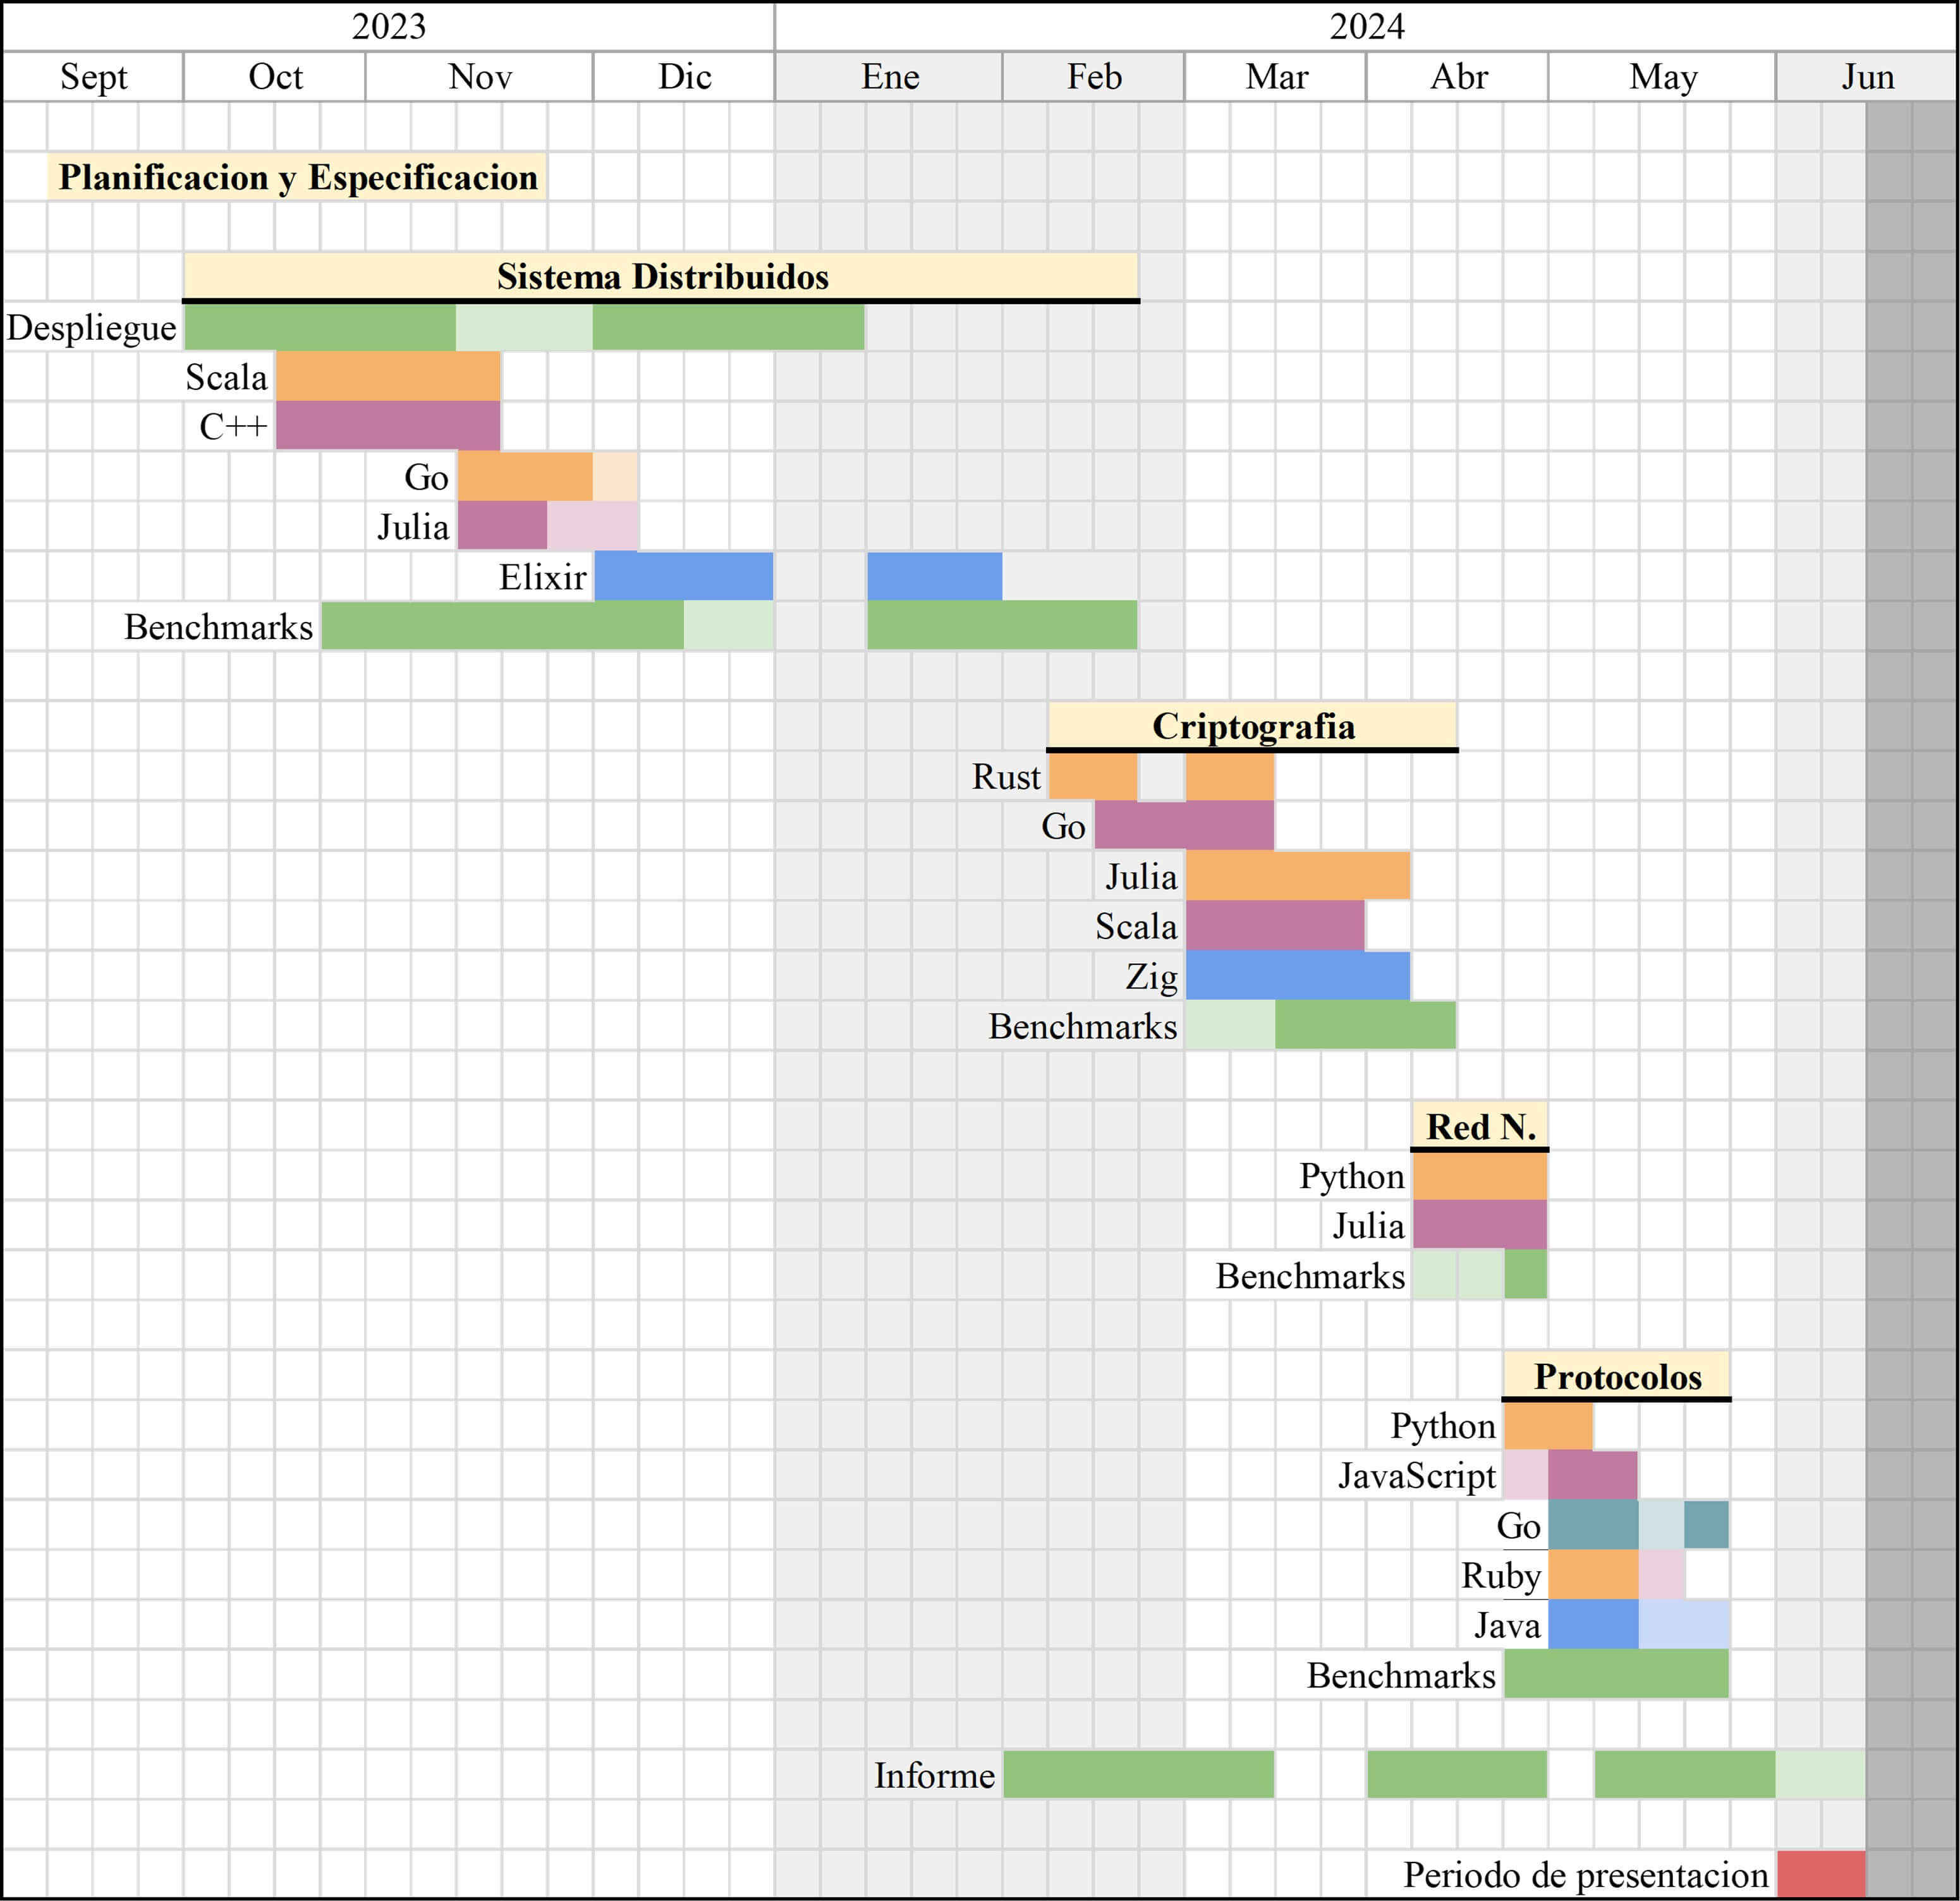
\includegraphics[width=\textwidth]{resources/cronograma.jpg}
    \caption{Cronograma de ejecución de tareas}
    \label{tab:anex:cron}
\end{figure}

Durante la etapa inicial se define el alcance del proyecto, los casos de uso, los lenguajes, las métricas y las especificaciones generales de los desarrollos.

Para cada caso de uso, se pueden observar bloques correspondientes a los lenguajes, que se colorean de manera distinta según el integrante o grupo de integrantes que realizó ese desarrollo.

Además, se identifican ciertas tareas en verde que son complementarias a los desarrollos y pueden requerir la colaboración de todos los integrantes:
\begin{itemize}
    \item \textbf{Despliegue}: Incluye la configuración de los entornos de despliegue y de los sistemas utilizados para la medición de métricas de los contenedores.
    \item \textbf{\english{Benchmarks}}: Incluye la ejecución de los desarrollos y la compilación de métricas.
    \item \textbf{Informe}: Incluye la redacción y edición de este informe.
\end{itemize}

Asimismo, se resaltan algunos periodos de tiempo coloreados de manera más tenue, los cuales indican momentos en los que se planificó desarrollar la tarea indicada, pero no se llevó a cabo el desarrollo.

\subsection{Profiling y optimización de Grid Search en Elixir} \label{sec:anex:elixir_gs_optimization}


Elixir, al ser un lenguaje de programación funcional, representó un desafío adicional para nosotros debido a nuestra falta de familiaridad con este tipo de lenguajes. Una vez finalizado el desarrollo, al ejecutar las métricas del algoritmo de \english{grid search}, la \english{performance} fue decepcionante.

Una métrica que usamos constantemente para comparar la rapidez de procesamiento de los lenguajes fue la de las \english{requests} por segundo (req/s). Esta métrica es adecuada en el caso de \english{grid search}, ya que todos los lenguajes procesan el mismo tamaño de trabajo, por lo que un mayor número de req/s indica un procesamiento más rápido.

En Elixir, en nuestra primera ejecución con dos nodos trabajadores, obtuvimos 0.1 req/s. En comparación, el resto de los lenguajes presentaron desempeños significativamente mejores que este. Estos resultados tan pobres, combinados con nuestra limitada experiencia con el lenguaje, nos llevaron a buscar oportunidades de optimización.

Después de mucha búsqueda e intentos, encontramos una herramienta que resultó de gran ayuda llamada \textit{mix profile}. \textit{Mix profile} es una herramienta integrada en \textit{mix}\footnote{Mix: herramienta propia de Elixir que permite mediante linea de comandos, crear, compilar, ejecutar pruebas y gestionar dependencias de una aplicación.} que genera perfiles de llamadas a funciones a partir de la ejecución de cualquier aplicación de Elixir. Es importante mencionar que esta herramienta es posible gracias a Erlang, ya que Elixir la utiliza a través de su máquina virtual.

\begin{figure}[ht]
    \centering
    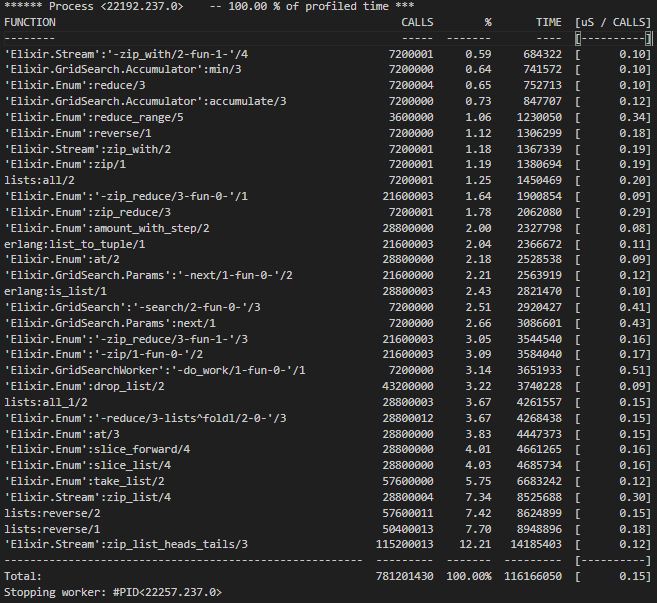
\includegraphics[scale=0.4]{resources/distributed_systems/elixir/1.png}
    \caption{\english{Profiling} en Elixir, primera iteración}
    \label{fig:elx:profiling_1}
\end{figure}

En la Figura~\ref{fig:elx:profiling_1} se muestra el primer \english{profile} que realizamos de nuestro programa. Este perfil corresponde a uno de los nodos trabajadores, ya que representaban el cuello de botella en estas pruebas. Para simplificar el análisis, solo se muestran las funciones que consumen más tiempo de procesamiento. Se puede apreciar el elevado nivel de detalle de este análisis, que nos proporciona no solo la cantidad de llamadas, sino también el tiempo total de procesamiento que requirió cada función, el porcentaje de tiempo en relación a todo el programa y el tiempo por llamada. En esta primera iteración, nos enfocamos en el costo que se incurría al invertir las listas. Gracias a esto, descubrimos que nuestro algoritmo estaba invirtiendo ciertas listas una vez más de lo necesario, por lo que procedimos a hacer los cambios pertinentes, aumentando el \english{throughput} a 0.12 req/s, lo cual representa una mejora del 20\%.

Después de estas mejoras, se generó un nuevo perfil del programa para identificar posibles nuevas optimizaciones. Este segundo perfil se puede ver en la Figura~\ref{fig:elx:profiling_2}.

\begin{figure}[ht]
    \centering
    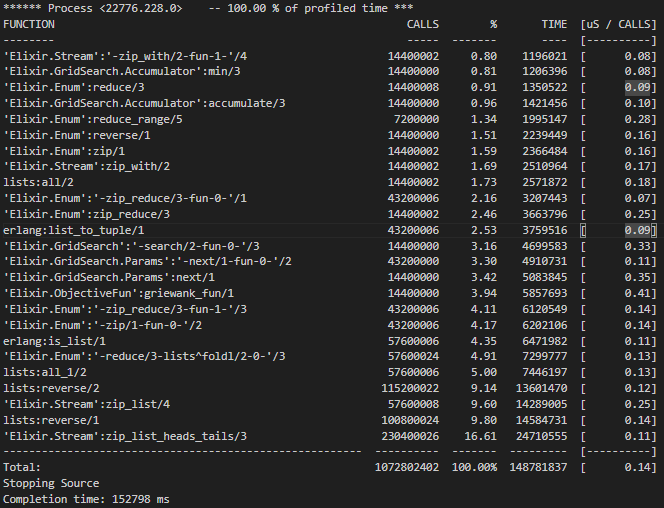
\includegraphics[scale=0.4]{resources/distributed_systems/elixir/2.png}
    \caption{\english{Profiling} en Elixir, segunda iteración}
    \label{fig:elx:profiling_2}
\end{figure}

En esta iteración nos concentramos en las funciones \lstinline{zip} y \lstinline{unzip}, que generaban un considerable gasto de procesamiento. En nuestro algoritmo original, teníamos varias listas de parámetros que se utilizaban para calcular cada grilla del \textit{grid search}. En el código, todos estos parámetros se pasaban a la función \lstinline{reduce}, la cual generaba en cada iteración la entrada para la función de grilla. Para evitar el uso de las funciones \lstinline{zip} y \lstinline{unzip}, se diseñó una nueva estructura de datos que incluyera todos los parámetros.

Con esta mejora, la velocidad de los nodos trabajadores aumentó a 0.2 req/s, lo que representa una mejora del 100\% respecto a nuestra primera versión. En la Figura~\ref{fig:elx:profiling_3} se muestra el perfil del programa con estos cambios implementados.

\begin{figure}[ht]
    \centering
    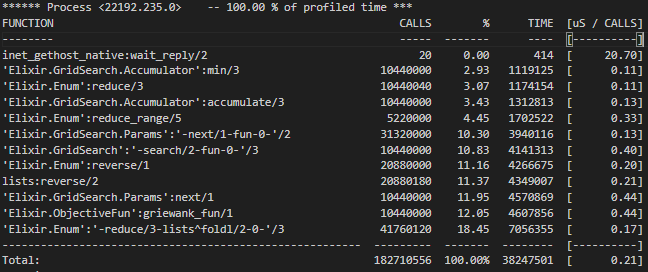
\includegraphics[scale=0.4]{resources/distributed_systems/elixir/3.png}
    \caption{\english{Profiling} en Elixir, iteración final}
    \label{fig:elx:profiling_3}
\end{figure}


Un aspecto relevante que se observa en este perfil es que la función Griewank es la segunda que más tiempo de procesamiento consume del nodo trabajador. Griewank es la función que elegimos para evaluar y optimizar con la búsqueda en grilla. Esto indica que el nodo está dedicando la mayor parte de su tiempo de procesamiento a calcular esta función, lo que sugiere que el programa está cerca del límite teórico de velocidad que puede alcanzar con Elixir.

En conclusión, esta herramienta es sumamente útil, ya que logramos mejoras de hasta un 100\% en la velocidad de nuestro código. Además, la herramienta es muy completa y solo hicimos uso de algunas de sus vastas características. Por ejemplo, esta herramienta es capaz de crear perfiles en aplicaciones concurrentes y distribuidas, utilizando OTP\footnote{OTP: \english{Open Telecom Platform} es un conjunto de bibliotecas proveninentes de BEAM, las cuales permiten la comunicación entre procesos.}, lo que facilita la configuración y el análisis de un sistema complejo en conjunto.

A pesar de la utilidad de la herramienta de \english{profiling}, la búsqueda de esta optimización reveló varios inconvenientes del lenguaje de programación Elixir. El primero es su bajo rendimiento ya que, incluso luego de invertir una buena cantidad de tiempo en optimizaciones, sigue siendo muy inferior al del resto de lenguajes. El segundo es que, a pesar de la simple sintaxis de Elixir, los cambios que se tuvieron que implementar para optimizarlo resultaron en un código desprolijo, difícil de leer y de mantener, lo cual contradice el propósito de este lenguaje.


\subsection{Métricas Extendidas} \label{sec:anex:metrics} 
% FIXME: check that the values of the tables are ok
% FIXME: make descriptions standalone [?] (add section title to desc)

\subsubsection{Grid Search} \label{sec:anex:metrics:gs}

\begin{table}[H]
\centering
\begin{tabular}{|l|c|c|c|}
\hline
\multicolumn{1}{|c|}{Métrica} & 4 Nodos & 8 Nodos & 16 Nodos \\ \hline
\row{\english{Throughput} de los worker\\{[Resultados/Segundo]}} & $2.42$  & $2.28$ & $2.26$ \\ \hline
\row{\english{Throughput} combinado\\{[Resultados/Segundo]}}  & $9.60$  & $18.2$ & $34.8$ \\ \hline
\row{Variación del tiempo\\de trabajo {[\%]}} & $0.83$& $0.25$& $0.38$\\ \hline
\row{Uso de memoria\\{[MB/Trabajador]}} & $1.7-9.0$  & $1.6-9.0$ & $1.3-8.6$ \\ \hline
\row{Uso de red (Tx)\\{[B/(s * Trabajador)]}} & 740 & 710 & 680 \\ \hline
\row{Uso de red (Rx)\\{[B/(s * Trabajador)]}} & 160 & 155 & 150 \\ \hline
\row{Uso de CPU\\{[\%/Trabajador]}} & 100 & 100 & 100 \\ \hline
Tiempo de ejecución [Minutos] & $41.5$ & $22.0$ & $11.2$ \\ \hline
\end{tabular}
\gscap{C++}{FaMAF-2}
\end{table}

\begin{table}[H]
\centering
\begin{tabular}{|l|c|c|c|}
\hline
\multicolumn{1}{|c|}{Métrica} & 4 Nodos & 8 Nodos & 16 Nodos \\ \hline
\row{\english{Throughput} de los worker\\{[Resultados/Segundo]}} & $1.87$ & $1.65$ & $1.68$ \\ \hline
\row{\english{Throughput} combinado\\{[Resultados/Segundo]}} & $7.48$ & $13.2$ & $26.8$ \\ \hline
\row{Variación del tiempo\\de trabajo {[\%]}} & $0.432$ & $0.705$ & $3.80$ \\ \hline
\row{Uso de memoria\\{[MB/Trabajador]}} & $1.29-4.00$ & $1.35-2.95$ & $1.00-4.50$ \\ \hline
\row{Uso de red (Tx)\\{[B/(s * Trabajador)]}} & 580 & 550 & 600 \\ \hline
\row{Uso de red (Rx)\\{[B/(s * Trabajador)]}} & 130 & 130 & 132 \\ \hline
\row{Uso de CPU\\{[\%/Trabajador]}} & 100 & 100 & 100 \\ \hline
Tiempo de ejecución [Minutos] & $54.0$ & $26.7$ & $15.1$ \\ \hline
\end{tabular}
\gscap{C++}{GCP}
\end{table}



\begin{table}[H]
\centering
\begin{tabular}{|l|c|c|c|}
\hline
\multicolumn{1}{|c|}{Métrica} & 4 Nodos & 8 Nodos & 16 Nodos \\ \hline
\row{\english{Throughput} de los worker\\{[Resultados/Segundo]}} & $0.64$ & $0.63$ & $0.6$ \\ \hline
\row{\english{Throughput} combinado\\{[Resultados/Segundo]}} & $2.57$ & $4.85$ & $9.47$ \\ \hline
\row{Variación del tiempo\\de trabajo {[\%]}} & $1.57$ & $1.95$ & $1.83$ \\ \hline
\row{Uso de memoria\\{[MB/Trabajador]}} & 370 & 367 & 360 \\ \hline
\row{Uso de red (Tx)\\{[B/(s * Trabajador)]}} & 352 & 332 & 322 \\ \hline
\row{Uso de red (Rx)\\{[B/(s * Trabajador)]}} & 195 & 184 & 179 \\ \hline
\row{Uso de CPU\\{[\%/Trabajador]}} & 100 & 100 & 100 \\ \hline
Tiempo de ejecución [Minutos] & 155 & 82.2 & $42.1$ \\ \hline
\end{tabular}
\gscap{Scala}{FaMAF-2}
\end{table}



\begin{table}[H]
\centering
\begin{tabular}{|l|c|c|c|}
\hline
\multicolumn{1}{|c|}{Métrica} & 4 Nodos & 8 Nodos & 16 Nodos \\ \hline
\row{\english{Throughput} de los worker\\{[Resultados/Segundo]}} & $0.51$ & $0.51$ & $0.52$ \\ \hline
\row{\english{Throughput} combinado\\{[Resultados/Segundo]}} & $2.03$ & $4.12$ & $8.40$ \\ \hline
\row{Variación del tiempo\\de trabajo {[\%]}} & $3.16$ & $5.04$ & $6.19$ \\ \hline
\row{Uso de memoria\\{[MB/Trabajador]}} & 52-64 & 52-60 & 52-58 \\ \hline
\row{Uso de red (Tx)\\{[B/(s * Trabajador)]}} & 276 & 281 & 285 \\ \hline
\row{Uso de red (Rx)\\{[B/(s * Trabajador)]}} & 153 & 156 & 159 \\ \hline
\row{Uso de CPU\\{[\%/Trabajador]}} & 100 & 100 & 100 \\ \hline
Tiempo de ejecución [Minutos] & $196.8$ & $97.2$ & $47.7$ \\ \hline
\end{tabular}
\gscap{Scala}{GCP}
\end{table}



\begin{table}[H]
\centering
\begin{tabular}{|l|c|c|c|}
\hline
\multicolumn{1}{|c|}{Métrica} & 4 Nodos & 8 Nodos & 16 Nodos \\ \hline
\row{\english{Throughput} de los worker\\{[Resultados/Segundo]}} & $2.07$ & $1.81$ & $1.88$ \\ \hline
\row{\english{Throughput} combinado\\{[Resultados/Segundo]}} & $8.25$ & $14.5$ & $30.2$ \\ \hline
\row{Variación del tiempo\\de trabajo {[\%]}} & $0.686$ & $0.466$ & $0.840$ \\ \hline
\row{Uso de memoria\\{[MB/Trabajador]}} & $6.8-8.4$ & $4.1-8.7$ & $4.0-6.2$ \\ \hline
\row{Uso de red (Tx)\\{[B/(s * Trabajador)]}} & 637 & 598 & 578 \\ \hline
\row{Uso de red (Rx)\\{[B/(s * Trabajador)]}} & 150 & 130 & 126 \\ \hline
\row{Uso de CPU\\{[\%/Trabajador]}} & 100 & 100 & 100 \\ \hline
Tiempo de ejecución [Minutos] & $49.9$ & $27.0$ & $13.4$ \\ \hline
\end{tabular}
\gscap{Go}{FaMAF-2}
\end{table}



\begin{table}[H]
\centering
\begin{tabular}{|l|c|c|c|}
\hline
\multicolumn{1}{|c|}{Métrica} & 4 Nodos & 8 Nodos & 16 Nodos \\ \hline
\row{\english{Throughput} de los worker\\{[Resultados/Segundo]}} & $1.52$ & $1.54$ & $1.51$ \\ \hline
\row{\english{Throughput} combinado\\{[Resultados/Segundo]}} & $5.91$ & $11.7$ & $23.5$ \\ \hline
\row{Variación del tiempo\\de trabajo {[\%]}} & $0.275$ & $5.21$ & $0.644$ \\ \hline
\row{Uso de memoria\\{[MB/Trabajador]}} & $2.4-4.8$ & $1.8-4.4$ & $1.4-2.8$ \\ \hline
\row{Uso de red (Tx)\\{[B/(s * Trabajador)]}} & 462 & 490 & 480 \\ \hline
\row{Uso de red (Rx)\\{[B/(s * Trabajador)]}} & 102 & 104 & 100 \\ \hline
\row{Uso de CPU\\{[\%/Trabajador]}} & 100 & 100 & 100 \\ \hline
Tiempo de ejecución [Minutos] & $67.2$ & $34.2$ & $17.2$ \\ \hline
\end{tabular}
\gscap{Go}{GCP}
\end{table}



\begin{table}[H]
\centering
\begin{tabular}{|l|c|c|c|}
\hline
\multicolumn{1}{|c|}{Métrica} & 4 Nodos & 8 Nodos & 16 Nodos \\ \hline
\row{\english{Throughput} de los worker\\{[Resultados/Segundo]}} & $1.36$ & $1.26$ & $1.26$ \\ \hline
\row{\english{Throughput} combinado\\{[Resultados/Segundo]}} & $5.43$ & $10.1$ & $20.0$ \\ \hline
\row{Variación del tiempo\\de trabajo {[\%]}} & $1.83$ & $1.21$ & $0.757$ \\ \hline
Uso de memoria [GB/Trabajador] & $1.24$ & $1.24$ & $1.18$ \\ \hline
\row{Uso de red (Tx)\\{[B/(s * Trabajador)]}} & 327 & 305 & 302 \\ \hline
\row{Uso de red (Rx)\\{[B/(s * Trabajador)]}} & 220 & 207 & 206 \\ \hline
\row{Uso de CPU\\{[\%/Trabajador]}} & 100 & 100 & 100 \\ \hline
Tiempo de ejecución [Minutos] & $73.2$ & $39.2$ & $20.0$ \\ \hline
\end{tabular}
\gscap{Julia}{FaMAF-2}\label{tab:jl:gs:famaf2}
\end{table}



\begin{table}[H]
\centering
\begin{tabular}{|l|c|c|c|}
\hline
\multicolumn{1}{|c|}{Métrica} & 4 Nodos & 8 Nodos & 16 Nodos \\ \hline
\row{\english{Throughput} de los worker\\{[Resultados/Segundo]}} & $1.18$ & $1.16$ & $1.18$ \\ \hline
\row{\english{Throughput} combinado\\{[Resultados/Segundo]}} & $4.69$ & $9.19$ & $18.8$ \\ \hline
\row{Variación del tiempo\\de trabajo {[\%]}} & $2.40$ & $1.58$ & $2.19$ \\ \hline
Uso de memoria [GB/Trabajador] & $1.10$ & $1.08$ & $1.09$ \\ \hline
\row{Uso de red (Tx)\\{[B/(s * Trabajador)]}} & 280 & 276 & 282 \\ \hline
\row{Uso de red (Rx)\\{[B/(s * Trabajador)]}} & 189 & 187 & 194 \\ \hline
\row{Uso de CPU\\{[\%/Trabajador]}} & 100 & 100 & 100 \\ \hline
Tiempo de ejecución [Minutos] & $85.2$ & $43.3$ & $21.3$ \\ \hline
\end{tabular}
\gscap{Julia}{GCP}
\end{table}



\begin{table}[H]
\centering
\begin{tabular}{|l|c|c|c|}
\hline
\multicolumn{1}{|c|}{Métrica} & 4 Nodos & 8 Nodos & 16 Nodos \\ \hline
\row{\english{Throughput} de los worker\\{[Resultados/Segundo]}} & $0.25$ & $0.24$ & $0.23$ \\ \hline
\row{\english{Throughput} combinado\\{[Resultados/Segundo]}} & $0.991$ & $1.90$ & $3.74$ \\ \hline
\row{Variación del tiempo\\de trabajo {[\%]}} & $3.05$ & 659 & $2.37$ \\ \hline
\row{Uso de memoria\\{[MB/Trabajador]}} & 83-95 & 84-96 & 84 \\ \hline
\row{Uso de red (Tx)\\{[B/(s * Trabajador)]}} & 376 & 399 & 469 \\ \hline
\row{Uso de red (Rx)\\{[B/(s * Trabajador)]}} & 266 & 296 & 367 \\ \hline
\row{Uso de CPU\\{[\%/Trabajador]}} & 100 & 100 & 100 \\ \hline
Tiempo de ejecución [Minutos] & $403.2$ & $209.4$ & $106.8$ \\ \hline
\end{tabular}
\gscap{Elixir}{FaMAF-2}
\end{table}



\begin{table}[H]
\centering
\begin{tabular}{|l|c|c|c|c|c|}
\hline
\multicolumn{1}{|c|}{Métrica} & C++ & Scala & Go & Julia & Elixir \\ \hline
\row{\english{Throughput} combinado \\ {[Resultados/Segundo]}} & $18.2$ & $4.85$ & $14.5$ & $10.1$ & $1.90$ \\ \hline
\row{Variación del tiempo \\ de trabajo {[}\%{]}} & $0.25$ & $1.95$ & $0.466$ & $1.21$ & $0.659$ \\ \hline
\row{Uso de memoria \\ {[}MB/Trabajador{]}} & $1.6-9.0$ & 367 & $4.1-8.7$ & \numprint{1240} & 84-96 \\ \hline
\row{Uso de red (Tx)\\ {[}B/(s * Trabajador){]}} & 710 & 332 & 598 & 305 & 399 \\ \hline
\row{Uso de red (Rx)\\ {[}B/(s * Trabajador){]}} & 155 & 184 & 130 & 207 & 296 \\ \hline
Tiempo de ejecución {[}Minutos{]} & $22.0$ & $82.2$ & $27.0$ & $39.2$ & $209.4$ \\ \hline
\end{tabular}
\caption{Resumen de métricas corridas con 8 Workers en FaMAF-2, para el caso de uso de Grid Search}
\label{tab:gs:8_workers_famaf2}
\end{table}


\begin{table}[H]
\centering
\begin{tabular}{|l|c|c|c|c|c|}
\hline
\multicolumn{1}{|c|}{Métrica} & C++ & Scala & Go & Julia & Elixir \\ \hline
\row{\english{Throughput} combinado\\{[Resultados/Segundo]}} & $13.2$ & $4.12$ & $11.7$ & $9.19$ & - \\ \hline
\row{Variación del tiempo \\ de trabajo {[}\%{]}} & $0.705$ & $5.04$ & $5.21$ & $1.58$ & - \\ \hline
\row{Uso de memoria \\ {[}MB/Trabajador{]}} & $1.35-2.95$ & 52-60 & $1.8-4.4$ & \numprint{1080} & - \\ \hline
\row{Uso de red (Tx)\\ {[}B/(s * Trabajador){]}} & 550 & 281 & 490 & 276 & - \\ \hline
\row{Uso de red (Rx)\\ {[}B/(s * Trabajador){]}} & 130 & 156 & 104 & 187 & - \\ \hline
Tiempo de ejecución {[}Minutos{]} & $26.7$ & $97.2$ & $34.2$ & $43.3$ & - \\ \hline
\end{tabular}
\caption{Resumen de métricas corridas con 8 Workers en GCP, para el caso de uso de Grid Search}
\label{tab:gs:image_sizes}
\end{table}


\begin{table}[H]
\centering
\begin{tabular}{|ccc|}
\hline
\multicolumn{1}{|c|}{\multirow{2}{*}{C++}} & \multicolumn{1}{c|}{Manager} & $17.4$ MB \\ \cline{2-3} 
\multicolumn{1}{|c|}{} & \multicolumn{1}{c|}{Worker} & $17.3$ MB \\ \hline
\multicolumn{1}{|c|}{\multirow{3}{*}{Scala}} & \multicolumn{1}{c|}{Manager} & 192 MB \\ \cline{2-3} 
\multicolumn{1}{|c|}{} & \multicolumn{1}{c|}{Worker} & 192 MB \\ \cline{2-3} 
\multicolumn{1}{|c|}{} & \multicolumn{1}{c|}{Middleware} & 180 MB \\ \hline
\multicolumn{1}{|c|}{\multirow{3}{*}{Go}} & \multicolumn{1}{c|}{Manager} & $15.5$ MB \\ \cline{2-3} 
\multicolumn{1}{|c|}{} & \multicolumn{1}{c|}{Worker} & $15.4$ MB \\ \cline{2-3} 
\multicolumn{1}{|c|}{} & \multicolumn{1}{c|}{Middleware} & $14.4$ MB \\ \hline
\multicolumn{1}{|c|}{\multirow{2}{*}{Julia}} & \multicolumn{1}{c|}{Manager} & 754 MB \\ \cline{2-3} 
\multicolumn{1}{|c|}{} & \multicolumn{1}{c|}{Worker} & 795 MB \\ \hline
\multicolumn{1}{|c|}{\multirow{2}{*}{Elixir}} & \multicolumn{1}{c|}{Manager} & \textgreater{}84.8MB \\ \cline{2-3} 
\multicolumn{1}{|c|}{} & \multicolumn{1}{c|}{Worker} & \textgreater{}84.8MB \\ \hline
\end{tabular}
\caption{Tamaño de imágenes de Docker para el caso de uso de Grid Search}
\end{table}

\subsubsection{Procesamiento de Imágenes} \label{sec:anex:metrics:ip}

\begin{table}[H]
\centering
\begin{tabular}{|l|c|c|c|}
\hline
\multicolumn{1}{|c|}{Métrica} & 2 Nodos & 4 Nodos & 6 Nodos \\ \hline
\row{\english{Throughput} combinado\\{[Resultados/Segundo]}} & 172 & 250 & 263 \\ \hline
\row{Máxima variacaión del \\ tiempo de trabajo {[}\%{]}} & $5.5$ & $2.8$ & $5.6$ \\ \hline
\row{Máximo uso de memoria \\ {[MB/Trabajador]}} & 70 & 55 & 41 \\ \hline
\row{Máximo uso de red (Tx) \\ {[KB/(s * Trabajador)]}} & 32 & 22 & 14 \\ \hline
\row{Máximo uso de red (Tx) \\ {[KB/(s * Trabajador)]}} & 18 & 12 & $1.2$  \\ \hline
\row{Uso de CPU - Formato\\{[\%/Trabajador]}} & 100 & 75  & 50 \\ \hline
\row{Uso de CPU - Resolución\\{[\%/Trabajador]}} & 56 & 40 & 35 \\ \hline
\row{Uso de CPU - Tamaño\\{[\%/Trabajador]}} & 18 & 10 & 10 \\ \hline
Tiempo de ejecución [Minutos] & $26.1$ & $18.0$ & $17.1$ \\ \hline
\end{tabular}
\ipcap{C++}{FaMAF-2}
\end{table}


\begin{table}[H]
\centering
\begin{tabular}{|l|c|c|c|}
\hline
\multicolumn{1}{|c|}{Métrica} & 2 Nodos & 4 Nodos & 6 Nodos \\ \hline
\row{\english{Throughput} combinado\\{[Resultados/Segundo]}} & $75.2$ & $84$ & $119$ \\ \hline
\row{Máxima variacaión del \\ tiempo de trabajo {[}\%{]}} & $1.1$ & $1.9$ & $3.3$ \\ \hline
\row{Máximo uso de memoria \\ {[MB/Trabajador]}} & 180 & 97 & 75 \\ \hline
\row{Máximo uso de red (Tx) \\ {[KB/(s * Trabajador)]}} & 13 & $6.9$ & $6.8$ \\ \hline
\row{Máximo uso de red (Tx) \\ {[KB/(s * Trabajador)]}} & $7.2$ & $3.8$ & $3.8$ \\ \hline
\row{Uso de CPU - Formato\\{[\%/Trabajador]}} & 60 & 35 & 35 \\ \hline
\row{Uso de CPU - Resolución\\{[\%/Trabajador]}} & 22 & 10 & 12 \\ \hline
\row{Uso de CPU - Tamaño\\{[\%/Trabajador]}} & 7 & 5 & 5 \\ \hline
Tiempo de ejecución [Minutos] & $19.9$ & $17.8$ & $12.6$ \\ \hline
\end{tabular}
\ipcap{C++}{GCP}
\end{table}


\begin{table}[H]
\centering
\begin{tabular}{|l|c|c|c|}
\hline
\multicolumn{1}{|c|}{Métrica} & 2 Nodos & 4 Nodos & 6 Nodos \\ \hline
\row{\english{Throughput} combinado\\{[Resultados/Segundo]}} & 117 & 139 & 162 \\ \hline
\row{Máxima variacaión del \\ tiempo de trabajo {[}\%{]}} & $0.8$ & $3.2$ & $2.7$ \\ \hline
\row{Máximo uso de memoria \\ {[MB/Trabajador]}} & 830 & 715 & 660 \\ \hline
\row{Máximo uso de red (Tx) \\ {[KB/(s * Trabajador)]}} & 24 & 15 & 12 \\ \hline
\row{Máximo uso de red (Tx) \\ {[KB/(s * Trabajador)]}} & 18 & 11 & $8.9$ \\ \hline
\row{Uso de CPU - Formato\\{[\%/Trabajador]}} & 85 & 55 & 41 \\ \hline
\row{Uso de CPU - Resolución\\{[\%/Trabajador]}} & 65 & 38 & 30 \\ \hline
\row{Uso de CPU - Tamaño\\{[\%/Trabajador]}} & 19 & 10 & 8 \\ \hline
Tiempo de ejecución [Minutos] & $38.4$ & $32.3$ & $27.7$ \\ \hline
\end{tabular}
\ipcap{Scala}{FaMAF-2}
\end{table}


\begin{table}[H]
\centering
\begin{tabular}{|l|c|c|c|}
\hline
\multicolumn{1}{|c|}{Métrica} & 2 Nodos & 4 Nodos & 6 Nodos \\ \hline
\row{\english{Throughput} combinado\\{[Resultados/Segundo]}} & $75.3$ & 109 & 153 \\ \hline
\row{Máxima variacaión del \\ tiempo de trabajo {[}\%{]}} & $4.3$ & $2.4$ & $8.6$ \\ \hline
\row{Máximo uso de memoria \\ {[MB/Trabajador]}} & 330 & 240 & 200 \\ \hline
\row{Máximo uso de red (Tx) \\ {[KB/(s * Trabajador)]}} & 15 & 12 & 11 \\ \hline
\row{Máximo uso de red (Tx) \\ {[KB/(s * Trabajador)]}} & 11 & $1.4$ & $1.0$ \\ \hline
\row{Uso de CPU - Formato\\{[\%/Trabajador]}} & 64 & 44 & 42 \\ \hline
\row{Uso de CPU - Resolución\\{[\%/Trabajador]}} & 37 & 28 & 27 \\ \hline
\row{Uso de CPU - Tamaño\\{[\%/Trabajador]}} & 13 & 8 & 9 \\ \hline
Tiempo de ejecución [Minutos] & $19.9$ & $13.7$ & $9.8$ \\ \hline
\end{tabular}
\ipcap{Scala}{GCP}
\end{table}


\begin{table}[H]
\centering
\begin{tabular}{|l|c|c|c|}
\hline
\multicolumn{1}{|c|}{Métrica} & 2 Nodos & 4 Nodos & 6 Nodos \\ \hline
\row{\english{Throughput} combinado\\{[Resultados/Segundo]}} & 50 & 92 & 135 \\ \hline
\row{Máxima variacaión del \\ tiempo de trabajo {[}\%{]}} & $2.11$ & $5.78$ & $9.42$ \\ \hline
\row{Máximo uso de memoria \\ {[MB/Trabajador]}} & 128 & 96 & 68 \\ \hline
\row{Máximo uso de red (Tx) \\ {[KB/(s * Trabajador)]}} & $7.85$ & $7.21$ & $7.03$ \\ \hline
\row{Máximo uso de red (Tx) \\ {[KB/(s * Trabajador)]}} & $5.51$ & $4.23$ & $4.16$ \\ \hline
\row{Uso de CPU - Formato\\{[\%/Trabajador]}} & 100 & 100 & 100 \\ \hline
\row{Uso de CPU - Resolución\\{[\%/Trabajador]}} & 80 & 80 & 80 \\ \hline
\row{Uso de CPU - Tamaño\\{[\%/Trabajador]}} & 20 & 20 & 20 \\ \hline
Tiempo de ejecución [Minutos] & $89.9$ & $48.8$ & $33.3$ \\ \hline
\end{tabular}
\ipcap{Go}{FaMAF-2}
\end{table}


\begin{table}[H]
\centering
\begin{tabular}{|l|c|c|c|}
\hline
\multicolumn{1}{|c|}{Métrica} & 2 Nodos & 4 Nodos & 6 Nodos \\ \hline
\row{\english{Throughput} combinado\\{[Resultados/Segundo]}} & 40 & 75 & 104 \\ \hline
\row{Máxima variacaión del \\ tiempo de trabajo {[}\%{]}} & $2.96$ & $11.3$ & $24.9$ \\ \hline
\row{Máximo uso de memoria \\ {[MB/Trabajador]}} & 144 & 90 & 64 \\ \hline
\row{Máximo uso de red (Tx) \\ {[KB/(s * Trabajador)]}} & $6.03$ & $5.62$ & $5.20$ \\ \hline
\row{Máximo uso de red (Rx) \\ {[KB/(s * Trabajador)]}} & $3.58$ & $3.37$ & $3.12$ \\ \hline
\row{Uso de CPU - Formato\\{[\%/Trabajador]}} & 80 & 80 & 80 \\ \hline
\row{Uso de CPU - Resolución\\{[\%/Trabajador]}} & 30 & 30 & 25 \\ \hline
\row{Uso de CPU - Tamaño\\{[\%/Trabajador]}} & 5 & 5 & 5 \\ \hline
Tiempo de ejecución [Minutos] & $37.5$ & $20.0$ & $14.4$ \\ \hline
\end{tabular}
\ipcap{Go}{GCP}
\end{table}


\begin{table}[H]
\centering
\begin{tabular}{|l|c|c|c|}
\hline
\multicolumn{1}{|c|}{Métrica} & 2 Nodos & 4 Nodos & 6 Nodos \\ \hline
\row{\english{Throughput} combinado\\{[Resultados/Segundo]}} & 400 & 745 & \numprint{1100} \\ \hline
\row{Máxima variacaión del \\ tiempo de trabajo {[}\%{]}} & $1.7$ & $1.5$ & 8 \\ \hline
\row{Máximo uso de memoria \\ {[MB/Trabajador]}} & 448 & 460 & 450 \\ \hline
\row{Máximo uso de red (Tx) \\ {[KB/(s * Trabajador)]}} & 136 & 125 & 118 \\ \hline
\row{Máximo uso de red (Rx) \\ {[KB/(s * Trabajador)]}} & 55 & 50 & 48 \\ \hline
\row{Uso de CPU - Formato\\{[\%/Trabajador]}} & 92 & 96 & 96 \\ \hline
\row{Uso de CPU - Resolución\\{[\%/Trabajador]}} & 73 & 69 & 72 \\ \hline
\row{Uso de CPU - Tamaño\\{[\%/Trabajador]}} & 34 & 31 & 30 \\ \hline
Tiempo de ejecución [Minutos] & $11.2$ & $6.0$ & $4.1$ \\ \hline
\end{tabular}
\ipcap{Julia}{FaMAF-2}
\end{table}


\begin{table}[H]
\centering
\begin{tabular}{|l|c|c|c|}
\hline
\multicolumn{1}{|c|}{Métrica} & 2 Nodos & 4 Nodos & 6 Nodos \\ \hline
\row{\english{Throughput} combinado\\{[Resultados/Segundo]}} & 82.6 & 215 & 235 \\ \hline
\row{Máxima variacaión del \\ tiempo de trabajo {[}\%{]}} & $6.5$ & $5.7$ & $8.3$ \\ \hline
\row{Máximo uso de memoria \\ {[MB/Trabajador]}} & \numprint{1130} & 896 & 704 \\ \hline
\row{Máximo uso de red (Tx) \\ {[KB/(s * Trabajador)]}} & 28 & 37 & 27 \\ \hline
\row{Máximo uso de red (Rx) \\ {[KB/(s * Trabajador)]}} & 11 & 15 & 11 \\ \hline
\row{Uso de CPU - Formato\\{[\%/Trabajador]}} & 24 & 38 & 25 \\ \hline
\row{Uso de CPU - Resolución\\{[\%/Trabajador]}} & 18 & 24 & 19 \\ \hline
\row{Uso de CPU - Tamaño\\{[\%/Trabajador]}} & 9 & 11 & 7 \\ \hline
Tiempo de ejecución [Minutos] & $18.1$ & $6.9$ & $6.37$ \\ \hline
\end{tabular}
\ipcap{Julia}{GCP}
\end{table}

\begin{table}[H]
\centering
\begin{tabular}{|l|c|c|c|}
\hline
\multicolumn{1}{|c|}{Métrica} & 2 Nodos & 4 Nodos & 6 Nodos \\ \hline
\row{\english{Throughput} combinado\\{[Resultados/Segundo]}} & $78.2$ & 141 & 245 \\ \hline
\row{Máxima variación del\\tiempo de trabajo [\%]} & $1.3$ & $2.3$ & $2.0$ \\ \hline
\row{Máximo uso de memoria\\{[MB/Trabajador]}} & 140 & 115 & 650 \\ \hline
\row{Máximo uso de red (Tx)\\{[KB/(s * Trabajador)]}} & $9.2$ & $8.2$ & $9.4$ \\ \hline
\row{Máximo uso de red (Rx)\\{[KB/(s * Trabajador)]}} & $3.4$ & $3.0$ & $3.6$ \\ \hline
\row{Uso de CPU - Formato\\ {[\%/Trabajador]}} & 96 & 77 & 77 \\ \hline
\row{Uso de CPU - Resolución\\ {[\%/Trabajador]}} & 110 & 93 & 92 \\ \hline
\row{Uso de CPU - Tamaño\\ {[\%/Trabajador]}} & 33 & 25 & 26 \\ \hline
Tiempo de ejecución {[Minutos]} & $57.5$ & $31.9$ & $18.3$ \\ \hline
\end{tabular}
\ipcap{Elixir}{FaMAF-2}
\end{table}

\begin{table}[H]
\centering
\begin{tabular}{|l|c|c|c|}
\hline
\multicolumn{1}{|c|}{Métrica} & 2 Nodos & 4 Nodos & 6 Nodos \\ \hline
\row{\english{Throughput} combinado \\ {[Resultados/Segundo]}} & $57.6$ & $85.1$ & 103 \\ \hline
\row{Máxima variación del \\ tiempo de trabajo {[\%]}} & $3.6$ & $5.6$ & $6.6$ \\ \hline
\row{Máximo uso de memoria \\ {[MB/Trabajador]}} & 390 & 240 & 180 \\ \hline
\row{Máximo uso de red (Tx) \\ {[KB/(s * Trabajador)]}} & $6.6$ & $4.8$ & $1.0$ \\ \hline
\row{Máximo uso de red (Rx)\\{[KB/(s * Trabajador)]}} & $2.3$ & $1.8$ & $1.5$ \\ \hline
\row{Uso de CPU - Formato\\{[\%/Trabajador]}} & 44 & 35 & 28 \\ \hline
\row{Uso de CPU - Resolución\\{[\%/Trabajador]}} & 26 & 20 & 18 \\ \hline
\row{Uso de CPU - Tamaño\\{[\%/Trabajador]}} & 18 & 16 & 12 \\ \hline
\row{Tiempo de ejecución [Minutos]} & $26.0$ & $17.6$ & $14.54$ \\ \hline
\end{tabular}
\ipcap{Elixir}{GCP}
\end{table}


\begin{table}[H]
\centering
\begin{tabular}{|l|c|c|c|c|c|}
\hline
\multicolumn{1}{|c|}{Métrica} & C++ & Scala & Go & Julia & Elixir \\ \hline
\row{\english{Throughput} combinado\\ {[}Resultados/Segundo{]}} & 250 & 139 & 92 & 745 & 141 \\ \hline
\row{Máxima variacaión del \\ tiempo de trabajo {[}\%{]}} & $2.8$ & $3.2$ & $5.78$ & $1.5$ & $2.3$ \\ \hline
\row{Uso máximo de memoria \\ {[}MB/Trabajador{]}} & 55 & 715 & 96 & 460 & 115 \\ \hline
\row{Uso máximo de la red (Tx)\\ {[}KB/(s * Trabajador){]}} & 22 & 15 & $7.21$ & 125 & $8.2$ \\ \hline
\row{Uso máximo de la red (Rx)\\ {[}KB/(s * Trabajador){]}} & 12 & 11 & $4.23$ & 50 & $3.0$ \\ \hline
\row{Uso de CPU - Formato \\ {[}\%/Trabajador{]}} & 75 & 55 & 100 & 96 & 77 \\ \hline
\row{Uso de CPU - Resolución \\ {[}\%/Trabajador{]}} & 40 & 38 & 80 & 69 & 93 \\ \hline
\row{Uso de CPU - Tamaño \\ {[}\%/Trabajador{]}} & 10 & 10 & 20 & 31 & 25 \\ \hline
Tiempo de ejecución {[}Minutos{]} & $18.0$ & $32.3$ & $48.8$ & $6.0$ & $17.4$ \\ \hline
\end{tabular}
\caption{Resumen de métricas ejecutadas con 4 nodos por etapa en FaMAF-2, para el caso de uso de Procesamiento de Imágenes}
\label{tab:ip:4_workers_famaf_2}
\end{table}


\begin{table}[H]
\centering
\begin{tabular}{|l|c|c|c|c|c|}
\hline
\multicolumn{1}{|c|}{Métrica} & C++ & Scala & Go & Julia & Elixir \\ \hline
\row{\english{Throughput} combinado \\ {[Resultados/Segundo]}} & 84 & 109 & 75 & 215 & $85.1$ \\ \hline
\row{Máxima variacaión del \\ tiempo de trabajo {[}\%{]}} & $1.9$ & $2.4$ & $11.3$ & $5.7$ & $5.6$ \\ \hline
\row{Uso máximo de memoria \\ {[}MB/Trabajador{]}} & 97 & 240 & 90 & 896 & 240 \\ \hline
\row{Uso máximo de la red (Tx) \\ {[}KB/(s * Trabajador){]}} & $6.9$ & 12 & $5.62$ & 37 & $4.8$ \\ \hline
\row{Uso máximo de la red (Rx)\\ {[}KB/(s * Trabajador){]}} & $3.8$ & $8.4$ & $3.37$ & 15 & $1.8$ \\ \hline
\row{Uso de CPU - Formato \\ {[\%/Trabajador]}} & 35 & 44 & 80 & 38 & 35 \\ \hline
\row{Uso de CPU - Resolución \\ {[\%/Trabajador]}} & 10 & 28 & 30 & 24 & 20 \\ \hline
\row{Uso de CPU - Tamaño \\ {[\%/Trabajador]}} & 5 & 8 & 5 & 11 & 16 \\ \hline
Tiempo de ejecución {[}Minutos{]} & $17.8$ & $13.7$ & $20.0$ & $1.9$ & $17.6$ \\ \hline
\end{tabular}
\caption{Resumen de métricas ejecutadas con 4 nodos por etapa en GCP, para el caso de uso de Procesamiento de Imágenes}
\end{table}


\begin{table}[H]
\centering
\begin{tabular}{|ccc|}
\hline
\multicolumn{1}{|c|}{\multirow{3}{*}{C++}} & \multicolumn{1}{c|}{Manager} & $1.45$ GB \\ \cline{2-3} 
\multicolumn{1}{|c|}{} & \multicolumn{1}{c|}{Worker} & $1.45$ GB \\ \cline{2-3} 
\multicolumn{1}{|c|}{} & \multicolumn{1}{c|}{Middleware} & $1.45$ GB \\ \hline
\multicolumn{1}{|c|}{\multirow{3}{*}{Scala}} & \multicolumn{1}{c|}{Manager} & 194 MB \\ \cline{2-3} 
\multicolumn{1}{|c|}{} & \multicolumn{1}{c|}{Worker} & 194 MB \\ \cline{2-3} 
\multicolumn{1}{|c|}{} & \multicolumn{1}{c|}{Middleware} & 180 MB \\ \hline
\multicolumn{1}{|c|}{\multirow{3}{*}{Go}} & \multicolumn{1}{c|}{Manager} & 15 MB \\ \cline{2-3} 
\multicolumn{1}{|c|}{} & \multicolumn{1}{c|}{Worker} & $15.8$ MB \\ \cline{2-3} 
\multicolumn{1}{|c|}{} & \multicolumn{1}{c|}{Middleware} & $14.4$ MB \\ \hline
\multicolumn{1}{|c|}{\multirow{2}{*}{Julia}} & \multicolumn{1}{c|}{Manager} & $1.96$ GB \\ \cline{2-3} 
\multicolumn{1}{|c|}{} & \multicolumn{1}{c|}{Worker} & $1.96$ GB \\ \hline
\multicolumn{1}{|c|}{\multirow{2}{*}{Elixir}} & \multicolumn{1}{c|}{Manager} & \textgreater{}$84.8$ MB \\ \cline{2-3} 
\multicolumn{1}{|c|}{} & \multicolumn{1}{c|}{Worker} & \textgreater{}$84.8$ MB \\ \hline
\end{tabular}
\caption{Tamaño de imágenes de Docker para el caso de uso de Procesamiento de Imágenes}
\label{tab:ip:image_sizes}
\end{table}

\subsubsection{Criptografía: AES} \label{sec:anex:metrics:aes}

\begin{table}[H]
\centering
\begin{tabular}{|c|c|c|c|c|c|}
\hline
Métrica & Rust & Go & Julia & Scala & Zig \\ \hline
Duración [Minutos] & $16.9$ & 102 & $15.9$ & 252 & $24.3$ \\ \hline
Uso de memoria [MB] & 231 & $15.9$ & 548 & 566 & $2.27$ \\ \hline
Uso de CPU [\%] & 300 & 337 & 229 & 179 & 232 \\ \hline
\end{tabular}
\caption{Resumen de métricas del área de criptografía en FaMAF-2. Un uso del CPU del 100\% significa que el proceso utilizó, en promedio, un único \english{core}}
\label{tab:aes:famaf_2}
\end{table}

\begin{table}[H]
\centering
\begin{tabular}{|c|c|}
\hline
Rust & $4.39$ MB \\ \hline
Go & $11.3$ MB \\ \hline
Julia & 716 MB \\ \hline
Scala & 192 MB \\ \hline
Zig & $11.7$ MB \\ \hline
\end{tabular}
\caption{Tamaño de imágenes de Docker para el caso de uso de Criptografía}
\label{tab:aes:container_metrics}
\end{table}

\subsubsection{Redes neuronales: Regresión} \label{sec:anex:metrics:nn}

\begin{table}[H]
\centering
\begin{tabular}{|c|c|c|c|c|}
\hline
& \multicolumn{2}{c|}{Python} & \multicolumn{2}{c|}{Julia} \\ \hline
Métrica & Tensorflow/Keras & PyTorch & Flux & SciKitLearn \\ \hline
Duración [Minutos] & 21 & $7.3$ & $2.56$ & $0.35$ \\ \hline
Uso de memoria [GB] & $2.55$ & $3.16$ & $2.69$ & $1.33$ \\ \hline
Uso de CPU [\%] & $126.00$ & $99.99$& $106.00$& $105.00$\\ \hline
Uso de GPU [GB] & $6.76$ & $1.08$ & $0.69$ & - \\ \hline
Raíz del error cuadrático medio [USD] & \numprint{50500} & \numprint{52582} & \numprint{53400} & \numprint{49000} \\ \hline
\end{tabular}
\caption{Resumen de métricas del área de redes neuronales, en FaMAF-2. Un uso del CPU del 100\% significa que el proceso utilizó, en promedio, un único \english{core}}
\label{tab:nn:famaf_2}
\end{table}

\subsubsection{Protocolos de comunicación: HTTP}

\begin{table}[H]
\centering
\begin{tabular}{|c|c|c|c|c|c|}
\hline
Métrica       & Go   & Java & Python & Ruby & JavaScript \\ \hline
Uso de CPU [\%]         & $58.3$ & 582  & 1701   & 1398 & 180        \\ \hline
Uso de memoria [MB]   & $55.2$ & 512  & 1620   & 2280 & 112        \\ \hline
Latencia [Milisegundos]   & $100$  & 250  & 400    & 380  & 130        \\ \hline
\english{Throughput} [Escenarios/segundo] & $70$   & 70   & 60     & 60   & 20         \\ \hline
\end{tabular}
\caption{Resumen de métricas del área de protocolos de comunicación, en FaMAF-2. Un uso del CPU del 100\% significa que el proceso utilizó, en promedio, un único \english{core} }
\label{tab:http:famaf_1}
\end{table}

\end{document}
